% build/Report-Body.tex
% Simon Hulse
% simonhulse@protonmail.com
% Last Edited: Wed 27 Nov 2024 03:05:28 PM EST

\documentclass[final,%
               twoside,%
               openany,%
               tightbibliography,%
               dontusefourier,%
               thawtoc,%
               doublespace]{oxchempartii-report}
\raggedbottom

\DeclareSIUnit{\myhertz}{Hz}

\usepackage{afterpage}
\newcommand\blankpage{%
    \null
    \thispagestyle{empty}%
    \addtocounter{page}{-1}%
    \newpage}
\let\epsilon\varepsilon
%%% Data for title page %%%%%%%%%%%%%%%%%%%%%%%%%%%%%%%%%%%%
\title{An Investigation of Relaxation Phenomena in I$_3$S Nuclear Spin Systems}
\subtitle{Analysing the Feasibility of a $^{13}$CF$_3$ TROSY Experiment}
\author{Simon Hulse}
\college{Jesus College}
\typeofdocument{A thesis submitted for the\\ Honour School of Chemistry:\\ Chemistry Part II, 2019}
\date{14 June 2019}% Defaults to \today if left empty.
\institution{Physical and Theoretical Chemistry Laboratory}
%%%%%%%%%%%%%%%%%%%%%%%%%%%%%%%%%%%%%%%%%%%%%%%%%%%%%%%%%%%
\usetikzlibrary{patterns}
\makeatletter
\let\thetitle\@title
\let\thesubtitle\@subtitle
\let\theauthor\@author
\let\thecollege\@college
\let\thedate\@date
\makeatother

\allowdisplaybreaks


\begin{document}
% This line silences errors where both the summary and your real start
% are both numbered from one, and laTeX doesn't know where to hyperlink
\hypersetup{pageanchor=false}
\frontmatter
\makeoxtitle{./Other/OxfordCrest.eps}

\let\cleardoublepage\clearpage
% !TeX root = ./Report-Body.tex
\chapter{Summary}%

% Write the Summary text inside the summarytext environment.

% Put the Summary references in PartII-SummaryReferences.bib

\begin{summarytext}
NMR spectroscopy is a highly valuable technique for the characterisation of structure and dynamics of biomolecules. Despite this, the effects of relaxation limits the size of molecules that can be studied. Transverse Relaxation Optimised Spectroscopy (TROSY) is a method which has increased this limit, though there is a desire to push it even further.\\
We believe that a TROSY experiment which probes $^{13}$CF$_3$ moieties could allow studies of macromolecules which are currently deemed too large, in the context of solution-state NMR. Such systems include membrane-bound proteins and virus particles.\\
A novel relaxation theory is presented that is well-suited to describe $^{13}$CF$_3$ systems. Comparisons of relaxation behaviour between methyl and $^{13}$CF$_3$ groups were made using our theory. Our results indicate that magnetisations associated with $^{13}$CF$_3$ moieties relax at noticeably slower rates. This observation was determined to be driven largely by dipolar coupling effects, with the $^{19}$F chemical shift anisotropy also playing a significant role. These findings show that the development of a $^{13}$CF$_3$ TROSY experiment is a worthwhile pursuit, which could extend the scope of NMR.\\
Validation of this theory was achieved via studies on a small $^{13}$CH$_3$-labelled molecule, present in a highly viscous medium. Although our theory described its relaxation well, the molecule was not effective at mimicking proteins.\\
\end{summarytext}


\AtNextBibliography{\footnotesize}
%\begin{singlespacing}
%\printsummarybibliography
%\end{singlespacing}

\let\cleardoublepage\clearpage
\tableofcontents

\let\cleardoublepage\clearpage
% %%% You do not need to edit this file
%
\addcontentsline{toc}{chapter}{Declaration of Authorship}
%
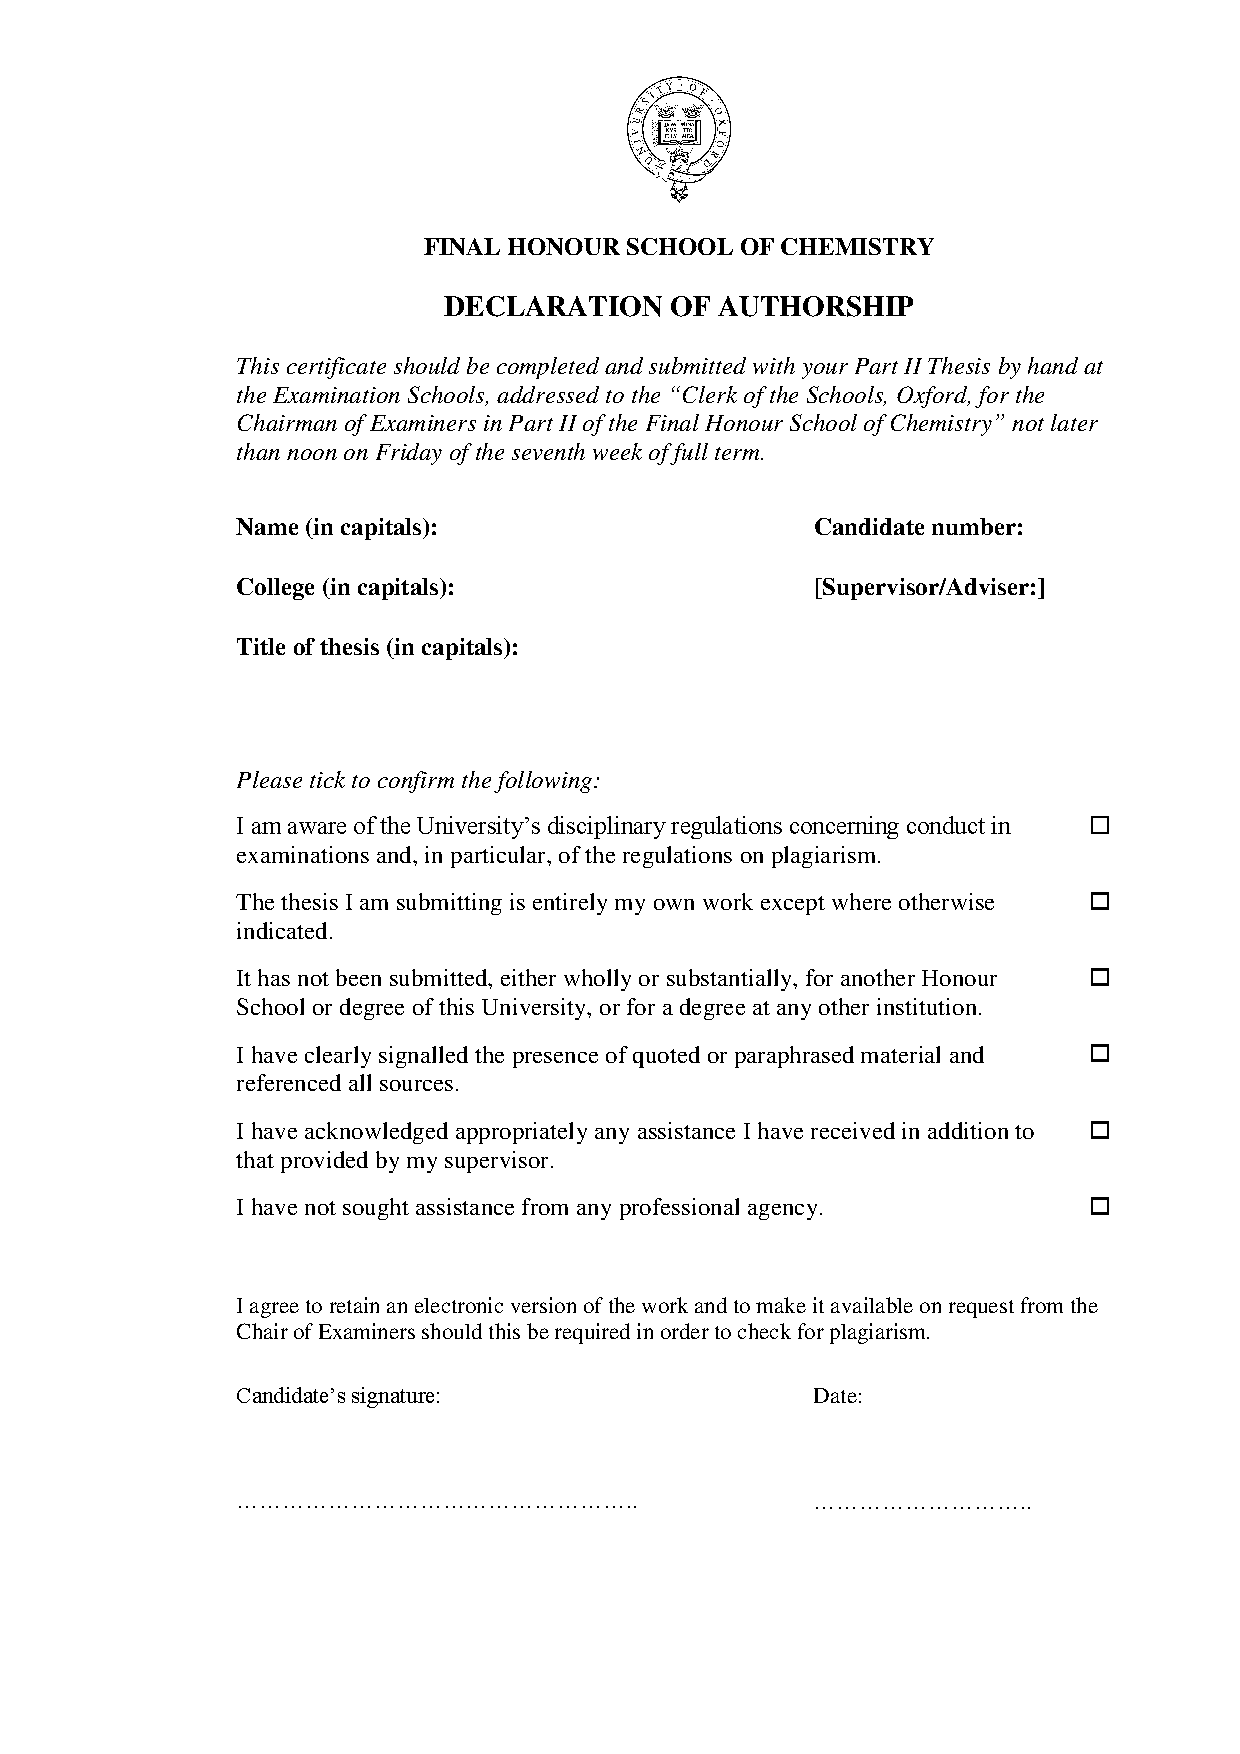
\includepdf[pages={1},draft=false,pagecommand={%
    \thispagestyle{plain}}]{./Other/DeclarationOfAuthorship}
\chapter{Acknowledgements}%

I would like to give thanks first and foremost to my project supervisor, Prof. Andrew Baldwin, who has provided me with bundles of support and wisdom throughout the year. Gogulan Karunanithy has aided me greatly with his expertise, especially with assistance in operating the PTCL's 600MHz NMR spectrometer. Satoshi Kishigami provided me with the $^{13}$CH$_3$-labelled samples used in this project, as well as $^{13}$CF$_3$-labelled samples, for which data acquisition is currently in progress. I would like to thank him for all our discussions relating to this aspect of the project. The entire Baldwin bunch have been a treat to spend time with over the year. As well as Andy, Gogs and Satoshi, I thank Virginia, Charlie, Magdeline, and Yixuan, for the numerous chats had over what was often a much-needed coffee.
% !TeX root = ./Report-Body.tex
\chapter{Abbreviations}%

% The abbreviations below are just examples. Remove those
% you don't need and include your own.

\begin{tabbing}
\hspace{0.5\parindent}\=\hspace{0.12\paperwidth}\=\+\kill
% You can manipulate the length {0.12\paperwidth} in the line
% above, as long as you don't intrude on any margins.
1D\> one dimensional\\
$\si{\angstrom}$\> angstrom(s) ($= \num{e-10} \si{\meter}$)\\
BWR\> Bloch-Wangness-Redfield\\
$^{\circ}$C\> Celsius\\
CPMG\> Carr-Purcell-Meiboom-Gill\\
CSA\> chemical shift anisotropy\\
d-DMSO\> deuterated dimethyl sulfoxide\\
d-glycerol\> deuterated glycerol\\
FID\> free induction decay\\
GHz\> gigahertz\\
HMQC\> heteronuclear multiple quantum coherence\\
HSQC\> heteronuclear single quantum coherence \\
Hz\> hertz\\
INEPT\> insensitive nuclei enhanced by polarisation transfer\\
K\> Kelvin\\
kDa\> kilodalton(s)\\
MDa\> megadalton(s)\\
MHz\> megahertz\\
NMR\> nuclear magnetic resonance\\
ns\> nanosecond(s)\\
PAF\> principle axis frame \\
PFG\> pulsed field gradient\\
ppm\> part(s) per million\\
ps\> picosecond(s)\\
rad\> radian(s)\\
rf\> radio-frequency\\
s\> second(s)\\
T\> tesla \\
TROSY\> transverse relaxation optimised spectroscopy
\end{tabbing}
\afterpage{\blankpage}
%%%%%
\hypersetup{pageanchor=true}
\mainmatter
% Report-Introduction.tex
% Simon Hulse
% simonhulse@protonmail.com
% Last Edited: Wed 27 Nov 2024 02:42:21 PM EST

% !TeX root = ./Report-Body.tex
\chapter{Introduction}

% Introduction text goes here
NMR Spectroscopy has been widely used for the study of biomolecular systems for over 70 years. The importance of the technique is evidenced by the fact that 2 Nobel Prizes in Chemistry have been awarded to pioneering figures in NMR (Ernst, 1991 and W\"{u}thrich, 2002). At present, it is the only experimental method that can measure both the structure and dynamics of biomolecules at atomic resolution on varying timescales.  Despite the unique information NMR can offer, there are certain features which limit the size of molecules that can feasibly be studied using it. As the size of the molecule increases, so too does the number of distinct chemical environments. This leads to increased spectral crowding, which can make the resolution of individual environments challenging. On top of this, the detectable magnetisation emanating from a molecule decays - via a process called \textit{relaxation} - more rapidly with increasing molecular size, which further reduces the resolving power of the experiment.\\
There are relatively few solved structures of biomolecules with molecular masses greater than 25 kDa using conventional techniques\cite{RN14}. Since 1997, development of \textit{Transverse Relaxation Optimised SpectroscopY} (TROSY) has enabled studies of molecules far larger. The original TROSY methodology was developed to target scalar-coupled $^{15}$N-$^1$H pairs commonly encountered in proteins\cite{RN15}. Additional TROSY techniques have been developed since, including methyl-TROSY, which involves probing proteins that have been selectively labelled with $^{13}$C methyl groups\cite{RN17, RN37}. This particular innovation allows biomolecules up to 1MDa to be studied\cite{RN16,RN35,RN36,RN22}. Despite this, the possibility of studying even larger systems, such as membrane-bound proteins, is of course desirable. The aim of this thesis is to explore possibilities for the development of such methods.\\
The use of $^{19}$F NMR may be a step towards extending the limits of bimolecular NMR. Whilst fluorine does not exist naturally within biomolecules, methods allowing the incorporation of $^{19}$F nuclei into proteins are emerging\cite{RN19}. The $^{13}$CF$_3$ group has certain features that make it a promising target for TROSY experiments. Firstly, the only $^{19}$F environments within a protein would come from the selectively inserted $^{13}$CF$_3$ labels, and therefore the resultant spectra would be far less crowded. Furthermore, the relaxation behaviour of $^{13}$CF$_3$ should vary substantially from $^{13}$CH$_3$, giving rise to the possibility of developing new NMR experiments that exploit this. The primary reason for this difference stems from the typically large $^{19}$F \textit{chemical shift anisotropy} (CSA), which arises due to a non-uniform electron density about the nucleus.\\
Whilst most NMR experiments can be adequately understood without a detailed appreciation of relaxation, this isn't the case for the TROSY experiments. The method is based on being highly selective about generating certain magnetisations that have favourable relaxation properties. The major focus of this thesis is to investigate the theory of relaxation in I$_3$S spin-systems, freely rotating as a part of larger molecules. Subsequently, validation of this theory via experimental means is attempted. Armed with a detailed understanding of I$_3$S relaxation phenomena, it will then become possible to devise an optimal $^{13}$CF$_3$-TROSY experiment.
\section{Basics of NMR and Relaxation} \label{sec1.1}
NMR experiments involve perturbing the magnetisation associated with an ensemble of spins away from its equilibrium state. This is achieved by the application of radio-frequency (rf) pulses. After such a perturbation is applied, the sample's net magnetisation will eventually return back to equilibrium, via relaxation. As a simple illustration of relaxation, one can consider how a sample's magnetisation evolves with time using the \textit{vector model}\cite{RN39}.\\ Consider an ensemble of isolated spin-$\frac{1}{2}$ nuclei, subjected to an external magnetic field, $\vec{B_0}$. The ensemble's net magnetisation, described by $\vec{M}$, will be parallel $\vec{B_0}$ at equilibrium. It is possible to rotate the net magnetisation of the sample into the plane perpendicular to the field direction. This is achieved by the application of a $\ang{90}$ rf pulse. Subsequently, $\vec{M}$ precesses about $\vec{B_0}$. However, the magnetisation does not precess within this perpendicular plane indefinitely. Instead, it gradually reverts back to its equilibrium position. Two separate relaxation rates are important to note:
\begin{itemize}
\item \textit{Longitudinal Relaxation}: the restoration of magnetisation along the field-direction (conventionally the z-direction), involving a change in population of spin states.
\item \textit{Transverse Relaxation}: a loss of coherence between spins, leading to depletion of magnetisation in the plane perpendicular to the field-direction. This does not require a change in population of the spin states.
\end{itemize}
\begin{figure}
\centering
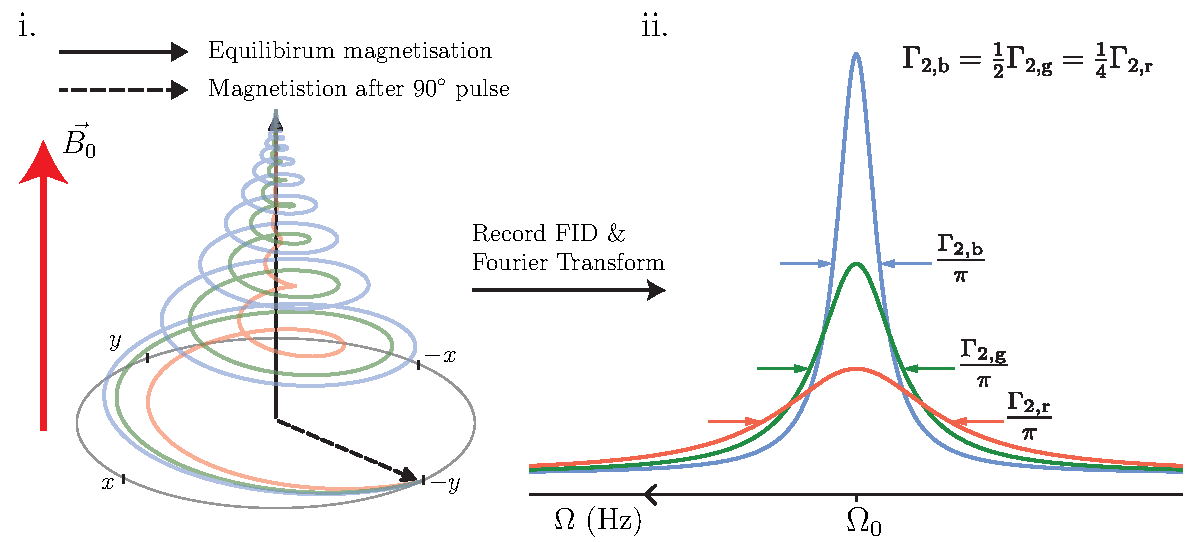
\includegraphics[scale=0.75]{./Figures/SimonsFigs/relaxation.pdf}
\caption{i. The time evolution of the bulk magnetisation for a system of spin-$\frac{1}{2}$ nuclei after a $\ang{90}$ pulse, described by the vector model. The relaxation of the magnetisation is parametrised by the longitudinal and transverse relaxation rate constants, $\Gamma_1$ and $\Gamma_2$. The three coloured spirals illustrate the time evolution of the magnetisation vector $\vec{M}$, with differing $\Gamma_2$ values, red having the largest value and blue having the smallest value. $\Gamma_1$ is kept constant for all cases. ii. The resulting signal, detected in the transverse plane, is Fourier Transformed to produce a spectrum, whose linewidth at half the peak's maximum intensity is $\frac{\Gamma_2}{\pi} \si{\myhertz}$}
\label{VecMod}
\end{figure}
These two processes typically occur at different rates in aqueous solution, parametrised by $\Gamma_1$ and $\Gamma_2$, respectively. Figure \ref{VecMod}.i illustrates how the magnetisation of an ensemble of spin-$\frac{1}{2}$ nuclei evolves with time, using the vector model. In the \textit{rotating frame}\cite{RN6}, the $x$-, $y$- and $z$-components of the magnetisation are described as follows:
\begin{equation}
M_x(t) = |\vec{M_0}| \sin(\Omega_0 t) e^{-\Gamma_2 t} \hspace{10pt} M_y(t) = -|\vec{M_0}| \cos(\Omega_0 t) e^{-\Gamma_2 t} \hspace{10pt} M_z(t) = |\vec{M_0}|\left(1 - e^{-\Gamma_1 t}\right)
\end{equation}
where $|\vec{M_0}|$ is the magnitude of the equilibrium magnetisation vector, and $\Omega_0$ is the offset frequency, equal to $\omega_0 - \omega_{\text{rf}}$. These expressions give rise to the spiral-like path that the magnetisation vector follows as it returns to equilibrium in Figure \ref{VecMod}.i. An NMR spectrometer is set up such that it is able to detect magnetisation transverse to the field direction. The signal it detects, called the free induction decay (FID), is Fourier Transformed to convert it from the time domain to the frequency domain. The resulting spectrum consists of a single peak, described by a Lorentzian function:
\begin{equation}
S(\Omega) = \text{Re}\left(\int \limits_0^{\infty} \underbrace{(M_x(t) + iM_y(t))}_{e^{i\Omega_0 t}}e^{-\Gamma_2 t}e^{i \Omega t} dt \right) = \frac{\Gamma_2}{\Gamma_2^2 + (\Omega_0 - \Omega)^2}
\end{equation}
The transverse relaxation rate constant, $\Gamma_2$ has a direct impact on the width of the peak, Figure \ref{VecMod}.ii. By noting that the maximum peak intensity occurs at $\Omega_0$,
\begin{equation}
\label{eq1.4}
S_{\text{max}}=S(\Omega_0)=\frac{1}{\Gamma_2} \therefore\  S_{\text{half-height}} = \frac{1}{2\Gamma_2}  \implies \Omega_{\text{half-height}} = \Omega_0 \pm \Gamma_2
\end{equation}
Hence, the width of a peak at half it's maximum is given by $2\Gamma_2\ \si{\radian\per\second} = \frac{\Gamma_2}{\pi}\ \si{Hz}$. The smaller $\Gamma_2$ is, the more intense and sharper the resultant spectral peaks will be.\\
Relaxation of the signal that is ultimately detected isn't the only factor that impacts the sensitivity of NMR experiments. Most NMR pulse sequences utilise several rf pulses, along with very precisely defined delay periods, on coupled spin systems. During the sequence, various forms of magnetisation are generated, which are used to provide detailed insights into molecular structure and function. But as the pulse sequence occurs, the magnetisation is constantly relaxing. This is particularly detrimental for large macromolecules that tumble very slowly in solution, as signal relaxation is typically very fast. By the time of acquisition, the manipulated magnetisation may have such a small intensity that it is indistinguishable from the stochastic noise inherent to all spectra. For these large systems, it is paramount to be highly selective in choosing the magnetisations that are allowed to evolve during the pulse sequence. This is precisely the aim of TROSY.
\section{An Overview of TROSY}
All TROSY experiments are devised with the same objective: to find a pulse sequence that takes at least some of the sample's magnetisation along a pathway where it is slowly relaxing at all times. I outline the key principles of two well-established TROSY techniques below. It is envisaged that combining traits of both of these experiments (notably dipolar/CSA interference from one, and dipolar/dipolar interference from the other) will yield a highly effective technique for targeting $^{13}$CF$_3$ moieties.
\subsection{$^{15}$N-$^1$H TROSY}
$^{15}$N-$^{1}$H spin pairs in proteins, excluding contributions from external spins, experience two major spin-relaxation mechanisms. The first of these is a dipolar interaction between the two nuclei. Secondly, there is a considerable $^{15}$N CSA. Both interactions average to zero during the measurement time-scale, but their fluctuations, induced by molecular tumbling, dominate relaxation. A one-dimensional $^1$H spectrum of a single $^{15}$N-$^{1}$H moiety will have a doublet structure as a result of scalar coupling between the nuclei. A doublet would also be observed if a 1D $^{15}$N spectrum was acquired. For each resonance in these doublets, the relaxation behaviour will differ. Notably, for resonances where the two major mechanisms reinforce each other, relaxation will be particularly fast, corresponding to a large $\Gamma_2$ value. Conversely, resonances in which these mechanisms act in opposite senses will relax slowly. As a result, the line widths of the peaks within each doublet will be different. Small, rapidly tumbling molecules do not show much discrepancy in peak widths within a doublet. By contrast, large, slowly tumbling molecules will typically exhibit drastic differences in peak widths, Figure \ref{NHTrosy}.\\
\begin{figure}
\centering
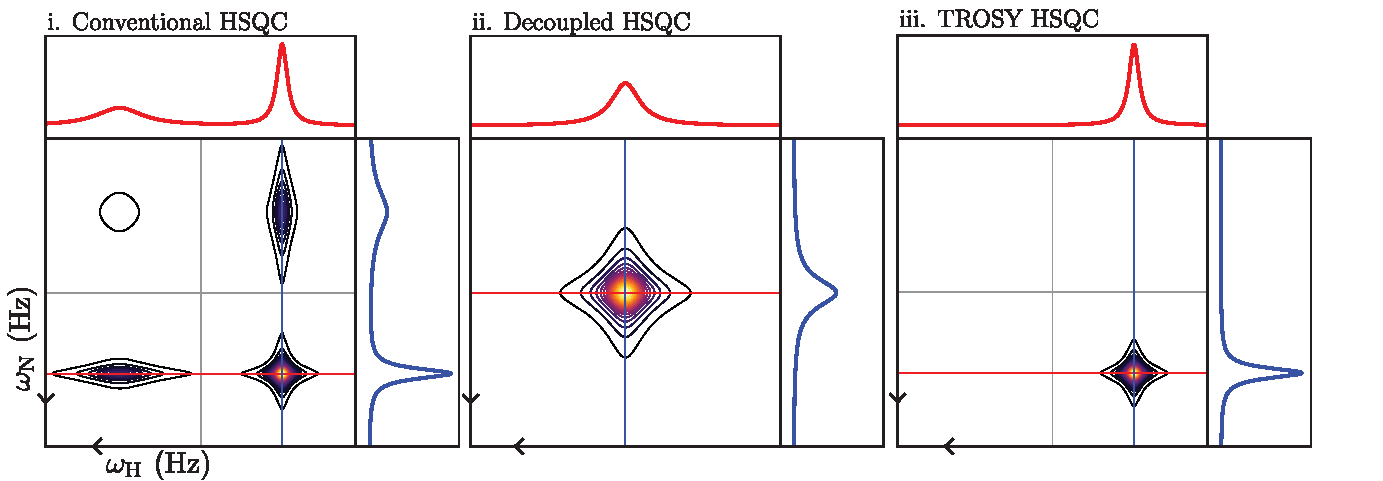
\includegraphics[scale=0.7]{./Figures/SimonsFigs/NHTrosy.pdf}
\caption{i. A HSQC spectrum of a typical $^{15}$N-$^1$H moiety in a large protein will feature peaks with highly pronounced linewidth differences, as a result of relaxation interference effects. ii. Decoupling such spectra produces peaks that originate from signal which has slowly and rapidly relaxing magnetisations mixed together, and can give rise to relatively low intensity peaks as a result. iii. In a $^{15}$N-$^1$H TROSY experiment, the use of phase-cycling discards signal that is rapidly relaxing, and retains the slowly relaxing signal only.}
\label{NHTrosy}
\end{figure}
A $^{15}$N-$^{1}$H Heteronuclear Single Quantum Coherence (HSQC) experiment produces a two-dimensional spectrum, with proton chemical shift on one axis, and $^{15}$N shift on the other. The resultant peaks provide correlations between scalar coupled $^{15}$N-$^{1}$H pairs. In the $^{15}$N-$^1$H TROSY experiment, selection of the peak corresponding to slowly relaxing magnetisaions in both dimensions is achieved via phase-cycling. The result is a loss of total signal obtained from an NMR experiment, though the signal retained gives rise to an intense, sharp line, Figure \ref{NHTrosy}.iii. For sufficiently slowly tumbling molecules, with inherently fast-relaxing magnetisations, intensity gains relative to conventional decoupled spectra are achieved using this methodology.
\subsection{Methyl TROSY}
\begin{figure}
\centering
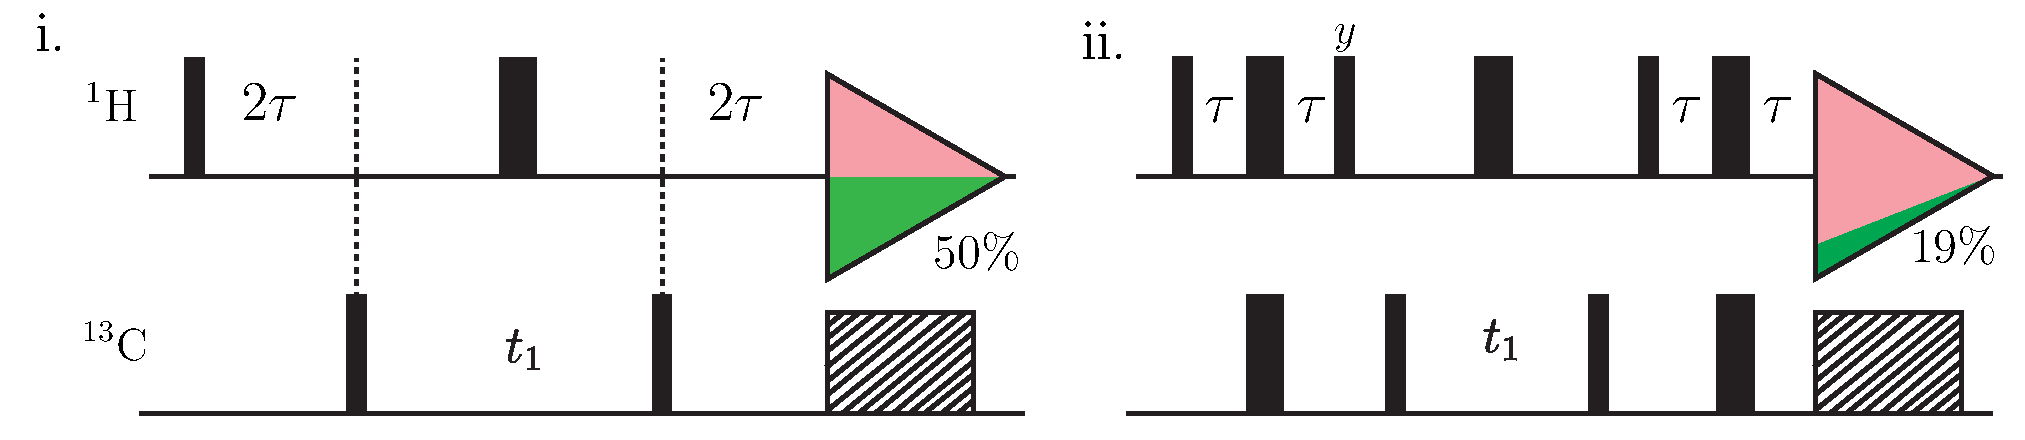
\includegraphics[scale=0.4]{./Figures/SimonsFigs/HSQCHMQC.pdf}
\caption{Simplified pulse sequence diagrams for a HMQC and a HSQC experiments (i. and ii. respectively). Narrow (Wide) bars represent $\ang{90}$ ($\ang{180}$) rf pulses, applied to the nucleus specified. The detected signal (FID) is represented by a triangle. During detection of the FID, heteronuclear decoupling (represented by a dashed box) is applied to the $^{13}$C nucleus to remove multiplet structures. The optimum value of the time $\tau$ is $\frac{1}{4J_{\text{CH}}}$, where $J_{\text{CH}}$ is the $^{13}$C-$^1$H scalar coupling constant.}
\label{HSQCHMQC}
\end{figure}
Within the $^{13}$CH$_{3}$ moiety, relaxation is dominated by numerous dipolar interactions (those being $^{13}$C-$^1$H and $^1$H-$^1$H dipolar interactions). The HSQC experiment is very poor for the study of methyl groups in large macromolecules, as during the pulse sequence, rapidly and slowly magnetisations are heavily mixed via the application of numerous $\ang{90}$ rf pulses. The Heteronuclear Multiple Quantum Coherence (HMQC) experiment, remarkably, is an optimal TROSY experient for methyl groups\cite{RN17, RN37}, Figure \ref{HSQCHMQC}. For the case of large macromolecular systems, on the order of hundred of $\si{\kilo\dalton}$ and above, calculations show that 50\% of the total signal detected from a HMQC experiment originates from magnetisation that is slowly relaxing throughout the pulse sequence. This is the case for only 19\% of the detected signal in a HSQC experiment\cite{RN17}.
\section{Thesis Outline}
In the the next chapter of this thesis, models used to describe relaxation phenomena in I$_3$S spin-systems are derived, which are extensions of current models used. The models presented have the benefit of being appropriate for all molecular size regimes. As well as this, they incorporate all appropriate relaxation mechanisms, including the I-spin CSA, which is crucial for the case of $^{13}$CF$_3$ spin systems. Following a derivation of the theory, theoretical calculations of selected relaxation rates are presented, and analysed in detail. From this, predictions on the viability of a $^{13}$CF$_3$ moiety as a good candidate for a TROSY methodology are made. Finally, some experimental relaxation studies on a system intended to mimic the behaviour of biomolecules are presented, in attempts to validate our proposed theory.

% !TeX root = ./Report-Body.tex
\renewcommand{\arraystretch}{0.6}
\setlength\arraycolsep{2pt}
\renewcommand{\thefootnote}{\fnsymbol{footnote}}
\chapter{Derivation of Theory}
In order to gain a detailed, quantitative understanding of relaxation, it is necessary to delve into quantum mechanics. In this chapter, Bloch-Wangness-Redfield (BWR) Theory is introduced. A novel model specifically devised to describe the relaxation of a methyl or trifluoromethyl group within a molecule is presented. By establishing this theory, which incorporates both dipolar and CSA influences, it will become possible to establish which magnetisations are desirable to target during a $^{13}$CF$_3$ TROSY experiment.
\section{Spin Ensembles and the Density Matrix}
A nuclear spin, just like any other quantum system, is described by a wavefunction, $\ket{\Psi}$, which provides all discernible information about it. Any spin within an NMR sample will possess a wavefunction that consists of a linear combination of its basis eigenkets. For a spin-$\frac{1}{2}$ nucleus, this wavefunction takes a particularly simple form if we expand it in terms of the eigenkets of the $\hat{I}_z$ angular momentum operator:
\begin{equation}
\ket{\Psi}=c_{\alpha}\ket{\alpha}+c_{\beta}\ket{\beta}
\end{equation}
To describe NMR experiments, in which the system being studied comprises a very large ensemble of spins, in a mixed state, it is common practice to consider the \textit{density operator}, defined by:
\begin{equation}
\hat{\rho}=\overline{\ket{\Psi}\bra{\Psi}}
\end{equation}
where the overbar represents the average value for the entire ensemble\footnote{Note that in following sections, the overbar indicating ensemble averaging will sometimes be dropped for convenience, however this is implied throughout.}. The matrix representation of $\hat{\rho}$ features elements $\rho_{ba}=\overline{c_a^*c_b}$. For an ensemble of isolated spin-$\frac{1}{2}$ nuclei, $\hat{\rho}$ is given by:
\begin{equation}
\hat{\rho} = \mqty(\overline{\ket{\alpha}\bra{\alpha}} & \overline{\ket{\alpha}\bra{\beta}} \\ \overline{\ket{\beta}\bra{\alpha}} & \overline{\ket{\beta}\bra{\beta}}) = \mqty(\overline{c_{\alpha}^*c_{\alpha}} & \overline{c_{\beta}^*c_{\alpha}} \\ \overline{c_{\alpha}^*c_{\beta}} & \overline{c_{\beta}^*c_{\beta}})
\end{equation}
The ensemble-averaged expectation value of an observable corresponding to the operator $\hat{O}$, is given by:
\begin{equation}
\label{ExpVal}
\overline{\expval{\hat{O}}} = \text{Tr}\left[{\hat{\rho}\hat{O}}\right]
\end{equation}
The crux of NMR experiment analysis is to determine the time evolution of the density matrix during a pulse sequence. It then becomes possible to evaluate the expectation values of observables that are of interest, using \ref{ExpVal}.\\
It is common to represent the density operator as a linear combination of time-independent operators that form a complete basis, with time-dependent coefficients:
\begin{equation}
\hat{\rho} = \sum \limits_i c_i (t) \hat{O}_i
\end{equation}
where, for an ensemble of isolated spin-$\frac{1}{2}$ nuclei, the matrix representation of each operator, $\hat{O}_i$, is defined by:
\begin{equation}
\hat{O}_i = \mqty(\mel{\alpha}{\hat{O}_i}{\alpha} & \mel{\alpha}{\hat{O}_i}{\beta} \\ \mel{\beta}{\hat{O}_i}{\alpha} & \mel{\beta}{\hat{O}_i}{\beta})
\end{equation}
Two bases are conventionally used to describe an ensemble of spins, each one possessing four operators for an ensemble of isolated spin-$\frac{1}{2}$ nuclei. These are the Cartesian basis and the Single-element basis. Definitions of all the operators in these bases are defined as follows:\\
Cartesian basis:
\begin{equation}
\frac{1}{2}\hat{E} = \mqty(\frac{1}{2} & 0 \\ 0 & \frac{1}{2}) \hspace{20pt} \hat{I}_x = \mqty(0 & \frac{1}{2} \\ \frac{1}{2} & 0) \hspace{20pt} \hat{I}_y = i\mqty(0 & \frac{1}{2} \\ -\frac{1}{2} & 0) \hspace{20pt} \hat{I}_z = \mqty(\frac{1}{2} & 0 \\ 0 & -\frac{1}{2})
\end{equation}
Single-element basis:
\begin{equation}
\hat{I}^{\alpha} = \frac{1}{2} \hat{E} + \hat{I}_z \hspace{20pt} \hat{I}^{\beta} = \frac{1}{2} \hat{E} - \hat{I}_z \hspace{20pt} \hat{I}^+ = \hat{I}_x + i\hat{I}_y \hspace{20pt} \hat{I}^- = \hat{I}_x - i\hat{I}_y 
\end{equation}
The complete density matrix of an ensemble of isolated spin-$\frac{1}{2}$ nuclei is therefore given by:
\begin{equation}
\hat{\rho} = \frac{1}{2} c_E \hat{E} + c_x \hat{I}_x + c_y \hat{I}_y + c_z \hat{I}_z = c_{\alpha} \hat{I}^{\alpha} + c_{\beta} \hat{I}^{\beta} + c_+ \hat{I}^+ + c_- \hat{I}^-
\end{equation} 
\subsection{Multi-spin Systems}
To construct wave functions describing a system of multiple scalar-coupled spins, direct (Kronecker) products of the relevant single-spin wavefunctions are taken. For an N-spin system:
\begin{equation}
\ket{\Psi_{N\text{-spin}}} = \ket{\psi_1} \otimes \ket{\psi_2} \otimes ... \otimes \ket{\psi_N}
\end{equation}
In general, the density matrix describing an ensemble of $N$ scalar-coupled spin-$\frac{1}{2}$ nuclei is $2^N \times 2^N$ in dimension, and described by a linear combination of $4^N$ operators. These operators are formed by taking Kronecker products of the single spin operators descried above.
The spin systems of primary interest in this thesis ($^{13}$CH$_3$ and $^{13}$CF$_3$) consist of 4 spin-$\frac{1}{2}$ nuclei. As such, a complete density matrix describing these systems is $16 \times 16$ in dimension, and composed of a linear combination of $256$ product operators.
\section{Time Dependence of the Density Matrix}
The time-dependence of the density operator, under the influence of a Hamiltonian, $\hat{H}$, is described by the Liouville-von Neumann equation\cite{RN39}:
\begin{equation}
\dv{\hat{\rho}}{t}=-i\comm{\hat{H}}{\hat{\rho}}
\end{equation}
A common treatment of the Hamiltonian in the context of spin dynamics is to assume that it is composed of two separate parts:
\begin{equation}
\begin{split}
\hat{H} (t) &= \hat{H}_0 + \hat{H}_1 (t) \\
\therefore \dv{\hat{\rho} (t)}{t} &= -i \left\lbrace\comm{\hat{H}_0}{\hat{\rho (t)}} + \comm{\hat{H}_1 (t)}{\hat{\rho (t)}}\right\rbrace
\end{split}
\end{equation}
where $\hat{H}_0$ describes all the time-independent contributions to the Hamiltonian, and $\hat{H}_1 (t)$ describes the time-dependent contributions, arising from random fluctuations in local magnetic fields within the sample. It should be noted that the time-averaged value of $\hat{H}_1 (t)$, given by $\overline{\hat{H}_1(t)}$ is 0. As such, $\hat{H}_1 (t)$ has no bearing on the position or number of peaks in spectra, though it plays a key role in the relaxation of nuclear spin systems.
The most widely utilised theory for the study of nuclear spin relaxation was devised by Bloch, Wangsness and Redfield\cite{RN23,RN13}. The key result of BWR theory is the following expression describing the time-dependence of the density matrix: 
\begin{equation}
\label{superoperator}
\begin{gathered}
\pdv{\hat{\rho}(t)}{t} = -i \comm{\hat{H}_0}{\hat{\rho} (t)} - \hat{\hat{\Gamma}}(\hat{\rho} (t) - \hat{\rho}_{\text{eq}}) \\
\hat{\hat{\Gamma}} = \int \limits_0^{\infty} \overline{\comm{\hat{H}_1 (t)^{\dagger}}{\comm{e^{-i \hat{H}_0 \tau} \hat{H}_1 (t - \tau)  e^{i \hat{H}_0 \tau}}{}}} d \tau
\end{gathered}
\end{equation}
where $\hat{\hat{\Gamma}}$ is the \textit{relaxation superoperator},  and $\hat{\rho}_{\text{eq}}$ is the density matrix of the ensemble in its equilibrium state. A derivation of this result is outlined in Appendix A. The matrix form of $\hat{\hat{\Gamma}}$ comprises elements $\Gamma_{rs}$ defined by:
\begin{equation}
\Gamma_{rs} = \frac{\mel{\hat{\rho}_s}{\hat{\hat{\Gamma}}}{\hat{\rho}_r}}{\sqrt{\bra{\hat{\rho}_r} \ket{\hat{\rho}_r} \bra{\hat{\rho}_s} \ket{\hat{\rho}_s}}}
\end{equation}
\section{Hamiltonians in Relaxation}
It is necessary to derive the form of $\hat{H}_1(t)$, the operator which describes the stochastically fluctuating local interactions within an NMR sample. Hamiltonians that describe the relevant interactions which induce relaxation need to be established. Common examples of such interactions include the dipolar interaction, the chemical shift anisotropy, and the quadrupolar interaction. This thesis focusses solely on spin-$\frac{1}{2}$ nuclei. As such, the quadrupolar interaction, which only applies when considering nuclei that are spin-$1$ or higher, will not be considered. Following this, we must perform rotations on the Hamiltonian, in order to imitate the motion of the molecule in solution, to work out their effects on relaxation.
\subsection{Hamiltonians in Spin Dynamics}
It is necessary to consider the different contributions to the stochastic Hamiltonian, $\hat{H}_1 (t)$, in order to describe relaxation phenomena successfully. Fortunately, there is a general framework which can be applied to all Hamiltonians relevant to spin-relaxation. Any such Hamiltonian may be expressed as follows:
\begin{equation}
\hat{H}=\vec{I}^\intercal \cdot \hat{A} \cdot \vec{S}
\end{equation}
$\vec{I}$ and $\vec{S}$ are vectors which describe the two interacting entities. These would represent two distinct spins in the case for the dipolar interaction. When considering the CSA, they would represent a spin and the external magnetic field, respectively. $\hat{A}$ is a second rank tensor that characterises the interaction. In a Cartesian axis system, the explicit form of the Hamiltonian is defined by:
\begin{equation}
\hat{H} = \mqty(\hat{I}_x & \hat{I}_y & \hat{I}_z) \mqty(A_{xx} & A_{xy} & A_{xz} \\ A_{yx} & A_{yy} & A_{yz} \\ A_{zx} & A_{zy} & A_{zz}) \mqty(\hat{S}_x \\ \hat{S}_y \\ \hat{S}_z)
\end{equation}
The values of the elements within the tensor $\hat{A}$ are dependent on the co-ordinate system in which we cast it. The simplest co-ordinate system possible is such that the interaction tensor is diagonal, which is known as its \textit{Principal Axis Frame} (PAF):
\begin{equation}
\label{PAFtensor}
\hat{A}_{\text{PAF}} = \mqty(A_{11} & 0 & 0 \\ 0 & A_{22} & 0 \\ 0 & 0 & A_{33})
\end{equation}
It is possible to split \ref{PAFtensor}, by defining three properties of the tensor; the \textit{isotropy}, the \textit{anisotropy}, and the \textit{asymmetry}:
\begin{equation}
\label{IsoAnisoAsymm}
A_{\text{iso}} = \frac{1}{3} (A_{11} + A_{22} + A_{33}) \hspace{15pt} A_{\text{aniso}} = \frac{1}{3} (A_{33} - A_{11}) \hspace{15pt} A_{\text{asymm}} = \frac{A_{22} - A_{11}}{A_{33} - A_{11}}
\end{equation}
Using the quantities defined in \ref{IsoAnisoAsymm}, $\hat{A}_{\text{PAF}}$ can be written as:
\begin{equation}
\label{PAFtensor_broken}
\hat{A}_{\text{PAF}} = A_{\text{iso}} \mqty(\imat{3}) + A_{\text{aniso}} \mqty(-1 & 0 & 0 \\ 0 & -1 & 0 \\ 0 & 0 & 2) + A_{\text{asymm}} A_{\text{aniso}} \mqty(1 & 0 & 0 \\ 0 & -2 & 0 \\ 0 & 0 & 1)
\end{equation}  
Whilst the PAF is the most convenient way to express a particular Hamiltonian, it necessary to express the Hamiltonian in terms of a set of co-ordinates that rotate relative to the internal co-ordinates of the molecule. We call such a system the \textit{Laboratory Frame}. However, before converting to the laboratory frame, establishment of the fixed orientations of the interaction tensors relative to each other is required. Doing this brings the system into the \textit{Molecular Frame}. In the following section, the necessary theory of rotations required to achieve such transformations is outlined. 
\subsection{Relevant Theory of Rotations}
A general rotation, by Euler angles $(\alpha$, $\beta$, $\gamma)$, applied to a Hamiltonian is given by:
\begin{equation}
\hat{H}_{\text{rot}} = \hat{\hat{R}}(\alpha, \beta, \gamma)[\vec{I}^{\intercal}\cdot\hat{A}\cdot\vec{S}] = \vec{I}^{\intercal} \cdot \hat{R}(\alpha, \beta, \gamma) \hat{A} \hat{R}^{-1}(\alpha, \beta, \gamma) \cdot \vec{S}
\end{equation}
The $z$-$y$-$z$ convention is commonly used, where an object is first rotated by the angle $\gamma$ about the $z$-axis, then by the angle $\beta$ about the $y$-axis, and finally by the angle $\alpha$ about the $z$-axis. As such, $\hat{R}(\alpha, \beta, \gamma)$ is defined by:
\begin{equation}
\hat{R}(\alpha, \beta, \gamma) = \mqty(\cos \alpha & -\sin \alpha & 0 \\ \sin \alpha & \cos \alpha & 0 \\ 0 & 0 & 1) \mqty(\cos \beta & 0 & -\sin \beta \\ 0 & 1 & 0 \\ \sin \beta & 0 & \cos \beta) \mqty(\cos \gamma & -\sin \gamma & 0 \\ \sin \gamma & \cos \gamma & 0 \\ 0 & 0 & 1)
\end{equation}
Whilst performing rotations on the PAF Hamiltonian in the form already presented is perfectly valid, these rotations will be far more manageable by changing the basis of operators that are used to describe it. The basis of choice is that of the \textit{irreducible spherical tensor operators}. There are 5 2$^{\text{nd}}$-rank spherical tensor operators, $\hat{T}_k^{(2)}$, where $k$ takes the values $-2$ to $2$ in integer steps. 
The result of applying a general rotation by Euler angles $(\alpha$, $\beta$, $\gamma)$ on a spherical tensor operator of rank 2 is as follows:
\begin{equation}
\hat{\hat{R}}(\alpha, \beta, \gamma) \hat{T}_{k}^{(2)} = \sum \limits_{k{\prime} = -2}^2 \mathfrak{D}_{k{\prime},k}^{(2)}(\alpha, \beta, \gamma) \hat{T}_{k{\prime}}^{(2)}
\end{equation}
Where $\mathfrak{D}_{k{\prime},k}^{(2)}(\alpha, \beta, \gamma)$ are the elements of the the $\text{2}^{\text{nd}}$-rank Wigner D-Matrix. The elements of this matrix are related to those of the reduced $\text{2}^{\text{nd}}$-rank Wigner Matrix, $d_{k{\prime},k}^{(2)}(\beta)$, according to:
\begin{equation}
\mathfrak{D}_{k{\prime},k}^{(2)}(\alpha, \beta, \gamma) = e^{-i k{\prime} \alpha} d_{k{\prime},k}^{(2)}(\beta) e^{-i k \gamma}
\end{equation}
Where the reduced $\text{2}^{\text{nd}}$-rank Wigner Matrix is defined as follows:
\begin{equation}
\label{RedWignerMatrix}
\mqty(\frac{(1 + \cos\beta)^2}{4} & -\frac{(1+\cos\beta)\sin\beta}{2} & \sqrt{\frac{3}{8}}\sin^2\beta & -\frac{(1-\cos\beta)\sin\beta}{2} & \frac{(1-\cos\beta)^2}{4} \\ \frac{(1+\cos\beta)\sin\beta}{2} & \frac{cos\beta - 1}{2} + \cos^2\beta & -\sqrt{\frac{3}{8}}\sin2\beta & \frac{\cos\beta + 1}{2} - \cos^2\beta & -\frac{(1 - \cos\beta)\sin\beta}{2} \\ \sqrt{\frac{3}{8}}\sin^2\beta & \sqrt{\frac{3}{8}}\sin2\beta & \frac{3\cos^2\beta - 1}{2} & -\sqrt{\frac{3}{8}}\sin2\beta & \sqrt{\frac{3}{8}}\sin^2\beta \\ \frac{(1 - \cos\beta)\sin\beta}{2} & \frac{\cos\beta + 1}{2} - \cos^2\beta & \sqrt{\frac{3}{8}}\sin2\beta & \frac{\cos\beta - 1}{2} + \cos^2\beta & -\frac{(1 + \cos\beta)\sin\beta}{2} \\ \frac{(1 - \cos\beta)^2}{4} & \frac{(1 - \cos\beta)\sin\beta}{2} & \sqrt{\frac{3}{8}}\sin^2\beta & \frac{(1 + \cos\beta)\sin\beta}{2} & \frac{(1 + \cos\beta)^2}{4})
\end{equation}
Some of the spherical tensor operators consist of sums of linear combinations of operators. It will become highly beneficial when deriving an expression for $\hat{\hat{\Gamma}}$ to split these particular tensors into terms containing single operators, as follows:
\begin{equation}
\hat{T}_k^{(2)} = \sum \limits_n \hat{T}_{k,n}^{(2)}
\end{equation}
The full set of $\hat{T}_{k,n}^{(2)}$ terms are given in Table \ref{SphericalOperators}.\\
\begin{table}[]
\centering
\begin{tabular}{l|lll}
       & $n = 1$ & $n = 2$ & $n = 3$ \\ \hline
$k=-2$ & $\frac{1}{2} \hat{I}^{-} \hat{S}^{-}$      & -       & -       \\
$k=-1$ & $\frac{1}{2} \hat{I}_z \hat{S}^{-}$      & $\frac{1}{2} \hat{I}^{-} \hat{S}_{z}$      & -       \\
$k=0$  & $\sqrt{\frac{2}{3}} \hat{I}_{z} \hat{S}_{z}$      & $-\frac{1}{4} \sqrt{\frac{2}{3}} \hat{I}^{+} \hat{S}^{-}$      & $-\frac{1}{4} \sqrt{\frac{2}{3}} \hat{I}^{-} \hat{S}^{+}$      \\
$k=1$  & $-\frac{1}{2} \hat{I}_z \hat{S}^{+}$      & $-\frac{1}{2} \hat{I}^{+} \hat{S}_z$      & -       \\
$k-2$  & $\frac{1}{2} \hat{I}^{+} \hat{S}^{+}$      & -       & -      
\end{tabular}
\caption{The full set of terms, $T_{k,n}^{(2)}$, that make up the spherical tensor operators, $\hat{T}_k^{(2)}$. The range of values $n$ takes depends on the value of $k$. For $k = \pm 2$, $n=1$ only. For $k = \pm 1$, $n=1, 2$. Finally, for $k = 0$, $n=1, 2, 3$.}
\label{SphericalOperators}
\end{table}
\subsection{Transforming a Hamiltonian into the Molecular Frame}
With this framework for rotations established, we now look to express $\hat{H}_{\text{PAF}}$ in terms of spherical tensor operators. Using the definition of $\hat{A}_{\text{PAF}}$ in \ref{PAFtensor_broken}, $\hat{H}_{\text{PAF}}$ takes the following form:
\begin{equation}
\begin{split}
\hat{H}_{\text{PAF}} = &\underbrace{A_{\text{iso}}\left(\hat{I}_x \hat{S}_x + \hat{I}_y \hat{S}_y + \hat{I}_z \hat{S}_z\right)}_{\tiny\textcircled{1}}  + \underbrace{A_{\text{aniso}}\left(-\hat{I}_x \hat{S}_x - \hat{I}_y \hat{S}_y + 2\hat{I}_z \hat{S}_z\right)}_{\tiny\textcircled{2}} \\ &+ \underbrace{A_{\text{aniso}} A_{\text{asymm}} \left(\hat{I}_x \hat{S}_x - 2\hat{I}_y \hat{S}_y + \hat{I}_z \hat{S}_z\right)}_{\tiny\textcircled{3}}
\end{split}
\end{equation}
By noting the relations $\hat{I}_x \hat{S}_x = \frac{1}{4}\left(\hat{I}^+ + \hat{I}^-\right)\left(\hat{S}^+ + \hat{S}^-\right)$ and \\$\hat{I}_y \hat{S}_y = -\frac{1}{4}\left(\hat{I}^+  - \hat{I}^-\right)\left(\hat{S}^+ - \hat{S}^-\right)$, the components of the Hamiltonian that are affected by rotation\footnote{The isotropic component of a Hamiltonian, \textcircled{1}, is invariant to rotation, and as such does not contribute to relaxation. It is incorporated in the time-independent Hamiltonian, $\hat{H}_0$.} can be re-expressed as follows:
\begin{equation}
\begin{split}
&\textcircled{2} =\sqrt{6}A_{\text{aniso}}\hat{T}_0^{(2)} \\
&\textcircled{3} = \frac{1}{2} A_{\text{aniso}} A_{\text{asymm}} \left(3 (\hat{T}_2^{(2)} + \hat{T}_{-2}^{(2)}) - \sqrt{6} \hat{T}_0^{(2)} \right)
\end{split}
\end{equation}
In this thesis it is assumed that all contributions to $\hat{H}_1 (t)$ solely have an anisotropic contribution\footnote{A useful simplification arises by assuming that the interaction tensors are axially symmetric (i.e. $A_{\text{asymm}} = 0$). A rotation of an axially symmetric tensor, aligned along the $z$-axis, about the $z$-axis has no effect. We therefore only require two angles to describe the rotation of such tensors, $\beta$ and $\alpha$. These correspond to the polar ($\theta$) and azimuthal ($\phi$) angles used in the spherical polar co-ordinate system.}, such that:
\begin{equation}
\hat{H}_{\text{PAF}} = \hat{H}_{\text{iso}} + \sqrt{6} A_{\text{aniso}}\hat{T}_0^{(2)}
\end{equation}
In order to bring the Hamiltonian into the molecular frame, a time-independent rotation, $\Omega$, is applied to it: 
\begin{equation}
\label{MolFrameHam}
\hat{H}_{\text{mol}} = \hat{H}_{\text{iso}} + \sqrt{6} A_{\text{aniso}} \sum \limits_{k = -2}^2 \mathfrak{D}_{k,0}^{(2)}(\Omega) \sum \limits_n \hat{T}_{k,n}^{(2)}
\end{equation}
where $\Omega = (\alpha, \beta)$ 
\subsection{Bringing a Hamiltonian into the Laboratory Frame}
A general interaction Hamiltonian in the Laboratory frame is generated by rotating \ref{MolFrameHam} in a way that mimics the motion of the system of interest. This is achieved by applying time-dependent rotations to the Hamiltonian. If a single 'type' of motion occurs, the Laboratory Frame Hamiltonian takes the form:
\begin{equation}
\label{LabFrameHamIso}
\hat{H}_{\text{Lab}} = \hat{H}_{\text{iso}} + \sqrt{6}A_{\text{aniso}} \sum \limits_{m = -2}^2 \sum \limits_{k = -2}^2  \mathfrak{D}_{m,k}^{(2)}(t) \mathfrak{D}_{k,0}^{(2)} (\Omega) \sum_n\hat{T}_{k,n}^{(2)}
\end{equation}
This form is appropriate for describing a Hamiltonian following the global rotation of the molecule, with the absence of any locally defined motion affecting it. For example, $^{15}$N-$^1$H pairs in the amide backbone can be adequately described in this fashion. In contrast, describing the motion of I$_3$S spin systems, such as methyl groups, is not appropriate using \ref{LabFrameHamIso}. In this case, the methyl group rotates rapidly about its threefold symmetry axis, whilst also following the global motion of the molecule as a whole. An extra rotation to account for this methyl rotation is necessary. To consider the form of such a Hamiltonian, we start, again, at \ref{MolFrameHam}. To describe the motion of the I$_3$S moiety, this Hamiltonian is operated on by a rotation, $\hat{\hat{R}}_{\text{methyl}}$: 
\begin{equation}
\hat{H}_{\text{Lab}} = \hat{H}_{\text{iso}} + \sqrt{6} A_{\text{aniso}} \hat{\hat{R}}_{\text{methyl}} \sum \limits_{k = -2}^2 \mathfrak{D}_{k,0}^{(2)}(\Omega) \sum \limits_n \hat{T}_{k,n}^{(2)}
\end{equation}
\begin{figure}
\centering
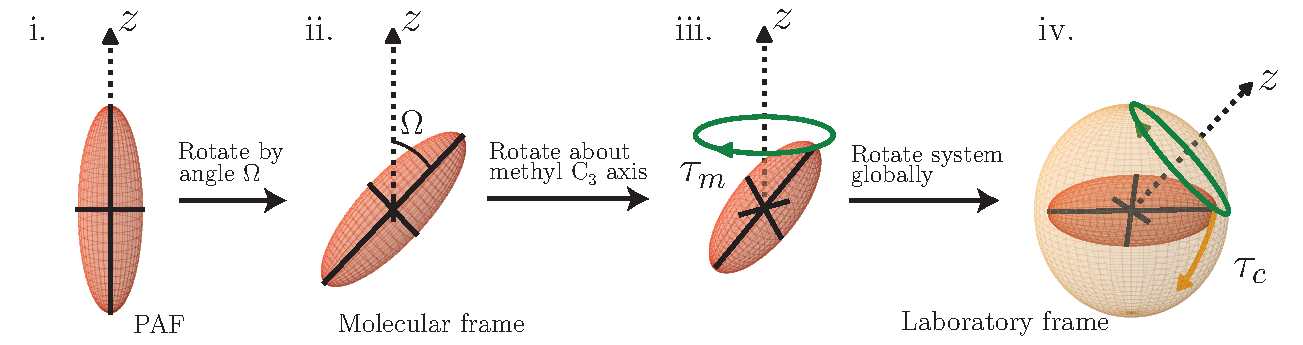
\includegraphics[scale=0.65]{./Figures/SimonsFigs/Rotations.pdf}
\caption{The sequence of rotations applied to the interaction tensors using the methyl rotation model. i. The tensor is initially aligned along the $z$-axis of the PAF. ii. It is then rotated into the molecular frame by the angle $\Omega(\alpha,\beta)$. iii. It is then allowed to rotate about the $z$-axis, which is defined to be the threefold rotation axis of the methyl group, characterised by correlation time $\tau_{\text{m}}$. iv. Finally, the whole system is allowed to undergo spherical isotropic motion, characterised by correlation time $\tau_{\text{c}}$.}
\label{Rotations}
\end{figure}
The $z$-axis is assumed to be the methyl rotation axis. As a result,  the angle $\beta$, which describes rotation about the $y$-axis, is set to $0$. Only diagonal elements of the Wigner D-Matrix which describe rotation about the methyl axis will be non-zero, which can be seen by inspecting \ref{RedWignerMatrix}. Incorporating methyl rotation, and subsequently global tumbling into the Hamiltonian therefore yields:
\begin{equation}
\hat{H}_{\text{Lab}} = \hat{H}_{\text{iso}} + \sqrt{6} A_{\text{aniso}} \hat{\hat{R}}_{\text{c}} \hat{\hat{R}}_{\text{m}} \sum \limits_{k = -2}^2 \mathfrak{D}_{k,0}^{(2)}(\Omega) \sum \limits_n \hat{T}_{k,n}^{(2)}
\end{equation}
where the rotation matrices, $\hat{\hat{R}}_{\text{m}}$  and $\hat{\hat{R}}_{\text{c}}$, which correspond to local methyl rotation and global tumbling respectively, are given by:
\scriptsize
\begin{equation}
\hat{\hat{R}}_{\text{m}} = \mqty(\mathfrak{D}_{-2,-2}^{(2) \text{m}} & 0 & 0 & 0 & 0 \\ 0 & \mathfrak{D}_{-1,-1}^{(2) \text{m}} & 0 & 0 & 0 \\ 0 & 0 & \mathfrak{D}_{0,0}^{(2) \text{m}} & 0 & 0 \\ 0 & 0 & 0 & \mathfrak{D}_{1,1}^{(2) \text{m}} & 0 \\ 0 & 0 & 0 & 0 & \mathfrak{D}_{2,2}^{(2) \text{m}}),
\hat{\hat{R}}_{\text{c}} = \mqty(\mathfrak{D}_{-2,-2}^{(2) \text{c}} & \mathfrak{D}_{-2,-1}^{(2) \text{c}} & \mathfrak{D}_{-2,0}^{(2) \text{c}} & \mathfrak{D}_{-2,1}^{(2) \text{c}} & \mathfrak{D}_{-2,2}^{(2) \text{c}} \\ \mathfrak{D}_{-1,-2}^{(2) \text{c}} & \mathfrak{D}_{-1,-1}^{(2) \text{c}} & \mathfrak{D}_{-1,0}^{(2) \text{c}} & \mathfrak{D}_{-1,1}^{(2) \text{c}} & \mathfrak{D}_{-1,2}^{(2) \text{c}} \\ \mathfrak{D}_{0,-2}^{(2) \text{c}} & \mathfrak{D}_{0,-1}^{(2) \text{c}} & \mathfrak{D}_{0,0}^{(2) \text{c}} & \mathfrak{D}_{0,1}^{(2) \text{c}} & \mathfrak{D}_{0,2}^{(2) \text{c}} \\ \mathfrak{D}_{1,-2}^{(2) \text{c}} & \mathfrak{D}_{1,-1}^{(2) \text{c}} & \mathfrak{D}_{1,0}^{(2) \text{c}} & \mathfrak{D}_{1,1}^{(2) \text{c}} & \mathfrak{D}_{1,2}^{(2) \text{c}} \\ \mathfrak{D}_{2,-2}^{(2) \text{c}} & \mathfrak{D}_{2,-1}^{(2) \text{c}} & \mathfrak{D}_{2,0}^{(2) \text{c}} & \mathfrak{D}_{2,1}^{(2) \text{c}} & \mathfrak{D}_{2,2}^{(2) \text{c}}) 
\end{equation}
\normalsize
An illustration describing the various rotation processes that are applied to an interaction tensor, using this model, is presented in Figure \ref{Rotations}. The Hamiltonian, for an individual interaction, using the methyl rotation model is therefore given by:
\begin{equation}
\label{MethylHam}
\hat{H}_{\text{Lab}} = \hat{H}_{\text{iso}} + \sqrt{6} A_{\text{aniso}} \sum \limits_{m = -2}^2 \sum \limits_{k = -2}^2 \mathfrak{D}_{m,k}^{(2) \text{c}}(t) \mathfrak{D}_{k,k}^{(2) \text{m}}(t) \mathfrak{D}_{k,0}^{(2)}(\Omega) \sum \limits_n \hat{T}_{k,n}^{(2)}
\end{equation}
\subsection{Relaxation-Inducing Interactions}
With the general framework established above, it is now a good time to consider some specific interactions that are of interest in the context of nuclear spin relaxation.
\subsubsection{The Dipolar Interaction}
\begin{figure}
\centering
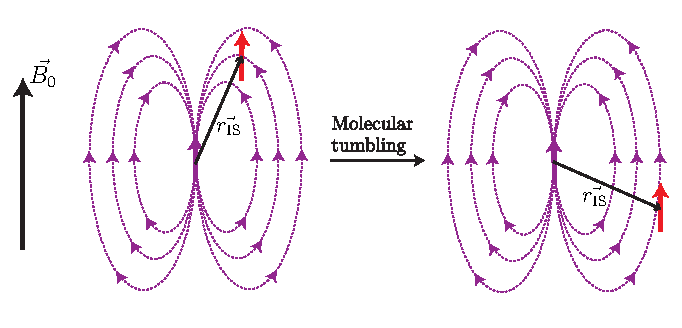
\includegraphics[scale=0.9]{./Figures/SimonsFigs/Dipolar.pdf}
\caption{An illustration of the dipolar interaction between two spins. Each dipole experiences the magnetic field emanating from the other dipole. The instantaneous magnetic field that the red spin experiences from the purple spin changes with time, due to molecular motion. It is this fluctuation in the local magnetic field that induces relaxation. Note that in this case, the two spins are assumed to be separated by a constant distance, as a result of chemical bonding.}
\label{Dipolar}
\end{figure}
The dipolar interaction is the direct interaction between two magnetic dipoles, as a result of one of the dipoles experiencing the magnetic field emanating from the other dipole, and vice-versa. The interaction is time-averaged to zero in solution, as the interaction is modulated by molecular diffusion. Despite this, the instantaneous dipolar interaction that two spins experience at any given time is one of the key mechanisms that induces relaxation in NMR. This principle is illustrated in Figure \ref{Dipolar}.\\
The anisotropy constant, $A_{\text{aniso}}^{\text{dipolar}} = d_{\text{IS}}$, is given by:
\begin{equation}
\label{DipConst}
d_{\text{IS}} = \left(\frac{\mu_0}{4 \pi}\right) \frac{\gamma_{\text{I}} \gamma_{\text{S}} \hbar}{r_{\text{IS}}^3}
\end{equation}
where $\gamma_{\text{I}}$ and $\gamma_{\text{S}}$ are the \textit{gyromagnetic ratios} of the two spins, and $r_{\text{IS}}$ is the distance that separates them. Note that the dipolar interaction does not feature an asymmetric component.
\subsubsection{The Chemical Shift Interaction}
The chemical shift interaction describes the generation of secondary magnetic fields about nuclear spins as a result of the motion of electrons induced by the external magnetic field, $\vec{B_0}$. This interaction, whilst also having an isotropic component, which directly impacts the position of peaks in spectra, often possesses both anisotropic and asymmetric components. This is a result of an uneven distribution electron density about a nucleus. However, it will be assumed that the chemical shift tensor is axially symmetrical, which is a treatment commonly adopted. The constant $A_{\text{aniso}}^{\text{CS}} = c_{\text{I}}$ is given by:
\begin{equation}
\label{CSAConst}
c_{\text{I}} = \gamma_{\text{I}} B_0 \Delta \sigma_{\text{I}}
\end{equation}
where $B_0$ is the magnetic field strength and $\Delta \sigma_{\text{I}}$, the anisotropy of the tensor, is given by $A_{33} - A_{11}$.
\section{Relaxation Models} \label{RelaxModels}
\subsection{Spherical Isotropic Motion} \label{SphericalSuperoperator}
The relaxation superoperator, $\hat{\hat{\Gamma}}$, is defined in \ref{superoperator}. The time-dependent Hamiltonian, $\hat{H}_1 (t)$, is simply a sum of all individual Hamiltonians that describe the relaxation mechanisms present in the spin-system of interest. For the case where the Hamiltonians may be simply described by one type of global motion, $\hat{H}_1 (t)$ adopts the form:
\begin{equation}
\begin{split}
\hat{H}_1 (t) &= \sum \limits_{i} \hat{H}_{\text{aniso}}^i (t)\\
&= \sqrt{6} \sum \limits_{i} A_{\text{aniso}}^i \sum \limits_{m = -2}^2 \sum \limits_{k = -2}^2 \mathfrak{D}_{m,k}^{(2)}(t) \mathfrak{D}_{k,0}^{(2)} (\Omega_i) \sum \limits_{n} \hat{T}_{i,k,n}^{(2)}
\end{split}
\end{equation}
where the expression spans all $i$ interactions considered. As a result, the relaxation superoperator can be written in the following form:
\begin{equation}
\begin{split}
\hat{\hat{\Gamma}} = &6 \sum \limits_{i_1, i_2} A_{\text{aniso}}^{i_1} A_{\text{aniso}}^{i_{2}} \sum \limits_{m_{1} = -2}^2 \sum \limits_{m_2 = -2}^2 \sum \limits_{k_1 = -2}^2 \sum \limits_{k_2 = -2}^2 \sum \limits_{n_1, n_2} \int \limits_0^{\infty} \overline{\mathfrak{D}_{m_1,k_1}^{(2)*}(t) \mathfrak{D}_{k_1,0}^{(2)*} (\Omega_{i_1})} \\
& \overline{\mathfrak{D}_{m_2,k_2}^{(2)}(t - \tau) \mathfrak{D}_{k_2,0}^{(2)} (\Omega_{i_2})} \comm{\hat{T}_{i_1, k_1, n_1}^{(2) \dagger}}{\comm{e^{-i \hat{H}_0 \tau}\hat{T}_{i_2, k_2, n_2}^{(2)} e^{i \hat{H}_0 \tau}}{}} d \tau
\end{split}
\end{equation}
Moving all time-independent terms outside of the integral, an acting the exponential operators on the operator $\hat{T}_{i_2, k_2, n_2}^{(2)}$ results in:
\begin{equation}
\begin{split}
\hat{\hat{\Gamma}} = &6 \sum \limits_{i_1, i_2} A_{\text{aniso}}^{i_1} A_{\text{aniso}}^{i_{2}} \sum \limits_{m_{1} = -2}^2 \sum \limits_{m_2 = -2}^2 \sum \limits_{k_1 = -2}^2 \sum \limits_{k_2 = -2}^2 \mathfrak{D}_{k_1,0}^{(2)*} (\Omega_{i_1}) \mathfrak{D}_{k_2,0}^{(2)} (\Omega_{i_2}) \sum \limits_{n_1, n_2} \\
& \comm{\hat{T}_{i_1, k_1, n_1}^{(2) \dagger}}{\comm{\hat{T}_{i_2, k_2, n_2}^{(2)}}{}} \int \limits_0^{\infty} \overline{\mathfrak{D}_{m_1,k_1}^{(2)*}(t) \mathfrak{D}_{m_2,k_2}^{(2)}(t - \tau)} e^{-i \omega_{k_2, n_2} \tau} d \tau
\end{split}
\end{equation}
This expression can be simplified by noting that the \textit{correlation function}, for the case of spherical isotropic rotation, is given by\cite{RN40}:
\begin{equation}\\
\label{CorrFuncSpher}
\overline{\mathfrak{D}_{m_1,k_1}^{(2)*}(t) \mathfrak{D}_{m_2,k_2}^{(2)} (t - \tau)} = \frac{\delta_{m_1,m_2} \delta_{k_1,k_2}}{5} e^{-\frac{\tau}{\tau_{\text{c}}}}
\end{equation}
where $\tau_{\text{c}}$ is the \textit{rotational correlation time}. In an isotropic solution, $\tau_{\text{c}}$ is roughly the rotational correlation time of the molecule, defined as the average time taken for the molecule to be deflected by 1 radian\cite{RN2}. The Kronecker Delta functions, $\delta_{m_1,m_2}$ and $\delta_{k_1,k_2}$ indicate that only terms for which $m_1 = m_2 = m$ and $k_1 = k_2 = k$ will be non-zero, such that:
\begin{equation}
\label{SupOpSpher}
\begin{split}
\hat{\hat{\Gamma}} = &\frac{6}{5} \sum \limits_{i_1, i_2} A_{\text{aniso}}^{i_1} A_{\text{aniso}}^{i_{2}} \sum \limits_{m = -2}^2 \sum \limits_{k = -2}^2 \sum \limits_{n_1, n_2} \mathfrak{D}_{k,0}^{(2)*} (\Omega_{i_1}) \mathfrak{D}_{k,0}^{(2)} (\Omega_{i_2})\\
& \comm{\hat{T}_{i_1, k, n_1}^{(2) \dagger}}{\comm{\hat{T}_{i_2, k, n_2}^{(2)}}{}} \int \limits_0^{\infty} e^{-\frac{\tau}{\tau_{\text{c}}}} e^{-i \omega_{k, n_2} \tau} d \tau
\end{split}
\end{equation}
The real part of the integral on the right hand side of \ref{SupOpSpher} is called the \textit{spectral density function}, $J(\tau_{\text{c}}, \omega_{k,n_2})$, which takes the form:
\begin{equation}
\label{SpecDenSpher}
J(\tau_{\text{c}}, \omega_{k,n_2}) = \text{Re} \left[\int \limits_0^{\infty} e^{-\frac{\tau}{\tau_{\text{c}}}} e^{-i \omega_{k, n_2} \tau} d \tau \right]= \frac{\tau_{\text{c}}}{1 + \omega_{k,n_2}^2 \tau_{\text{c}}^2}
\end{equation}
The imaginary component can be incorporated into $\hat{H}_0$, and thus has no impact on relaxation\cite{RN2}. 
Note that there are no longer any components in this expression that are dependent of $m$, so the summation over this index is redundant. A final expression for the rate of relaxation of density matrix element $\hat{\rho}_{rs}$ is given by:
\begin{equation}
\begin{split}
\label{SpherOpElement}
\Gamma_{rs} =&\frac{6}{5} \sum \limits_{i_1, i_2} A_{\text{aniso}}^{i_1} A_{\text{aniso}}^{i_2} \sum \limits_{k = -2}^2 \mathfrak{D}_{k,0}^{(2)*} (\Omega_{i_1}) \mathfrak{D}_{k,0}^{(2)} (\Omega_{i_2})\\
&\sum \limits_{n_1, n_2} \frac{\bra{\hat{\rho}_s} \ket{\comm{\hat{T}_{i_1, k, n_1}^{(2) \dagger}}{\comm{\hat{T}_{i_2,k,n_2}^{(2)}}{\hat{\rho}_r}}}}{\sqrt{\bra{\hat{\rho}_r} \ket{\hat{\rho}_r} \bra{\hat{\rho}_s} \ket{\hat{\rho}_s}}} J(\tau_{\text{c}}, \omega_{k,n_2})
\end{split}
\end{equation}
I illustrate a rigorous calculation of certain relaxation rates in an IS spin system using this model in Appendix B.
\subsection{Methyl Rotation}\label{MethylRot}
Using the definition of $\hat{H}_1 (t)$ in \ref{MethylHam}, and applying similar adjustments to those presented in Section \ref{SphericalSuperoperator}, the relaxation superoperator takes the following form:
\begin{equation}
\begin{split}
\hat{\hat{\Gamma}} = &6 \sum \limits_{i_1, i_2} A_{\text{aniso}}^{i_1} A_{\text{aniso}}^{i_{2}} \sum \limits_{m_{1} = -2}^2 \sum \limits_{m_2 = -2}^2 \sum \limits_{k_1 = -2}^2 \sum \limits_{k_2 = -2}^2 \sum \limits_{n_1, n_2} \mathfrak{D}_{k_1,0}^{(2)*} (\Omega_{i_1}) \mathfrak{D}_{k_2,0}^{(2)} (\Omega_{i_2}) \\
& \comm{\hat{T}_{i_1, k_1, n_1}^{(2) \dagger}}{\comm{\hat{T}_{i_2, k_2, n_2}^{(2)}}{}} \int \limits_0^{\infty} \overline{\mathfrak{D}_{m_1,k_1}^{(2) \text{c} *}(t) \mathfrak{D}_{k_1,k_1}^{(2) \text{m} *}(t) \mathfrak{D}_{m_2,k_2}^{(2) \text{c}}(t - \tau) \mathfrak{D}_{k_2,k_2}^{(2) \text{m}}(t - \tau)} e^{-i \omega_{k_2,n_2} \tau} d \tau
\end{split}
\end{equation}
Assuming the motion of the methyl group, and the global tumbling are independent, the 4-term correlation function can be split into two separate correlation functions. The first of these, in analogous fashion to \ref{CorrFuncSpher}, is given by:
\begin{equation}
\overline{\mathfrak{D}_{m_1,k_1}^{(2) \text{c}*}(t) \mathfrak{D}_{m_2,k_2}^{(2) \text{c}} (t - \tau)} = \frac{\delta_{m_1,m_2} \delta_{k_1,k_2}}{5} e^{-\frac{\tau}{\tau_{\text{c}}}}
\end{equation}
The second of these, involving the Wigner D-elements corresponding to rotation about the methyl axis, differ depending on the motional model that is adopted. Two models are considered:
\begin{enumerate}
\item The I-spins rapidly interchange by undergoing jumps between three different permitted sites. Such a model is often referred to as the \textit{Woessner Model}\cite{RN32}.
\item The I-spins are able to undergo random rotational diffusion, whilst maintaining a fixed orientation relative to each other. This will be referred to as the \textit{Diffusive Model}.
\end{enumerate}
Illustrations of these models are presented in Figure \ref{WoessnerDiffusive}.
\begin{figure}
\centering
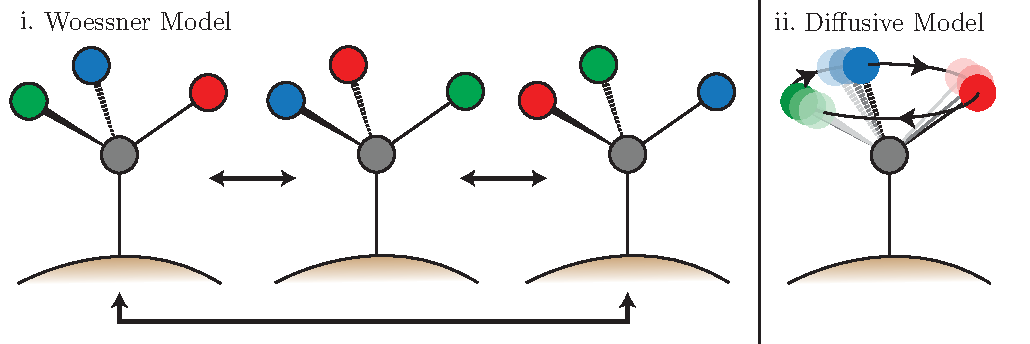
\includegraphics[scale=0.8]{./Figures/SimonsFigs/WoessnerDiffusion.pdf}
\caption{Illustrations of the two types of methyl motion considered in this thesis. i. In the Woessner Model, the three I-spins rapidly exchange between three fixed sites. ii. In the Diffusive Model, the three I-spins are able to rotate freely about a ring, whilst maintaining a their relative orientations to each other.}
\label{WoessnerDiffusive}
\end{figure}
The correlation function adopts the following form\cite{RN4}:
\begin{equation}
\overline{\mathfrak{D}_{k_1,k_1}^{(2) \text{m}*}(t) \mathfrak{D}_{k_2,k_2}^{(2) \text{m}} (t - \tau)} = \delta_{k_1,k_2} e^{-\frac{k_{\text{DW}}^2 \tau}{\tau_{\text{m}}}}
\end{equation}
The constant $k_{\text{DW}}$ adopts different values depending on the model adopted, which are given in Table \ref{kDW}.
\begin{table}[]
\centering
\begin{tabular}{l|l|l}
$k$     & $k_{\text{DW}}$, Woessner & $k_{\text{DW}}$, Diffusive \\ \hline
$0$     & $0$                       & $0$                        \\
$\pm 1$ & $\pm 1$                   & $\pm 1$                    \\
$\pm 2$ & $\pm 1$                   & $\pm 2$                   
\end{tabular}
\caption{The values adopted by the constant, $k_{\text{DW}}$, which is dependent of the value of $k$, and the methyl rotation model considered.}
\label{kDW}
\end{table}
Accounting for these identities, the expression for $\hat{\hat{\Gamma}}$ collapses to:
\begin{equation}
\begin{split}
\hat{\hat{\Gamma}} = &\frac{6}{5} \sum \limits_{i_1, i_2} A_{\text{aniso}}^{i_1} A_{\text{aniso}}^{i_{2}} \sum \limits_{k = -2}^2 \sum \limits_{n_1, n_2} \mathfrak{D}_{k,0}^{(2)*} (\Omega_{i_1}) \mathfrak{D}_{k,0}^{(2)} (\Omega_{i_2}) \\
&\comm{\hat{T}_{i_1, k, n_1}^{(2) \dagger}}{\comm{\hat{T}_{i_2, k, n_2}^{(2)}}{}}\int \limits_0^{\infty} e^{-\frac{\tau}{\tau_{\text{c}}}} e^{-\frac{k_{\text{DW}}^2 \tau}{\tau_{\text{m}}}} e^{-i \omega_{k, n_2} \tau} d \tau \\
= &\frac{6}{5} \sum \limits_{i_1, i_2} A_{\text{aniso}}^{i_1} A_{\text{aniso}}^{i_{2}} \sum \limits_{k = -2}^2 \mathfrak{D}_{k,0}^{(2)*} (\Omega_{i_1}) \mathfrak{D}_{k,0}^{(2)} (\Omega_{i_2}) \\
&\sum \limits_{n_1, n_2} \comm{\hat{T}_{i_1, k, n_1}^{(2) \dagger}}{\comm{\hat{T}_{i_2, k, n_2}^{(2)}}{}} J\left(\frac{\tau_{\text{c}} \tau_{\text{m}}}{\tau_{\text{m}} + \tau_{\text{c}} k_{\text{DW}}^2}, \omega_{k,n_2}\right)
\end{split}
\end{equation}
where $J\left(\frac{\tau_{\text{c}} \tau_{\text{m}}}{\tau_{\text{m}} + \tau_{\text{c}} k_{\text{DW}}^2}, \omega_{k,n_2}\right)$, the spectral density function for this model, is given by:
\begin{equation}
\label{SpecDenMeth}
J\left(\frac{\tau_{\text{c}} \tau_{\text{m}}}{\tau_{\text{m}} + \tau_{\text{c}} k_{\text{DW}}^2}, \omega_{k,n_2}\right) = \frac{\frac{\tau_{\text{c}} \tau_{\text{m}}}{\tau_{\text{m}} + \tau_{\text{c}} k_{\text{DW}}^2}}{1 + \left(\frac{\tau_{\text{c}} \tau_{\text{m}}}{\tau_{\text{m}} + \tau_{\text{c}} k_{\text{DW}}^2}\right)^2 \omega_{k,n_2}^2}
\end{equation}
With the theory established, the attention now moves to comparing the relaxation models outlined in this chapter, along with models already presented in the literature. The next chapter outlines some theoretical relaxation rate calculations on I$_3$S spin systems that have been conducted in an attempt to achieve this. After this, some calculations comparing relaxation in $^{13}$CH$_3$ and $^{13}$CF$_3$ moieties are used to predict the viability of a trifluoromethyl moiety as an effective TROSY probe.
% Report-TheoreticalCalculations.tex
% Simon Hulse
% simonhulse@protonmail.com
% Last Edited: Wed 27 Nov 2024 02:54:44 PM EST

% !TeX root = ./Report-Body.tex
\allowdisplaybreaks
\chapter{Theoretical Calculations}
The simulate NMR experiments, it will be necessary to determine the relaxation rates of all coherences that exist. For an I$_3$S spin system, this requires determining all the matrix elements, $\Gamma_{rs}$, of the $256 \times 256$ relaxation superoperator. These elements will give great insight into how well different NMR experiments will perform. As a step towards achieving this, a python programme was developed from code written within the Baldwin group, in order to implement the relaxation models presented in Section \ref{RelaxModels}. This script produces symbolic rate expressions as an output. For numerical considerations, a programme able to parse the symbolic outputs was created for this thesis. Explicit examples of calculations using these scripts are presented below. Highly detailed insights can be made about relaxation phenomena in I$_3$S spin-systems as a result.
\section{Relaxation Rates Considered} \label{RatesConsidered}
A selection of relaxation rate calculations utilising the models established are presented in the subsequent sections of this chapter. The rates chosen were those of S-spin single-quantum coherences. These coherences correspond to the product operators $\hat{S}^{\alpha \alpha \alpha +}$, $\hat{S}^{\alpha \alpha \beta +}$, $\hat{S}^{\alpha \beta \beta +}$, and $\hat{S}^{\beta \beta \beta +}$, whose rates are given by $\Gamma_{2,\text{C}}^{i}$, where $i \in \{\alpha \alpha \alpha, \alpha \alpha \beta, \alpha \beta \beta, \beta \beta \beta\}$. These are responsible for the observable signal in $^{13}$C NMR experiments, giving rise to a quartet peak structure, Figure \ref{CQuart}. Relaxation rates of these coherences can be determined rather easily experimentally, making it possible to assess the effectiveness of our relaxation models. Table \ref{Operators} provides explicit definitions of the relevant operators using the single-element basis. All relaxation rates considered are auto-relaxation rates, corresponding to diagonal elements of the relaxation super operator (i.e. $\Gamma_{r,r}$, where $r$ is one of the product operators listed in Table \ref{Operators}).
\begin{table}[]
\centering
\begin{tabular}{l|l}
Operator                           & Definition                                                                                                                                                                                                        \\ \hline
$\hat{S}^{\alpha \alpha \alpha +}$ & $\hat{I}_1^{\alpha} \hat{I}_2^{\alpha} \hat{I}_3^{\alpha} \hat{S}^{+}$                                                                                                                                            \\
$\hat{S}^{\alpha \alpha \beta +}$  & $\hat{I}_1^{\alpha} \hat{I}_2^{\alpha} \hat{I}_3^{\beta} \hat{S}^{+} + \hat{I}_1^{\alpha} \hat{I}_2^{\beta} \hat{I}_3^{\alpha} \hat{S}^{+} + \hat{I}_1^{\beta} \hat{I}_2^{\alpha} \hat{I}_3^{\alpha} \hat{S}^{+}$ \\
$\hat{S}^{\alpha \beta \beta +}$   & $\hat{I}_1^{\alpha} \hat{I}_2^{\beta} \hat{I}_3^{\beta} \hat{S}^{+} + \hat{I}_1^{\beta} \hat{I}_2^{\alpha} \hat{I}_3^{\beta} \hat{S}^{+} + \hat{I}_1^{\beta} \hat{I}_2^{\beta} \hat{I}_3^{\alpha} \hat{S}^{+}$    \\
$\hat{S}^{\beta \beta \beta +}$    & $\hat{I}_1^{\beta} \hat{I}_2^{\beta} \hat{I}_3^{\beta} \hat{S}^{+}$
\end{tabular}
\caption{Definitions of product operators which describe the S-spin single quantum coherences.}
\label{Operators}
\end{table}
\section{$^{13}$C Transverse Rates in a Methyl Moiety}
A significant amount of literature exists describing methyl relaxation rates, primarily due to the emergence of methyl-TROSY as a well established technique for studying high mass biomolecules. Expressions describing $^{13}$C transverse relaxation rates, $\Gamma_{2,\text{C}}^{i}$, have been presented previously in the literature, using different assumptions. A couple of these descriptions are now outlined, before we extend the treatment.
\begin{figure}
\centering
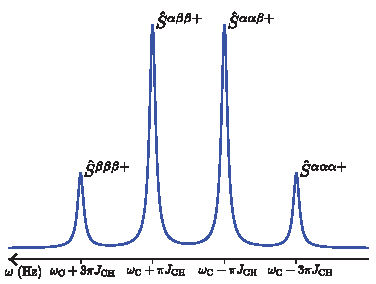
\includegraphics[scale=1.2]{./Figures/SimonsFigs/13CQuartet.pdf}
\caption{A simulated 1D $^{13}$C spectrum of a methyl moiety. A quartet of peaks are present, as a result of scalar coupling between the $^{13}$C nucleus and the $^{1}$H nuclei. The four peaks appear at frequencies $\omega_{\text{C}} - 3 \pi J_{\text{CH}}$, $\omega_{\text{C}} - \pi J_{\text{CH}}$, $\omega_{\text{C}} + \pi J_{\text{CH}}$, and $\omega_{\text{C}} + 3 \pi J_{\text{CH}}$, respectively, where $\omega_{\text{C}}$ is the resonance frequency of the $^{13}$C nucleus. Each peak is labelled by the product operator that corresponds to the signal it derives from.}
\label{CQuart}
\end{figure}
\subsection{Previous Accounts} \label{PreviousModels}
\subsubsection{Ollerenshaw et al., 2003}
In a paper illustrating the theoretical underpinning of methyl-TROSY, Ollerenshaw et al. presented remarkably simple expressions of the rates \cite{RN17}. Only dipolar interactions were considered. The methyl moiety's rotational motional motion about its C$_3$ axis was assumed to be infinitely fast. On top of what is presented in Section \ref{MethylRot}, an additional type of motion was included - that of the methyl symmetry axis. In Chapter 2, the motion of the symmetry axis is assumed to be perfectly correlated with the rest of the molecule. The possibility of this not being the case is approximated by a model-free approach, first described by Lipari and Szabo\cite{RN31}. Moreover, the macromolecular limit was invoked, in which it is assumed that $\omega_{\text{S}} \tau_{\text{c}} \gg 1$, where $\omega_{\text{S}}$ corresponds to the $^{13}$C Larmor frequency. In this limit, all spectral density terms for which $\omega \neq 0$ are negligibly small, and thus do not contribute to the rate expression. A term accounting for dipolar interactions with external protons was also included. NMR spectra are conventionally run on samples with high levels of deuteration in order to reduce such external interactions\footnote{Incorporation of deuterium into the sample reduces external dipolar interactions, on account of the smaller gyromagnetic ratio of deuterium, relative to proton ($\gamma_{\text{H}} \approx 6 \gamma_{\text{D}}$)}. Labelling strategies specific to the methyl-TROSY technique have been developed with this intention\cite{RN45}. Despite this, external dipolar interactions can still a have marked impact on relaxation rates, such that a full-scale calculation should include them.
\subsubsection{Hansen et al., 2009}
Less drastic approximations were presented by Hansen et al.\cite{RN4} As well as dipolar interactions, the CSA of the $^{13}$C nucleus was included as a mechanism able to induce relaxation. The Woessner Model, described in Chapter 2, was invoked to describe methyl rotation. Spectral density terms, $J\left(\tau_{\text{c}}, \omega\right)$\footnote{These spectral densities arise when $k_{\text{DW}} = 0$} with $\omega = \omega_{\text{S}}$ were included along as those with $\omega = 0$. It was again assumed that methyl rotation is rapid relative to the global motion of the molecule, meaning  $\tau_{\text{c}} \gg \tau_{\text{m}}$. In this limit, spectral density terms, $J\left(\frac{\tau_{\text{c}} \tau_{\text{m}}}{\tau_{\text{m}} + \tau_{\text{c}} k_{\text{DW}}^2}, \omega_{k,n_2}\right)$, for which $k_{\text{DW}} \neq 0$, reduce to $\frac{\tau_{\text{m}}}{k_{\text{DW}}^2} = \tau_{\text{m}}$.\\
To account for external interactions from remote protons, an additional term, $\frac{3}{2} \Gamma_{\text{sel}}$, was included, where $\Gamma_{\text{sel}} = \Gamma_{1,\text{H}}^{zz} - \Gamma_{1,\text{H}}^{z}$. $\Gamma_{1,\text{H}}^{z}$ and $\Gamma_{1,\text{H}}^{zz}$ are the auto-relaxation rates of the operators $2\hat{I}_z\hat{S}_z$ and $4\hat{I}_z\hat{I}_z\hat{S}_z$ respectively\footnote{$2\hat{I}_z\hat{S}_z = 2\hat{I}_{1z}\hat{S}_z + 2\hat{I}_{2z}\hat{S}_z + 2\hat{I}_{3z}\hat{S}_z$, and $4\hat{I}_z\hat{I}_z\hat{S}_z = 4\hat{I}_{1z}\hat{I}_{2z}\hat{S}_z+ 4\hat{I}_{1z}\hat{I}_{3z}\hat{S}_z + 4\hat{I}_{2z}\hat{I}_{3z}\hat{S}_z$}. This term stems from methyl proton longitudinal relaxation, driven by dipolar couplings with external protons. Such interactions are able to 'flip' the spin state of the external protons, and leads to an additional source of relaxation in the methyl moiety. Explicit expressions of $\Gamma_{1,\text{H}}^{z}$ and $\Gamma_{1,\text{H}}^{zz}$ were not presented by Hansen et al., though $\Gamma_{1,\text{H}}^{zz} - \Gamma_{1,\text{H}}^{z}$ was said to scale with $J(\tau_{\text{c}},0)$ in the macromolecular limit.  The desired term was obtained by using our result, and invoking the macromolecular limit.
\subsection{Comparison of the Models}
The accounts in Section \ref{PreviousModels} were compared with the spherical isotropic, Woessner and diffusive models presented in Chapter 2. This was done by assuming a $^{13}$C$^{1}$H$_{3}$ moiety, with a perfect tetrahedral geometry, such that the angle $\beta$ between the threefold rotation axis and the C-H bond vectors is $\cos^{-1}(-\frac{1}{3}) \approx \ang{109.47}$. Dipolar interactions with spins external to the methyl group were accounted for by assuming a single external proton was present, at an average distance of $\num{3} \si{\angstrom}$ from the methyl protons. The other parameters of relevance are stated in the caption of Figure \ref{CH3Models}. Explicit expressions derived from all relaxation models are presented in Appendix C. The angles of rotations applied to each tensor, to bring them into the molecular frame, are given in Table \ref{tab3.1}.\\
\begin{table}[]
\centering
\begin{tabular}{l|l}
Interaction tensor & $(\alpha, \beta)$           \\ \hline
$d_{\text{IS}} (1)$                              & $(\ang{0}, \ang{109.47})$   \\
$d_{\text{IS}} (2)$                              & $(\ang{120}, \ang{109.47})$ \\
$d_{\text{IS}} (3)$                              & $(\ang{240}, \ang{109.47})$ \\
$d_{\text{II}} (1)$                              & $(\ang{90}, \ang{270})$     \\
$d_{\text{II}} (2)$                              & $(\ang{90}, \ang{210})$     \\
$d_{\text{II}} (3)$                              & $(\ang{90}, \ang{150})$     \\
$c_{\text{S}}$                                   & $(\ang{0}, \ang{0})$        \\
$c_{\text{I}} (1)$                               & $(\ang{0}, \ang{109.47})$   \\
$c_{\text{I}} (2)$                               & $(\ang{120}, \ang{109.47})$ \\
$c_{\text{I}} (3)$                               & $(\ang{240}, \ang{109.47})$
\end{tabular}
\caption{The angles characterising the rotations of all interaction tensors into the Molecular frame.}
\label{tab3.1}
\end{table}
\begin{figure}
\centering
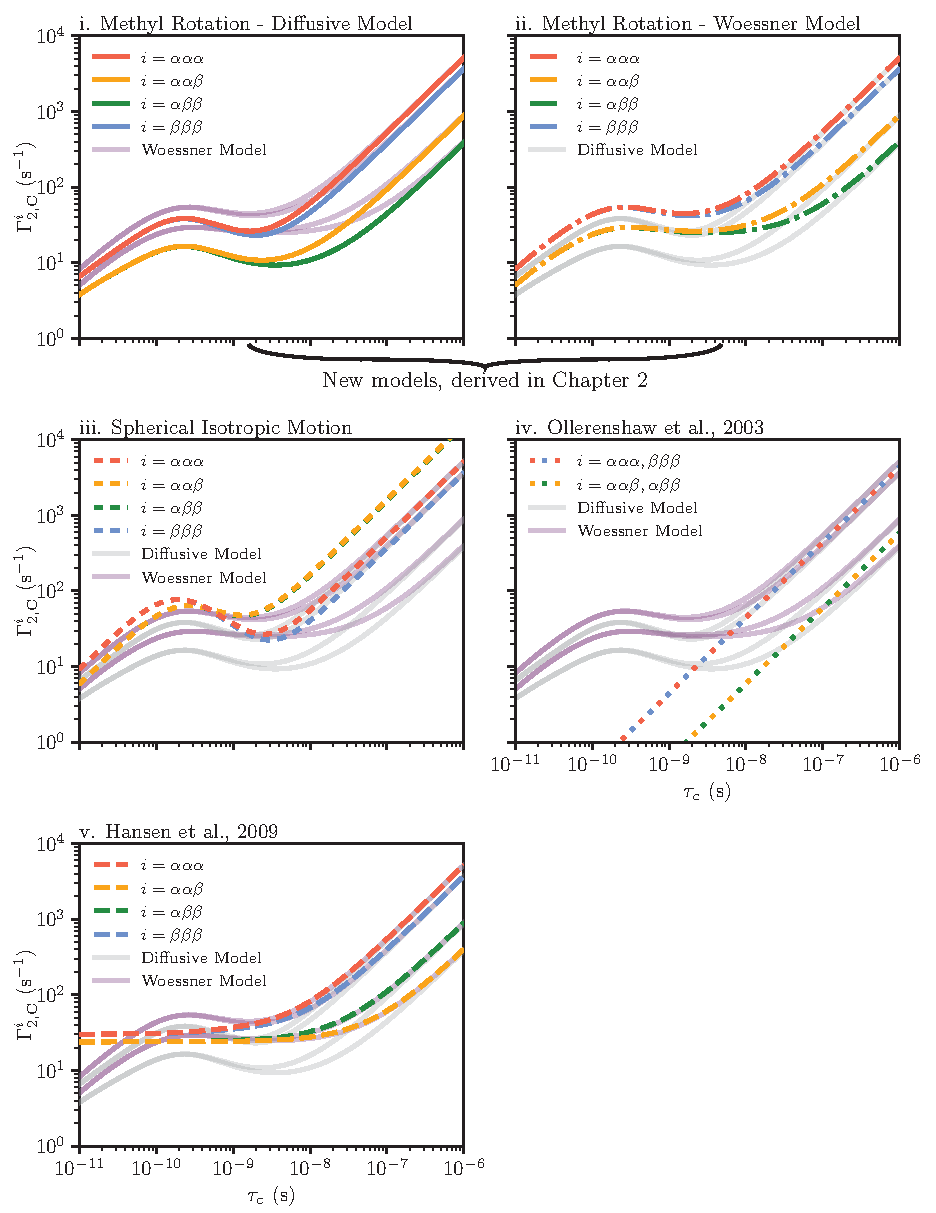
\includegraphics[scale=1]{./Figures/SimonsFigs/CH3models.pdf}
\caption{%
Plots of relaxation rate versus global tumbling correlation time,
$\tau_{\text{c}}$, for various I$_3$S relaxation models.
Parameters used: $B_0 = \num{14.1} \si{\tesla}$,
corresponding to a $\num{600} \si{\mega\myhertz}$ spectrometer,
$\gamma_{\text{S}} = \num{67.283e6} \si{\radian\per\second\per\tesla}$,
$\gamma_{\text{I}} = \num{267.513e6} \si{\radian\per\second\per\tesla}$,
$r_{\text{IS}} = r_{\text{II}} = \num{1.09} \si{\angstrom}$,
$\theta = \ang{109.47}$,
$\tau_{\text{m}} = \num{50} \si{\pico\second}$,
$\Delta \sigma_{\text{S}} = 20 \text{ppm}$,
$\Delta \sigma_{\text{I}} = 1 \text{ppm}$,
$S_{\text{axis}} = 1$ (this is described in Appendix D).
All plots have the results of the diffusive and Woessner model calculations
superimposed, for easy comparison.
}
\label{CH3Models}
\end{figure}
In Figure \ref{CH3Models}, plots ii., and v. show very good agreement for large values of $\tau_{\text{c}}$. This is exactly what is expected, since the both sets of expressions for the rates were derived using the Woessner model, but Hansen et al. apply the macromolecular limit. There are relatively marked differences in behaviour between the Woessner model (plot ii.) and the diffusive model (plot i.) when considering more rapid tumbling (smaller $\tau_{\text{c}}$ values). The trend for a decrease in rates with increasing $\tau_{\text{c}}$ in the region of $\tau_{\text{c}} \approx \num{e-9} \si{\second}$ is not something that was anticipated, and its origin is discussed below. The result of Ollerenshaw et al. resembles plots i., ii., and v. somewhat in the macromolecular limit. However, inclusion of the $^{13}$C CSA causes the rates of the other methyl rotation models to deviate from this model. The plots suggest that the carbon CSA has a noticeable, but non-dominating impact on the rates in the macromolecular limit.\\
It is clear that the spherical isotropic model in iii. is inappropriate, primarily as there is a gross overestimation of the inner line ($\alpha \alpha \beta$ and $\alpha \beta \beta$) relaxation rates, relative to the models that incorporate methyl rotation.
\subsection{Investigating Individual Contributions to the Rates}
The complete set of rate expressions derived are given in Appendix D, however in order to gain a more in-depth understanding of the form of the plots in Figure \ref{CH3Models}, rate of one specific line in the quartet: $\alpha \alpha \alpha$ (red) was considered in detail. Despite the very large number of terms that feature in the rate expressions, only a few terms tend to contribute significantly with any given value of $\tau_{\text{c}}$, and some always have a negligible impact. Over the entire range of $\tau_{\text{c}}$ considered in Figure \ref{CH3Models}, a very good approximation of $\Gamma_{2,\text{C}}^{\alpha\alpha\alpha}$, using the Diffusive and Woessner Models is given by the expression:
\begin{equation}
\label{eq3.3}
\begin{split}
\Gamma_{2,\text{C}}^{\alpha\alpha\alpha} \approx &\frac{1}{5} d_{\text{IS}}^2 J(\tau_{\text{c}},0) + \frac{4}{15} d_{\text{IS}}c_{\text{S}} J\left(\tau_{\text{c}},0\right)+ \frac{4}{45} c_{\text{S}}^2 J\left(\tau_{\text{c}},0\right) \\ &+ \frac{3}{20} d_{\text{IS}}^2  J(\tau_{\text{c}}, \omega_{\text{C}}) +
d_{\text{II}}^2\bigg[\frac{27}{80}J\left(\frac{\tau_{\text{c}}\tau_{\text{m}}}{\tau_{\text{m}}+k_{\text{DW}}^2\tau_{\text{c}}},\omega_{\text{I}}\right)+\frac{9}{20}J\left(\tau_{\text{c}},\omega_{\text{I}}\right)\\
& +\frac{27}{20}J\left(\frac{\tau_{\text{c}}\tau_{\text{m}}}{\tau_{\text{m}}+k_{\text{DW}}^2\tau_{\text{c}}},2\omega_{\text{I}}\right)+\frac{9}{20}J\left(\tau_{\text{c}},2\omega_{\text{I}}\right)\bigg] + \Gamma_{\text{ext}}
\end{split}
\end{equation}
where $k_{\text{DW}} = 1\ (2)$ in the case of the Woessner (diffusive) model. $\Gamma_{\text{ext}}$ contains all contributions due to dipolar interactions with external nuclei. This is given by:
\begin{equation}
\label{External}
\Gamma_{\text{ext}} = \frac{3}{20}\left[J(\tau_{\text{c}},0) + 3J(\tau_{\text{c}},\omega_{\text{I}}) + 6J(\tau_{\text{c}},2 \omega_{\text{I}}) \right] \sum \limits_i d_{\text{II},i}^2
\end{equation}
where the summation spans all the $i$ external nuclei considered, and $d_{\text{II},i}$ is given by:
\begin{equation}
d_{\text{II},i} = \left( \frac{\mu_0}{4 \pi}\right) \frac{\gamma_{\text{I}}^2 \hbar}{r_{\text{II},i}^3}
\end{equation}
$r_{\text{II},i}$ is the average distance separating external proton $i$ from the methyl protons.\\
Plots i. and ii. in Figure \ref{IndividualTerms} show the variation of $\Gamma_{2,\text{S}}^{\alpha\alpha\alpha}$ with $\tau_{\text{c}}$, using the both Woessner and diffusive models. Also, the individual contributions stated in \ref{eq3.3} are plotted.  Note that external contributions have been neglected in these plots. It can be seen that terms arising from $^{1}$H-$^{1}$H dipolar interactions dominate when faster tumbling is considered (i.e. on the left-hand side of the plots). This is the case for two reasons: (a) the constant $d_{\text{II}}^2 = \frac{\mu_0^2 \gamma_{\text{I}}^4 \hbar^2}{16 \pi^2 r_{\text{II}}^6}$ is large, owing to the large gyromagnetic ratio of $^1$H. (b) the spectral density terms $J\left(\tau_{\text{c}},\omega_{\text{I}}\right)$ and $J\left(\tau_{\text{c}},2\omega_{\text{I}}\right)$ are of significant magnitude for small $\tau_{\text{c}}$ values, having maxima at $\tau_{\text{c}} = \num{1.67e-9} \si{\second}$ and $\tau_{\text{c}} = \num{8.33e-10} \si{\second}$, respectively\footnote{These maxima occur when $\dv{J\left(\tau_{\text{c}},\omega\right)}{\tau_{\text{c}}} = 0$, which corresponds to $\tau_{\text{c}} = |\frac{1}{\omega}|$.}. Contributions containing spectral densities that possess smaller frequencies (i.e. $0$, $\omega_{\text{S}}$ etc.) are comparatively negligible at these $\tau_{\text{c}}$ values. It is these terms that are the major source of deviation between plots ii. and v. in Figure \ref{CH3Models}. Whilst the Woessner model is employed in both cases, spectral density terms, $J\left(\tau_{\text{c}}, \omega \right)$, involving frequencies $\omega_{\text{I}}$ and $2 \omega_{\text{I}}$ are neglected by Hansen et al.\\
\begin{figure}
\centering
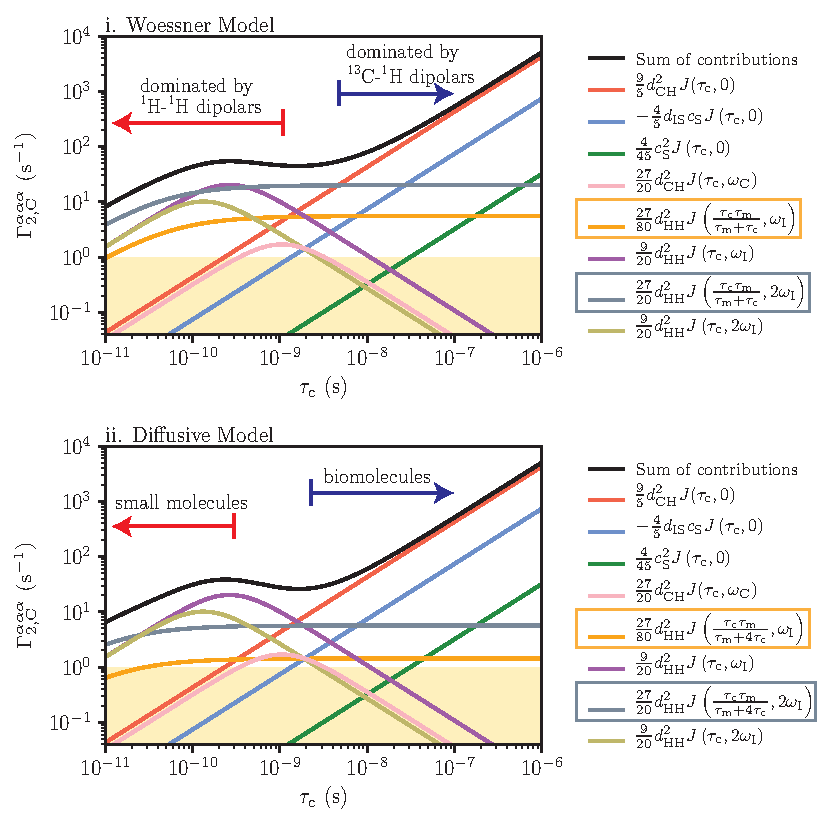
\includegraphics[scale=1]{./Figures/SimonsFigs/Contributions.pdf}
\caption{Plots of relaxation rate versus global tumbling correlation time, $\tau_{\text{c}}$, for the $\alpha \alpha \alpha$ peak in the $^{13}$C quartet (black lines), using the Woessner model (i.) and diffusive model (ii.). Individual terms in the rate expressions that contribute significantly over any range of $\tau_{\text{c}}$ are also plotted (coloured lines). All other terms reside within the yellow shaded region (or below the scale) for all $\tau_{\text{c}}$ values, and do not contribute to the rate in a significant manner in any region of the plot. The terms that cause differences between the two models are highlighted.}
\label{IndividualTerms}
\end{figure}
It is also in this region of the plot where the Diffusive and Woesssner models show the greatest deviations from each other. The lower rates predicted by the diffusive model are a result of the terms corresponding to the grey and orange lines in Figure \ref{IndividualTerms}. These terms are of a smaller magnitude when the diffusive model is considered, as they have spectral densities with $k_{\text{DW}} = 2$ associated with them. With the Woessner model, these terms have $k_{\text{DW}} = 1$ instead.\\
When larger values of $\tau_{\text{c}}$ are considered, the relaxation rates enter a linear regime, which corresponds to the macromolecular limit. This is since terms with spectral densities possessing frequency $0$ become dominant:
\begin{equation}
J(\tau_{\text{c}}, 0) = \tau_{\text{c}}
\end{equation}
For both the Diffusive and Woessner Models, the expressions for all four rates
collapse as follows, when only $J(\tau_{\text{c}}, 0)$ terms are considered:
\begin{equation}\label{MacroLim}
\begin{gathered}
\Gamma_{2,S}^{\alpha\alpha\alpha} \approx \frac{\tau_{\text{c}}}{45} \left( 9 d_{\text{IS}}^2  + 12 d_{\text{IS}} c_{\text{S}} + 4 c_{\text{S}}^2 \right) + \frac{3 \tau_{\text{c}} }{20} \sum \limits_i d_{\text{II},i}^2\\
\Gamma_{2,S}^{\alpha\alpha\beta} \approx \frac{\tau_{\text{c}}}{45} \left(d_{\text{IS}}^2  + 4 d_{\text{IS}} c_{\text{S}} + 4 c_{\text{S}}^2 \right) + \frac{3 \tau_{\text{c}}}{20} \sum \limits_i d_{\text{II},i}^2 \\
\Gamma_{2,S}^{\alpha\beta\beta} \approx \frac{\tau_{\text{c}}}{45} \left(d_{\text{IS}}^2  - 4 d_{\text{IS}} c_{\text{S}} + 4 c_{\text{S}}^2 \right) + \frac{3 \tau_{\text{c}} }{20} \sum \limits_i d_{\text{II},i}^2 \\
\Gamma_{2,S}^{\beta\beta\beta} \approx \frac{\tau_{\text{c}}}{45} \left(9 d_{\text{IS}}^2  - 12 d_{\text{IS}} c_{\text{S}} + 4 c_{\text{S}}^2 \right) + \frac{3 \tau_{\text{c}}}{20} \sum \limits_i d_{\text{II},i}^2
\end{gathered}
\end{equation}
From Figure \ref{IndividualTerms}, it is clear that the first term in these expressions, proportional to $d_{\text{IS}}^2$, is dominant in this limit, though $^{13}$C CSA contributions do also contribute to a noticeable extent.
\subsection{Summarising the Results}
The rate expressions presented by Ollerenshaw et al. are impressively accurate for methyl groups in molecules with large $\tau_{\text{c}}$ values, despite their simplicity relative to other models considered. This boils down to the fact that one particular term, arising from $^{13}$C-$^1$H dipolar interactions, dominates the relaxation behaviour in the macromolecular limit. Using fewer approximations, and crucially incorporating $^{13}$C CSA contributions, the model presented by Hansen et al. is highly accurate in the macromolecular limit. Their model and has been implemented in relaxation studies of methyls in proteins\cite{RN4}, indicating its validity. However, this model would be inadequate for calculations involving $^{13}$CF$_3$ moieties, since no consideration of the I-spin CSA is made. Whilst justifiable for methyl groups, where $\Delta \sigma_{\text{H}}$ is typically negligibly small, only models which include I-spin CSAs are likely to be appropriate for $^{13}$CF$_3$ studies.
\section{Comparing $^{13}$CH$_3$ with $^{13}$CF$_3$}
In order to gain a preliminary insight into the relative relaxation behaviour of $^{13}$CF$_3$ versus $^{13}$CH$_3$, the auto-relaxation rates of $^{13}$C single-quantum coherences were calculated. The results of these calculations are shown in Figure \ref{CvF}. It can be seen from these plots that all the relaxation rates are predicted to be lower for the trifluoromethyl moiety, relative to methyl, at all $\tau_{\text{c}}$ values. The $^{13}$CF$_3$ plots have been effectively translated down the $y$-axis slightly, relative to the $^{13}$CH$_3$ plots. This is of course highly promising from a TROSY perspective, where generating slowly relaxing magnetisations is the goal.\\
\begin{figure}
\centering
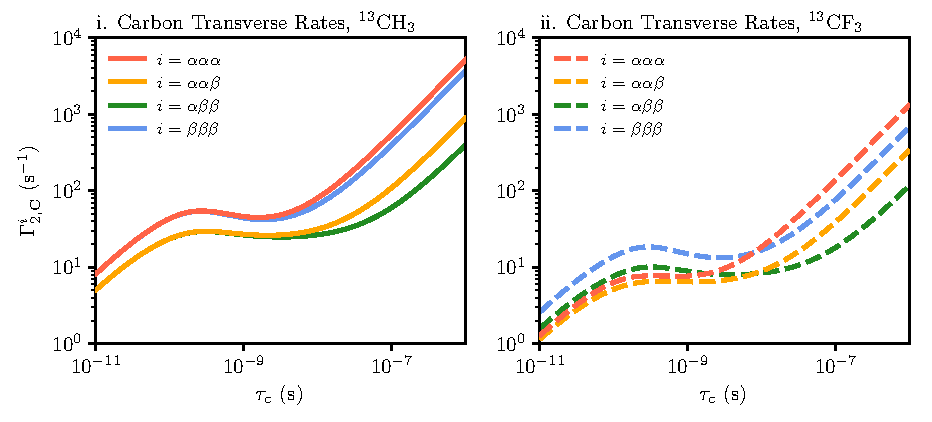
\includegraphics[scale=0.9]{./Figures/SimonsFigs/CvF.pdf}
\caption{Plots of transverse $^{13}$C relaxation rates versus global tumbling correlation time, $\tau_{\text{c}}$, for $^{13}$CH$_3$ and $^{13}$CF$_3$, using the Woessner Model. Parameters used: $B_0 = \num{14.1} \si{\tesla}$, $\gamma_{\text{C}} = \num{67.283e6} \si{\radian \per \second \per \tesla}$, $\gamma_{\text{H}} = \num{267.513e6} \si{\radian \per \second \per \tesla}$, $\gamma_{\text{F}} = \num{251.662e6} \si{\radian \per \second \per \tesla}$, $r_{\text{CH}} = r_{\text{HH}} = \num{1.09} \si{\angstrom}$, $r_{\text{CF}} = r_{\text{FF}} = \num{1.33} \si{\angstrom}$, $\beta = \ang{109.47}$, $\tau_{\text{m}} = \num{50} \si{\pico \second}$, $\Delta \sigma_{\text{C}} = \num{20} \text{ppm}$, $\Delta \sigma_{\text{H}} = \num{1} \text{ppm}$, $\Delta \sigma_{\text{F}} = \num{140} \text{ppm}$. A single external proton was considered, at an average distance of $\num{3} \si{\angstrom}$ from the $^1$H/$^{19}$F nuclei.}
\label{CvF}
\end{figure}
The major cause of the reduced $^{13}$CF$_3$ rates, relative to methyl is due to differences in dipolar couplings. The distances between the nuclei in the $^{13}$CF$_3$ moiety ($\num{1.33} \si{\angstrom}$) were set to be larger relative to the $^{13}$CH$_3$ distances ($\num{1.09} \si{\angstrom}$). Also, the gyromagnetic ratio of $^{19}$F is slightly smaller than that of $^1$H. These factors result in weaker dipolar interactions between the trifluoromethyl spins. The implication of these plots is that dipolar interactions are still the dominant relaxation-inducing mechanism in $^{13}$CF$_3$, despite the significantly elevated magnitude of the I-spin CSA. The impact of the $^{19}$F CSA should however be augmented as the magnetic field strength is increased\footnote{It can be seen from \ref{DipConst} and \ref{CSAConst} that $c_{\text{I}} \propto B_0$, whilst the dipolar constant, $d_{\text{IS}}$ has no dependence on $B_0$. Consequently, as $B_0$ is increased, the ratios $|\frac{c_{\text{I}}}{d_{\text{IS}}}|$ and $|\frac{c_{\text{I}}}{d_{\text{II}}}|$ will increase.}.
\subsection{Effect of Field Strength on $^{13}$CF$_3$ Rates}
NMR spectrometers operating at $^1$H Larmor frequencies of the order of gigahertz now exist, though these are not particularly commonplace at the time of writing. In order to assess the impact of higher field strengths on $^{13}$CF$_3$ relaxation rates, calculation ii. in Figure \ref{CvF} (corresponding to transverse $^{13}$C rates) was repeated, with $B_0$ set to $\num{23.49} \si{\tesla}$ (corresponding to a $\num{1} \si{\giga \myhertz}$ spectrometer).\\
\begin{figure}
\centering
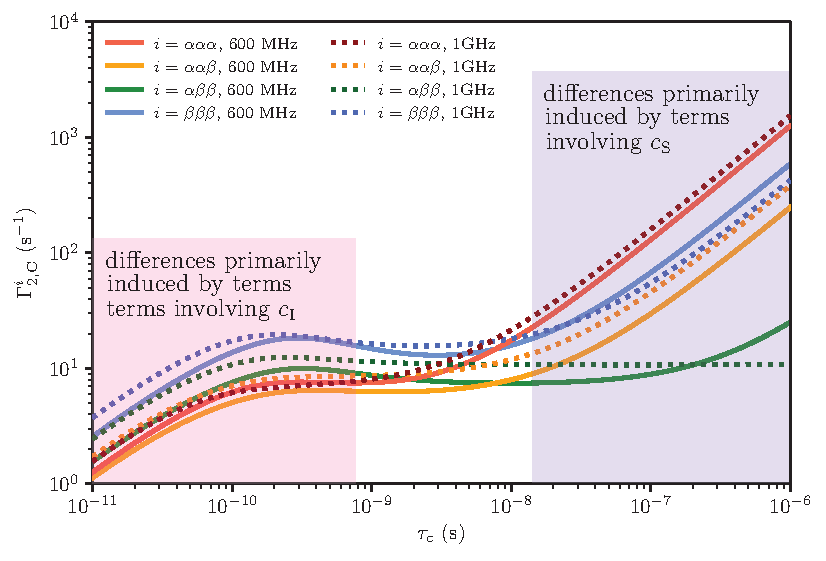
\includegraphics[scale=1]{./Figures/SimonsFigs/13CF3_1000.pdf}
\caption{Plots of $^{13}$C transverse relaxation rates, for a $^{13}$CF$_3$ moiety, using the Woessner Model. Two different field strengths were considered: $B_0 = \num{14.10} \si{\tesla}$ and $B_0 = \num{23.49} \si{\tesla}$, corresponding to $\num{600} \si{\mega \myhertz}$ and $\num{1} \si{\giga \myhertz}$ spectrometers, respectively. Parameters used: $\gamma_{\text{C}} = \num{67.283e6} \si{\radian \per \second \per \tesla}$, $\gamma_{\text{F}} = \num{251.662e6} \si{\radian \per \second \per \tesla}$, $r_{\text{CF}} = r_{\text{FF}} = \num{1.33} \si{\angstrom}$, $\theta = \ang{109.47}$, $\tau_{\text{m}} = \num{50} \si{\pico \second}$, $\Delta \sigma_{\text{C}} = \num{20} \text{ppm}$, $\Delta \sigma_{\text{F}} = \num{140} \text{ppm}$.}
\label{13CF3_1000}
\end{figure}
There are changes to all the relaxation rates when $B_0$ is increased, as can be seen in Figure \ref{13CF3_1000}. This indicates that chemical shift anisotropy effects are becoming more influential, as is to be expected. Yet even at the higher field strengths, dipolar effects are dominating the relaxation behaviour. Close inspection of the components in the rate expressions reveal that terms proportional to $c_{\text{I}}^2$ and $d_{\text{II}} c_{\text{I}}$ do have an impact on the rates when faster molecular tumbling is considered (i.e. small $\tau_{\text{c}}$). Despite this, as $\tau_{\text{c}}$ is increased, the impact of the $^{19}$F CSA becomes less significant. This is since none of the terms involving $c_{\text{I}}$ possess spectral densities with frequency $0$. The primary term causing the deviation in rate with field strength in the macromolecular limit is proportional to $d_{\text{IS}}c_{\text{S}} J\left(\tau_{\text{c}}, 0\right) = d_{\text{IS}}c_{\text{S}} \tau_{\text{c}}$. It is therefore the $^{13}$C CSA, coupled with the $^{13}$C-$^{19}$F dipolar interactions, that is driving the change in rates to the right hand side of Figure \ref{13CF3_1000}.\\
The calculations above indicate that the $^{19}$F CSA does not have a noticeable impact on $^{13}$C transverse relaxation rates in the macromolecular limit. Despite this, it may well be more influential when the relaxation of other coherences is considered. Any coherence for which the relaxation rate has a dependence on $A_1 A_2 J(\tau_{\text{c}},0)$, where $A_1$ and/or $A_2$ are $c_{\text{I}}$, is likely to be heavily influenced by the $^{19}$F CSA in the macromolecular limit. Significant deviations in behaviour relative to $^{13}$CH$_3$ systems are likely for such coherences, on top of the differences in dipolar contributions. Nevertheless, the calculations shown above provide strong evidence that the $^{13}$CF$_3$ moiety is likely to be an effective probe in an appropriate TROSY experiment, due to the low relaxation rates predicted relative to $^{13}$CH$_3$.
\subsection{The $\alpha \beta \beta$ Line}
The behaviour of the $\alpha \beta \beta$ line at high field strength deserves consideration. From Figure \ref{13CF3_1000}, the rate of this coherence plateaus in the macromolecular limit at sufficiently high field strength. The cause of this is an almost perfect cancellation of the terms in the expression for $\Gamma_{2,\text{S}}^{\alpha\beta\beta}$ (see Equation \ref{MacroLim}). This result already hints at a potential coherence that could be targeted via a $^{13}$CF$_3$ TROSY technique. Generation of $^{13}$C single quantum coherence, and subsequent selection of the $\alpha \beta \beta$ peak may well lead to highly intense spectra. Such selection processes exist, including a method introduced by Kontaxis and Bax\cite{RN3}.

% Report-ExperimentalRelaxationInvestigations.tex
% Simon Hulse
% simonhulse@protonmail.com
% Last Edited: Wed 27 Nov 2024 02:43:47 PM EST

% !TeX root = ./Report-Body.tex
\chapter{Experimental Relaxation Investigations}
In an attempt to gain an in-depth understanding of methyl relaxation, a series of NMR experiments were conducted on a test compound over a range of temperatures. By varying temperature, the viscosity of the medium in the NMR tube changes. As such, doing this provides a means of monitoring relaxation rates as function of rotational correlation time, $\tau_{\text{c}}$. The molecule considered in these studies is shown in Figure \ref{TransverseSpectra}. This was present in a highly viscous medium composed of $95 \%$ d-glycerol and $5 \%$ d-DMSO. The intention was for this simple, small molecule to mimic the motional behaviour typical of molecules far larger that it.
\section{Experiments Conducted}
Transverse $^{13}$C relaxation experiments were carried out to determine the four rates, $\Gamma_{2,\text{C}}^{i}$ (discussed in the previous chapter), experimentally. Furthermore, $^1$H translational diffusion experiments were conducted, which can be used as a gauge of the molecule's motional behaviour. All Experiments were carried out on a Varian $\num{600} \si{\mega \myhertz}$ spectrometer. Spectra were processed using NMRPipe\cite{RN43}.\\
\subsection{$^{13}$C Transverse Relaxation Experiment}
\begin{figure}
\centering
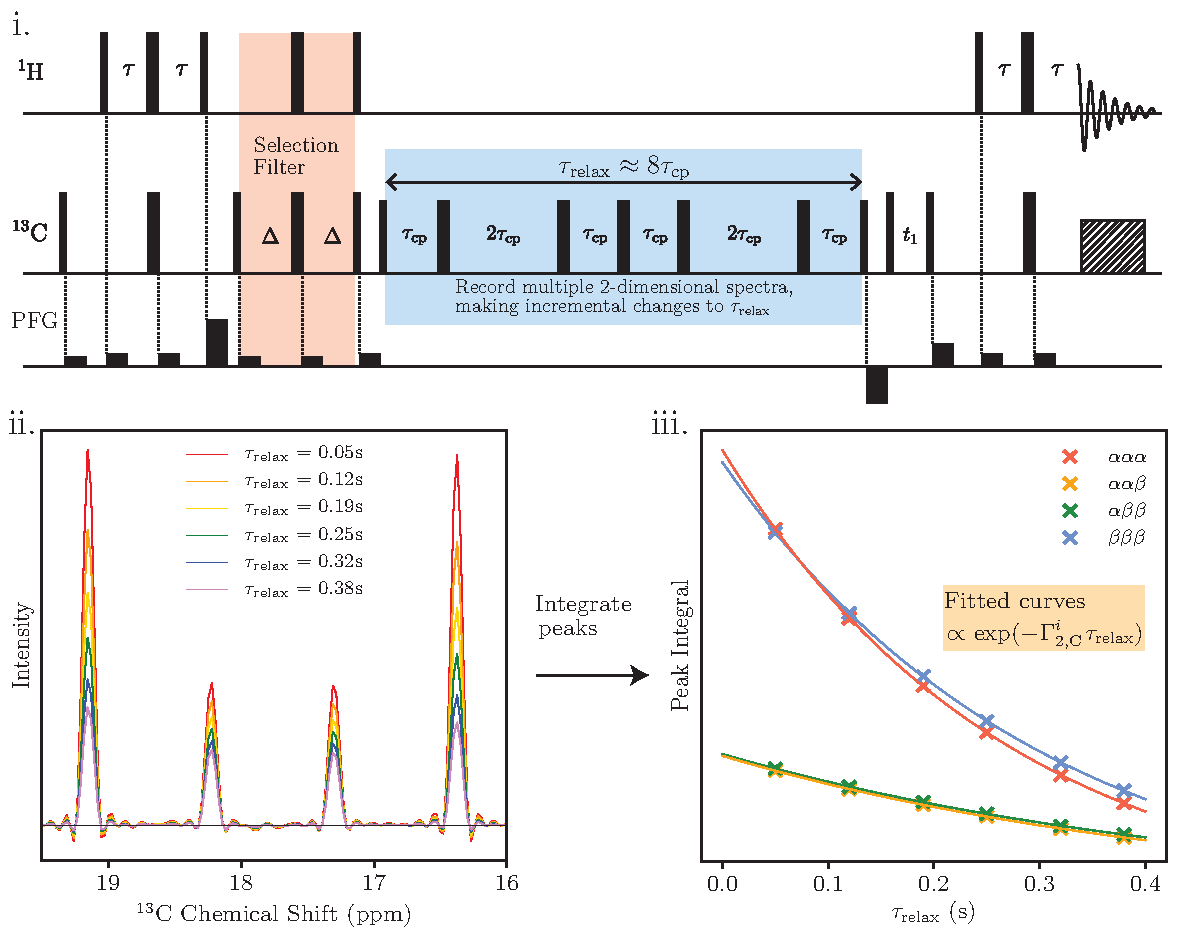
\includegraphics[scale=0.75]{./Figures/SimonsFigs/DecayCurves.pdf}
\caption{i. The pulse sequence used to determine $^{13}$C transverse relaxation rates. ii. A cross section through a $^{13}$C quartet, of two-dimensional spectra obtained using the pulse sequence. As $\tau_{\text{relax}}$ is increased, the intensity of the peaks in the quartet decreases. Individual peaks in each spectrum are integrated, and these integrals are plotted as a function of $\tau_{\text{relax}}$, iii. Fitting exponential curves to each set of points allows extraction of relaxation rates of each coherence at a given temperature. The experiment is then repeated using a range of temperatures to determine how relaxation rates vary with viscosity.}
\label{RelaxDecay}
\end{figure}
The acquisition of experimental values for $\Gamma_{2,S}^i$ was achieved using the pulse sequence in Figure \ref{RelaxDecay}.i. $^{13}$C single-quantum coherences were generated via use of an INEPT sequence\cite{RN54}, and subsequently allowed to evolve for a specified period of time, $\tau_{\text{relax}}$. The pulse sequence used has many similarities with a conventional HSQC pulse sequence, shown in Figure \ref{HSQCHMQC}.ii. Two major elements are added to the sequence, enabling relaxation rate studies:
\begin{itemize}
\item A selection filter (highlighted in red), devised by Kontaxis and Bax\cite{RN3}. Varying the value of the time delay $\Delta$, and taking linear combinations of spectra enables the isolation of a single peak within the methyl quartet.
\item A Carr-Purcell-Meiboom-Gill (CPMG) element\cite{RN47,RN48} (highlighted in blue), during which the desired coherences are allowed to relax.
\end{itemize}
By obtaining a series of spectra\footnote{The spectra in Figure \ref{RelaxDecay}.ii. adopt an approximate intensity ratio of 3:1:1:3, at least for smaller $\tau_{\text{relax}}$ values. This contrasts with what is typical of a 1D $^{13}$C spectrum, where a 1:3:3:1 intensity ratio results. This intensity ratio manifests as a result of the way the magnetisation evolves during the HSQC pulse sequence\cite{RN49}} with differing values of $\tau_{\text{relax}}$, and integrating the resultant peaks, a decay profile is obtained. The relaxation rate of each coherence is calculated by fitting an exponential function to the decay profile. Repetitions of this experiment were then carried out, at different temperatures.\\
\begin{figure}
\centering
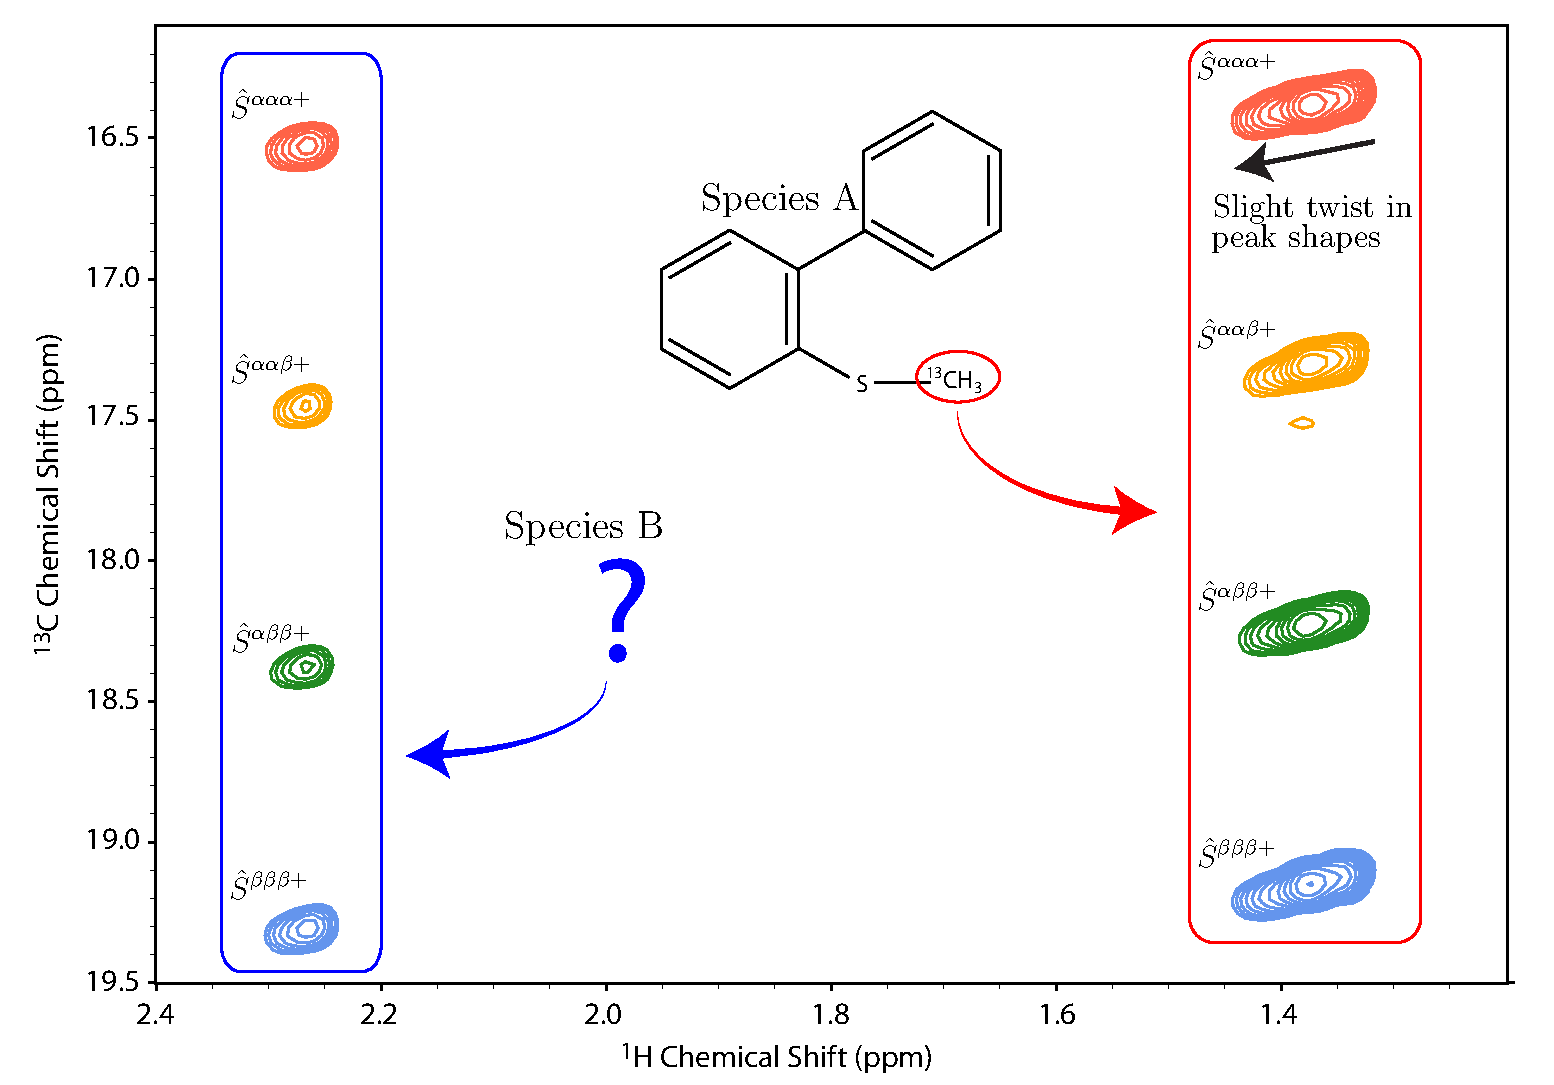
\includegraphics[scale=0.5]{./Figures/SimonsFigs/13CTransExptSpectrum.pdf}
\caption{An example of a spectrum obtained using the $^{13}$C transverse relaxation experiment. The spectrum were taken at $T = \num{30}^{\circ}\text{C}$, with $\tau_{\text{relax}} = \num{0.05} \si{\second}$. Two distinct chemical environments are present in the spectrum, indicating two species, A and B, are present.}
\label{TransverseSpectra}
\end{figure}
Figures \ref{TransverseSpectra} shows an example spectrum obtained using the $^{13}$C transverse relaxation experiment. The expected spectrum of a molecule with one $^{13}$CH$_3$ moiety is a single quartet. Curiously, the spectra obtained instead comprised two separate quartets. The implication of this is that two distinct chemical species, each possessing $^{13}$CH$_3$ moieties, were present in the sample (which will be referred to as A and B). This was a rather fortuitous outcome, as it enabled the acquisition of a larger data set.\\
The peak shapes exhibited a slightly twisted geometry in the spectra, as is indicated in Figure \ref{TransverseSpectra}, which was probably due to isotope-shift effects.\\
\subsection{Diffusion Experiments}
Diffusion NMR experiments measure the attenuation of a sample's signal, via the application of pulsed field gradients (PFGs)\cite{RN51}. Larger molecules, which translate slowly in solution, suffer less signal attenuation with increasing gradient strength, relative to smaller, more rapidly translating molecules. Measuring signal intensity as a function of gradient strength, and fitting the data using the Stejskal-Tanner equation\cite{RN42} provides a means of determining the translational diffusion constant, $D$, of the various species in an NMR sample.\\
1D proton diffusion experiments were conducted on the sample, at varying temperatures. It was possible to determine translational diffusion constants for both species A and B. As well as this, diffusion data for the glycerol could also be obtained.
\section{Fitting Relaxation Models to the Data}
The ability of the Woessner and diffusive models to describe the data was assessed using a least squares fitting procedure. The solution of a least squares procedure is that which minimises the summation of squared residuals, commonly denoted $\chi^2$:
\begin{equation}
\chi^2 = \sum \limits_i (y_{i,\text{data}} - y_{i,\text{fit}})^2
\end{equation}
A least squares procedure to globally optimise the parameters $\Delta \sigma_{\text{I}}$, $\Delta \sigma_{\text{S}}$ and $\tau_{\text{m}}$ was performed, using both the Woessner and diffusive models. To incorporate the effect of external protons in the molecule into the fit, it was assumed that a single proton existed, separated from the methyl protons by a distance $r_{\text{ext}}$. The value of $r_{\text{ext}}$ was also included in the fitting procedure. On top of globally fitting the aforementioned parameters, $\tau_{\text{c}}$ was optimised at each temperature (locally). Fits in which $\tau_{\text{m}}$ were set to be local were also carried out. It was found that the $\chi^2$ values of fits incorporating local and global $\tau_{\text{m}}$ were very similar, which lead to the decision to fit it globally. One major difference between the Woessner and diffusive models is the temperature dependence of methyl rotation. In the Woesnner model, the protons undergo activationless jumps, and hence exhibit no temperature dependence. Conversely $\tau_{\text{m}}$ is anticipated to vary with temperature if the diffusive model is obeyed, as an activation barrier to the motion is present. The lack of any significant local dependence of $\tau_{\text{m}}$ is evidence in favour of the Woessner model.\\
In order to determine errors for the fitting parameters, a bootstrapping method was applied. This method relies on taking a random sample of data points from the complete data set, allowing repetition of points, and performing the same optimisation procedure again. This process is then repeated multiple times. In the limit of infinite runs, it is anticipated that the mean of the distribution of values determined for a particular parameter will converge on its true value. The standard deviation in values of the bootstrap acts as measure of the error in the fitting parameter.
\subsection{Species A}
\begin{figure}
\centering
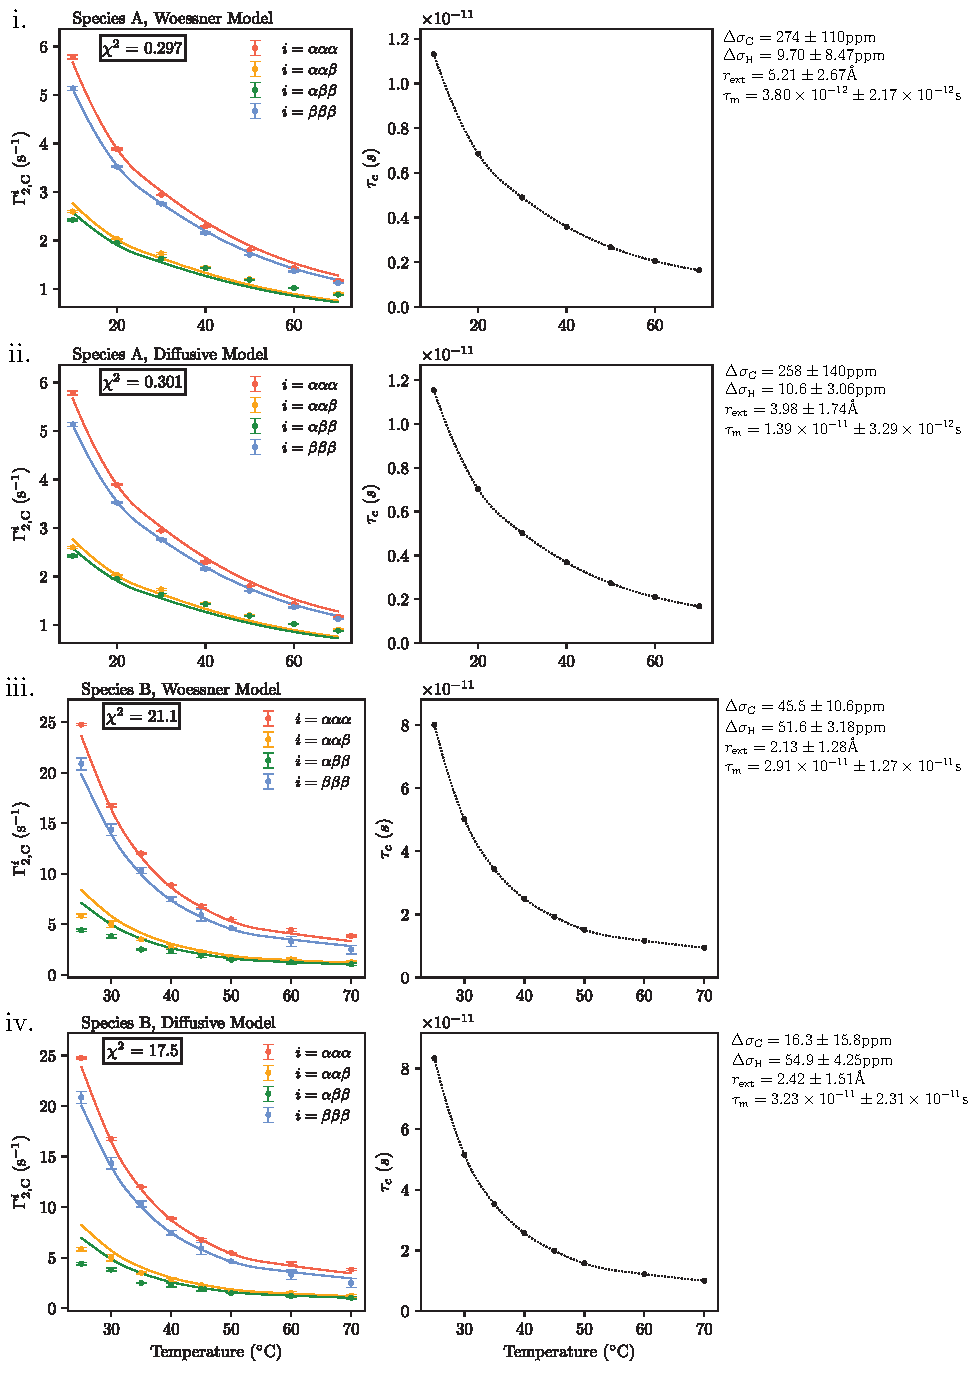
\includegraphics[scale=0.9]{./Figures/SimonsFigs/Fits.pdf}
\caption{Results of a least squares fitting procedure, using both the Woessner and diffusive models, applied to the $^{13}$C transverse relaxation rate data acquired.}
\label{Fits}
\end{figure}
Plots i. and ii. in Figure \ref{Fits} show the results of the least squares procedure applied to species A, using both the Woessner and diffusive models. The $\chi^2$ values obtained show a close agreement between the models. Also, the values of the fitted parameters were found to be highly similar. This meant there was very little scope to compare the two models. The $\tau_{\text{{c}}}$ values obtained imply that the molecule is undergoing rapid tumbling, and is certainly not adhering in the macromolecular limit. The $^{13}$C CSA is predicted to be very large by the fitting procedure. Typical methyl $^{13}$C CSA values are between 17-25ppm, for Ile and Val\cite{RN50}. Though this may be anticipated to be slightly higher when the methyl group is adjacent to a sulfur atom, an increase of 2 orders of magnitude is unlikely.  Plots i. and ii. in Figure \ref{CH3Models} provide predictions of relaxation rates made by the models, using parameters which are typical for a methyl moiety. It can be seen that the relaxation rates of the two outer ($\alpha \alpha \alpha$ and $\beta \beta \beta$) lines are virtually identical in the fast tumbling regime. Despite this, noticeable differences are observed in the acquired data. The fitting procedure has accounted for this split in the rates by setting $\Delta \sigma_{\text{C}}$ to be very large.
\subsection{Species B}
The analogous results of the fitting procedure for species B are shown in iii. and iv. of Figure \ref{Fits}. In this case, the diffusive model did seem to produce a slightly better fit, relative to the Woessner model, though again, the difference was very minor.
\section{Comparing Diffusion Data with Relaxation Data}
Predictions of the hydrodynamic radii, $r_{\text{H}}$, of the species were carried out, by implementation of the Stokes-Einstein equation:
\begin{equation}
\label{Stokes}
r_{H} = \frac{k_{\text{B}}T}{6\pi \eta D}
\end{equation}
where $k_{\text{B}}$ is the Boltzmann constant, and $\eta$ is the viscosity of the medium. The viscosity of the medium was calculated over the range of temperatures considered, by use of an empirically determined model, and assuming the medium was comprised of pure glycerol\cite{RN52}.\\
\begin{figure}
\centering
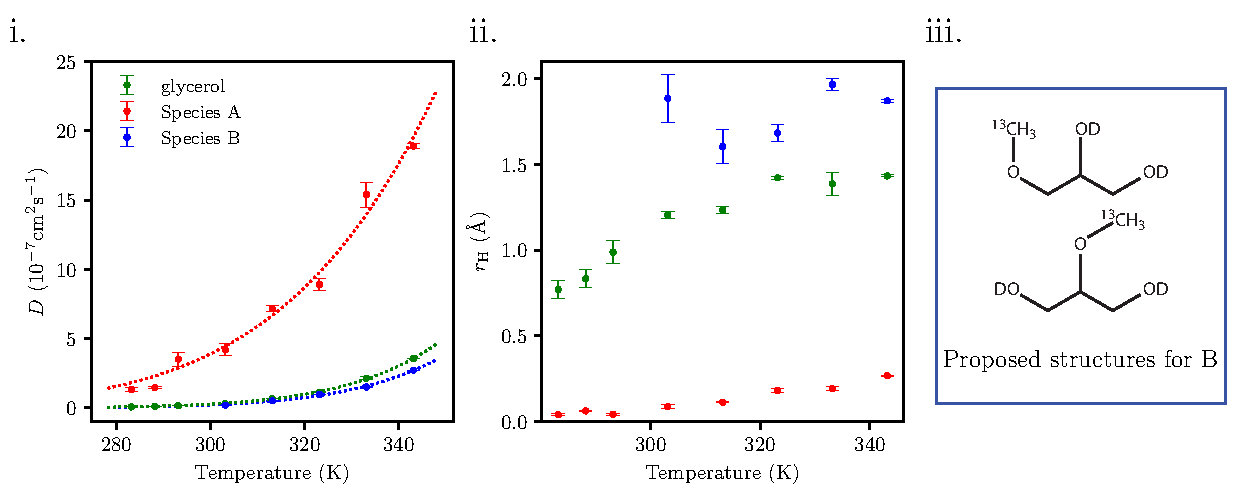
\includegraphics[scale=0.7]{./Figures/SimonsFigs/Diffusion.pdf}
\caption{i. Plots of translational diffusion constant, $D$, versus temperature for species A, species B, and glycerol. Arrhenius-type fits of the form $D = A\exp(-\frac{B}{T})$ were generated for each species. ii. Calculated hydrodynamic radii, $r_{\text{H}}$, for the three species as a function of temperature. iii. By noting that the diffusion constants of species B and glycerol are very closely matched, it is proposed that either of the structures shown could correspond to species B.}
\label{Diffusion}
\end{figure}
From the data in Figure \ref{Diffusion}.i., species A was found to be diffusing far more rapidly than both the glycerol and species B. This implies that species A is able to translate in an unrestricted fashion, without too much hindrance from the viscous medium it is in. The hydrodynamic radii across all temperatures were calculated to be on the order of $\num{E-11} \si{\meter}$, which is far smaller than anticipated for a molecule of its size. On account of this, along with the very small rotational correlation times predicted from the relaxation rate fits, it is postulated that the molecule is diffusing through the medium in a highly anisotropic, 'bullet-like' fashion, as would be expected of a prolate spheroid.\\
In order to assess this prediction, the rotational correlation times extracted from our fitted Woessner model was compared with the hydrodynamic data obtained of species A. The following expression relates the rotational correlation time with the hydrodynamic radius of the molecule\cite{RN56}:
\begin{equation}
\label{TaucRH}
\tau_{\text{c}} = \lambda\frac{4 \pi \eta r_{\text{H}}^3}{3k_{\text{B}}T}
\end{equation}
$\lambda$ is a constant that indicates deviation from spherical behaviour. For a perfect sphere, it is predicted that $\lambda = 1$. Using \ref{Stokes} and \ref{TaucRH}, the following expression for $\lambda$ can be obtained, in terms of the hydrodynamic radius of glycerol, and the diffusion constants of glycerol and species A:
\begin{equation}
\lambda = \frac{4 r_{\text{H,gly}}^2 D_{\text{gly}}^2}{18D_{\text{A}}^3}
\end{equation}
A plot of $\lambda$ versus temperature is shown in Figure \ref{Lambda}. The values of $\lambda$ show a decline with temperature, but for the most part they are comfortably above 1, which acts to validate the proposal that the molecule is not undergoing spherical motion.
\begin{figure}
\centering
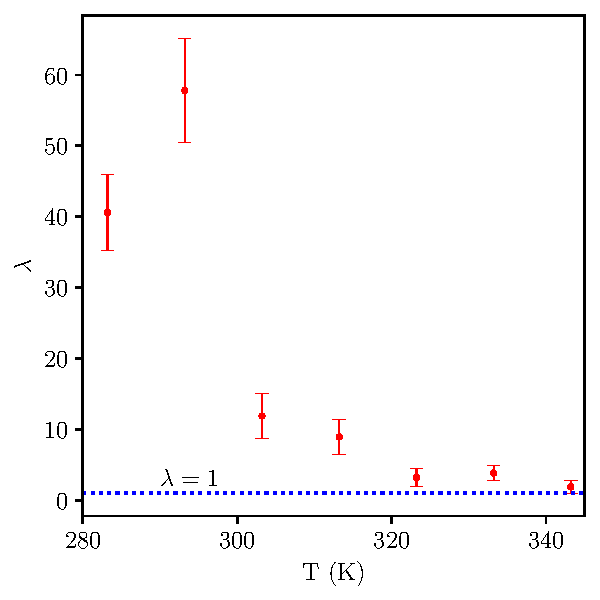
\includegraphics[scale=0.7]{./Figures/SimonsFigs/Lambda.pdf}
\caption{A plot of $\lambda$ versus $T$ for species A. A decline in the value of $\lambda$ is found with increasing temperature, indicating that the molecule's motion is becoming less anisotropic as the viscosity of glycerol decreases.}
\label{Lambda}
\end{figure}
Figure \ref{AnisotropicMotion} illustrates how we anticipate this molecule behaves within the medium. First, it is able to translate far more effectively in one dimension that the other two, following a largely linear path. As well as this, the global rotation of the molecule about its major axis is less hindered by the medium, relative to rotation about its other axes. In order to effectively account for anisotropic tumbling, it would be necessary to redefine the spectral density function which describes the global motion. Accounts of spectral densities for anisotropic motions are well documented in the literature, with the relevant expression for a prolate spheroid being the following\cite{RN53}:
\begin{equation}
J(\omega) = \frac{1}{4}\left(3\cos^2\theta-1\right)^2 \frac{\tau_{\text{A}}}{1+ \omega^2\tau_{\text{A}}^2} + 3\sin^2\theta\cos^2\theta \frac{\tau_{\text{B}}}{1+ \omega^2\tau_{\text{B}}^2} + \frac{3}{4}\sin^4\theta\frac{\tau_{\text{C}}}{1+ \omega^2\tau_{\text{C}}^2}
\end{equation}
with the correlation times $\tau_{\text{A}}, \tau_{\text{B}}, \tau_{\text{C}}$ depending on the rotational diffusion constants perpendicular and parallel to the spheroid's axis of symmetry ($D_{\perp}$ and $D_{\parallel}$). It is highly plausible that an additional component of motion is also in effect: the rotation of the methyl threefold axis, characterised by correlation time $\tau_{\text{axis}}$. As mentioned earlier in this thesis, this motion has been incorporated into relaxation models via a model-free approach\cite{RN31}.\\
\begin{figure}
\centering
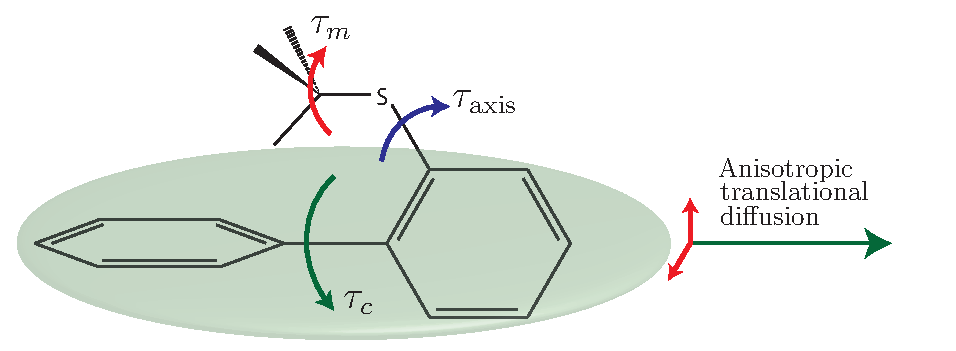
\includegraphics[scale=0.8]{./Figures/SimonsFigs/SpeciesAMotion.pdf}
\caption{The proposed types of motion adopted by species A within the glycerol medium. Anisotropic translational and rotational diffusion are both acting, as would be expected of a prolate spheroid. The uncorrelated motion of the methyl symmetry axis may also feature.}
\label{AnisotropicMotion}
\end{figure}
Species B exhibits very similar diffusion properties to glycerol, as seen in Figure \ref{Diffusion}. This provides evidence that species B is formed as the product of a reaction between glycerol and species A. Potential structures of species B, which fit this hypothesis are shown in Figure \ref{Diffusion} iii., though further studies to gain clarity on this matter were not carried out.
\section{Summary of Experimental Results}
The results obtained from fitting our models show that our theory is able to describe the $^{13}$C relaxation rate data effectively. The temperature independence of $\tau_{\text{m}}$ that is observed from the fitting procedure points to the Woessner model as the more effective of the two at describing methyl relaxation phenomena. The test molecule, which was hoped to mimic proteins by being present in a highly viscous medium, never left the small molecules limit. This is accounted for by noting it travelled in a highly anisotropic, 'bullet-like' fashion. The motion became more isotropic as the viscosity of the glycerol increased, as evidenced by a decrease in $\lambda$ with temperature.

% Report-ConclusionsFutureWork.tex
% Simon Hulse
% simonhulse@protonmail.com
% Last Edited: Wed 27 Nov 2024 02:30:08 PM EST

% !TeX root = ./Report-Body.tex
\chapter{Conclusions and Future Work}

\section{Conclusions}
In this thesis, a novel relaxation model, describing I$_3$S spin-systems has
been presented. This model is applicable to all molecular motion regimes, which
is one of its stand-out advantages over other models presented. As well as
this, via incorporation of I-spin CSA contributions, it is well-equipped to
describe relaxation in $^{13}$CF$_3$ spin systems.

Utilising this theory, calculations comparing relaxation phenomena in $^{13}$CH$_3$ and $^{13}$CF$_3$ moieties predict that there are significant advantages in using trifluoromethyl moieties over methyls. This is on account of the slower relaxation rates of the coherences considered. Favourable behaviour in $^{13}$CF$_3$ can largely be accounted for by a geometry-driven reduction in the magnitude of dipolar couplings between spins. The $^{19}$F CSA is also capable of having a noticeable impact on rates as well.

An attempt to mimic a protein using our test system had limited success. Via hydrodynamic considerations, it was ascertained that the test molecule was able to move very rapidly though the glycerol medium. The motion it adopts is highly anisotropic, with its translational behaviour being 'bullet-like'. Nonetheless, fits of our proposed relaxation models to the rate data obtained illustrate that we have a strong handle on relaxation. Our investigation supports a Woessner-type hopping combined with anisotropic rotation of our test molecule, due to the seeming lack of temperature dependence on methyl tumbling.

\section{Future Work}
The results of the calculations presented in this thesis provides motivation to proceed with the development of an NMR methodology that uses $^{13}$CF$_3$ moieties as probes in large biomolecules. For such a methodology to be realised, further work will still be required in two principle areas.

In order for a $^{13}$CF$_3$ TROSY experiment to become a well-established technique, a method of incorporating this spin-label into proteins is necessary. Work on this is currently being undertaken by research groups in collaboration with the Badlwin group, with promising results starting to emerge\cite{RN55,RN19}.

Establishing a rigorous understanding of relaxation in I$_3$S spins systems has opened up the possibility to evaluate a pulse sequence's effectiveness on $^{13}$CF$_3$ moieties. Via density matrix calculations, simulations of NMR experiments will provide a route to determining an optimal $^{13}$CF$_3$ TROSY experiment. This will hopefully enable studies of biomolcules that are currently out of our grasp using NMR.

% !TeX root = ./Report-Body.tex
%%% You do not need to edit this file.
\begingroup%
\makeatletter\if@tightbibliography%
\let\normalsize\footnotesize%
\singlespacing%
\fi%
\chapter*{\bibname}%
%\phantomsection%
\addcontentsline{toc}{chapter}{\bibname}%
\printbibliography[segment=0,resetnumbers=true,heading={mainbib}]%
\endgroup%
\appendix% Comment out if you don't need it.
% !TeX root = ./Report-Body.tex
\chapter{Bloch-Redfield-Wangsness Theory}

\begin{appendixtext}
In this appendix, I present a derivation of the relaxation superoperator, $\hat{\hat{\Gamma}}$, using BWR theory. First,  a general approach to time-dependent perturbation theory is considered, which is subsequently applied to the specific case of an ensemble of systems, each described by a density matrix, $\hat{\rho}$. The approach I adopt in section \ref{secA.2} follows closely to previous accounts, such as those given by Goldman and Palmer$^{\text{[1,2]}}$\\
\section{Second order perturbation theory} \label{secA.1}
The Schr\"{o}dinger Equation involving a time-dependent Hamiltonian is given by:
\begin{equation}
\label{eqA.1}
\pdv{\ket{\psi(t)}}{t}=-i\hat{H}(t)\ket{\psi(t)}
\end{equation}
Expressing this in integrated form:
\begin{equation}
\label{eqA.2}
\ket{\psi(t)}=\ket{\psi(0)}-i\int_0^t \hat{H}(t^{\prime})\ket{\psi(t^{\prime})} dt^{\prime}
\end{equation}
Inputting the result of \ref{eqA.2} into the right-hand side of \ref{eqA.1} leads to the following expression:
\begin{equation}
\label{eqA.3}
\pdv{\ket{\psi(t)}}{t}=-i\hat{H}(t)\left[\ket{\psi(0)}-i\int_0^t \hat{H}(t^{\prime})\ket{\psi(t^{\prime})} \right]dt^{\prime}
\end{equation}
Integrating again obtains:
\begin{equation}
\label{eqA.4}
\ket{\psi(t)}=\ket{\psi(0)}-i\ket{\psi(0)}\int_0^t \hat{H}(t^{\prime}) dt^{\prime}-\int_0^t \hat{H}(t^{\prime}) \int_0^{t^{\prime}}\hat{H}(t^{\prime\prime})\ket{\psi(t^{\prime\prime})} dt^{\prime\prime} dt^{\prime}
\end{equation}
If we continue to repeat this procedure of inserting into \ref{eqA.1} and integrating, we arrive at:
\begin{equation}
\label{eqA.5}
\begin{split}
&\ket{\psi(t)}=\left[\sum\limits_{n=0}^\infty \hat{I}_n(t)\right]\ket{\psi(0)} \\
&\hat{I}_n(t)=(-i)^n\int_0^t dt^{\prime}\int_0^{t^{\prime}} dt^{\prime\prime}...\int_0^{t^{{(n-1)}^{\prime}}} dt^{n^{\prime}}\hat{H}(t^{\prime})\hat{H}(t^{\prime\prime})...\hat{H}(t^{n^{\prime}})
\end{split}
\end{equation} 
The essence of second order perturbation theory is to truncate this expression, removing any terms of order higher than 2, such that:
\begin{equation}
\label{eqA.6}
\ket{\psi(t)}=\left[1-i\int_0^t \hat{H}(t^{\prime}) dt^{\prime}-\int_0^t  \int_0^{t^{\prime}} \hat{H}(t^{\prime})\hat{H}(t^{\prime\prime}) dt^{\prime\prime} dt^{\prime}\right]\ket{\psi(0)}
\end{equation}

\section{Derivation of the relaxation superoperator} \label{secA.2}
Now we will apply the result obtained above to the Liouville-von Neumann equation, which describes the evolution of the density matrix $\hat{\rho}(t)$ in Liouville space:
\begin{equation}
\label{eqA.7}
\pdv{\hat{\rho}(t)}{t}=-i\hat{\hat{H}}(t)\hat{\rho}(t)
\end{equation}
where $\hat{\hat{H}}(t)$ is the commutation superoperator of $\hat{H}(t)$:
\begin{equation}
\label{eqA.8}
\hat{\hat{H}}(t)=\comm{\hat{H}(t)}{}
\end{equation} 
To proceed, we split $\hat{\hat{H}}(t)$ two parts. The first, $\hat{\hat{H}}_0$ contains all the static, time independent components of the Hamiltonian. For our purposes, this will include contributions such Zeeman interaction, isotropic chemical shift, scalar coupling, and so on. The second term, $\hat{\hat{H}}_1(t)$, contains all the stochastic time dependent terms, which arise due to molecular motion. Anisotropic contributions, such as those from the dipolar interaction and chemical shift anisotropy will be contained within this.
Hence the Liouville-von Neumann equation becomes
\begin{equation}
\label{eqA.9}
\pdv{\hat{\rho}(t)}{t}=-i\left[\hat{\hat{H}}_0+\hat{\hat{H}}_1(t)\right]\hat{\rho}(t)
\end{equation}
The form $\hat{\hat{H}}_1 (t)$ takes is that of randomly fluctuating noise, which is not reproducible nor differentiable. We therefore wish to seek an expression not explicitly in terms of $\hat{\hat{H}}_1 (t)$, but instead in terms of it's statistical properties, which are well defined. It therefore seems natural to proceed using the perturbation theory derived in the previous section.\\
There many assumptions used in this derivation, some of which are as follows:
\begin{itemize}
\item The noise is assumed to be stationary, i.e. it may well vary randomly with time, but it's statistical properties do not depend on the time point being considered
\item The ensemble average of $\hat{\hat{H}}_1 (t)$ is zero. i.e: $\overline{\hat{\hat{H}}_1 (t)}=0$.
\item $\norm{\hat{\hat{H}}_1(t)}\ll\norm{\hat{\hat{H}}_0}$, i.e the relative "size" of $\hat{\hat{H}}_1(t)$ is small compared with $\hat{\hat{H}}_0$. This is a necessity for the perturbation theory to be valid.
\end{itemize}
Before applying perturbation theory to \ref{eqA.9}, we shall change the reference frame, to one called the interaction frame with respect to $\hat{H}_0$, which is achieved as follows:
\begin{equation}
\label{eqA.10}
\hat{\rho}^I(t)=e^{i\hat{\hat{H}}_0t}\hat{\rho}(t)\quad\text{and}\quad\hat{\hat{H}}_1^I(t)=e^{i\hat{\hat{H}}_0t}\hat{\hat{H}}_1(t)e^{-i\hat{\hat{H}}_0t}
\end{equation}
we can utilise \ref{eqA.9} to derive the following expression for the time evolution of the density matrix in the interaction frame:
\begin{equation}
\label{eqA.11}
\pdv{\hat{\rho}^I(t)}{t}=-i\hat{\hat{H}}_1^I(t)\hat{\rho}^I(t)
\end{equation}
where the superscript $I$ refers to said interaction frame. \\
It should be noted that the influence of $\hat{\hat{H}}_0$ has vanished; this has been incorporated into the definition of the density matrix. This transformation gets rid of the very large contribution from $\hat{\hat{H}}_0$, allowing consideration of longer time scales than would be the case without such a transformation. \\
Applying seond order perturbation theory to \ref{eqA.11} results in the following expression:
\begin{equation}
\label{eqA.12}
\pdv{\hat{\rho}^I(t)}{t}=-i\hat{\hat{H}}_1^I(t)\hat{\rho}^I(0)-\int_0^t \hat{\hat{H}}_1^I(t)\hat{\hat{H}}_1^I(t^{\prime})\hat{\rho}^I(t^{\prime}) dt^{\prime}
\end{equation}
Applying an ensemble average to the expression:
\begin{equation}
\label{eqA.13}
\pdv{\overline{\hat{\rho}^I(t)}}{t}=-i\overline{\hat{\hat{H}}_1^I(t)\hat{\rho}^I(0)}-\int_0^t \overline{\hat{\hat{H}}_1^I(t)\hat{\hat{H}}_1^I(t^{\prime})\hat{\rho}^I(t^{\prime})} dt^{\prime}
\end{equation}
Recall from one of the assumptions above, that $\overline{\hat{\hat{H}}_1(t)}=0$. Using the definition of $\hat{\hat{H}}_1^I(t)$ in \ref{eqA.10}, and noting that $\hat{\hat{H}}_0$ is time independent, we find:
\begin{equation}
\label{eqA.14}
\overline{\hat{\hat{H}}_1^I(t)}=\overline{e^{i\hat{\hat{H}}_0t}\hat{\hat{H}}_1(t)e^{-i\hat{\hat{H}}_0t}}=e^{i\hat{\hat{H}}_0t}\overline{\hat{\hat{H}}_1(t)}e^{-i\hat{\hat{H}}_0t}=0
\end{equation}
Hence, the first term of the left-hand side of \ref{eqA.14} vanishes, leaving us with:
\begin{equation}
\label{eqA.15}
\pdv{\overline{\hat{\rho}^I(t)}}{t}=-\int_0^t \overline{\hat{\hat{H}}_1^I(t)\hat{\hat{H}}_1^I(t^{\prime})\hat{\rho}^I(t^{\prime})} dt^{\prime}
\end{equation}
Introducing a new time variable, $\tau = t - t^{\prime}$, the expression becomes:
\begin{equation}
\label{eqA.16}
\pdv{\overline{\hat{\rho}^I(t)}}{t}=-\int_0^t \overline{\hat{\hat{H}}_1^I(t)\hat{\hat{H}}_1^I(t - \tau)\hat{\rho}^I(t - \tau)} d \tau
\end{equation}
Another assumption that made is that the fluctuation of the random perturbation is rapid in comparison to the rate by which the physical quantity involved relaxes. If this is the case, $\hat{\rho}^I(t - \tau)$ will evolve negligibly during the time period of interest, such that it can be replaced with $\hat{\rho}^I(t)$. As well as this, it permits us to extend the upper limit of the integral to infinity to a very good approximation:
\begin{equation}
\label{eqA.17}
\pdv{\overline{\hat{\rho}^I(t)}}{t}=-\int \limits_0^{\infty} \overline{\hat{\hat{H}}_1^I(t)\hat{\hat{H}}_1^I(t - \tau) \hat{\rho}^I(t)} d \tau 
\end{equation}
It is assumed that the dynamics of the spin system are not well correlated with the stochastic noise in $\hat{\hat{H}}_1(t)$, allowing \ref{eqA.17} to be rewritten as:
\begin{equation}
\label{eqA.18}
\pdv{\overline{\hat{\rho}^I(t)}}{t} =-\int \limits_0^{\infty} \overline{\hat{\hat{H}}_1^I(t)\hat{\hat{H}}_1^I(t - \tau)} \overline{\hat{\rho}^I(t)} d \tau  \\
\end{equation}
We now return back to the interaction frame, noting the definitions in \ref{eqA.10}:
\begin{equation}
\label{eqA.19}
\begin{split}
&\pdv{\overline{e^{i \hat{\hat{H}}_0 t} \hat{\rho}(t)}}{t} = -\int \limits_0^{\infty} \overline{e^{i \hat{\hat{H}}_0 t} \hat{\hat{H}}_1(t) e^{-i \hat{\hat{H}}_0 t} e^{i \hat{\hat{H}}_0 t} e^{-i \hat{\hat{H}}_0 \tau} \hat{\hat{H}}_1(t - \tau) e^{-i \hat{\hat{H}}_0 t} e^{i \hat{\hat{H}}_0 \tau}} \overline{e^{i \hat{\hat{H}}_0 t} \hat{\rho}(t)} d \tau \\
&e^{i \hat{\hat{H}}_0 t} \pdv{\overline{\hat{\rho} (t)}}{t} + \pdv{e^{i \hat{\hat{H}}_0 t}}{t} \overline{\hat{\rho} (t)} = -\int \limits_0^{\infty} \overline{e^{i \hat{\hat{H}}_0 t} \hat{\hat{H}}_1(t) e^{-i \hat{\hat{H}}_0 \tau} \hat{\hat{H}}_1(t - \tau) e^{i \hat{\hat{H}}_0 \tau}} \overline{\hat{\rho}(t)} d \tau \\
&e^{i \hat{\hat{H}}_0 t} \pdv{\overline{\hat{\rho} (t)}}{t} + i \hat{\hat{H}}_0 e^{i \hat{\hat{H}}_0 t} \overline{\hat{\rho} (t)} = -\int \limits_0^{\infty} \overline{e^{i \hat{\hat{H}}_0 t} \hat{\hat{H}}_1(t) e^{-i \hat{\hat{H}}_0 \tau} \hat{\hat{H}}_1(t - \tau) e^{i \hat{\hat{H}}_0 \tau}} \overline{\hat{\rho}(t)} d \tau \\
&\pdv{\overline{\hat{\rho} (t)}}{t} = -i \hat{\hat{H}}_0 \overline{\hat{\rho} (t)} -\int \limits_0^{\infty} \overline{\hat{\hat{H}}_1(t) e^{-i \hat{\hat{H}}_0 \tau} \hat{\hat{H}}_1(t - \tau) e^{i \hat{\hat{H}}_0 \tau}} \overline{\hat{\rho}(t)} d \tau
\end{split}
\end{equation}
The over-bars denoting an ensemble average for $\hat{\rho} (t)$ will be dropped from now on for convenience, but note they are still implied. \\
By hermiticity, $\hat{H}_1 (t) = \hat{H}_1^{\dagger} (t)$. It will become convenient to replace $\hat{H}_1 (t)$ with $\hat{H}_1^{\dagger} (t)$, for ease of calculating relaxation rates. Therefore, this expression is often written in the following form:
\begin{equation}
\label{eqA.20}
\begin{split}
&\pdv{\hat{\rho} (t)}{t} = -i \hat{\hat{H}}_0\hat{\rho} (t) - \hat{\hat{\Gamma}} \hat{\rho} (t) \\
&\hat{\hat{\Gamma}} = \int \limits_0^{\infty} \overline{\comm{\hat{H}_1^{\dagger} (t)}{\comm{e^{-i \hat{H}_0 \tau} \hat{H}_1(t - \tau) e^{i \hat{H}_0 \tau}}{}}} d \tau
\end{split}
\end{equation}
where $\hat{\hat{\Gamma}}$ is the relaxation superoperator. This expression has a major flaw, in that over long time periods, the system does not relax back to its true equilibrium position, but rather to $\hat{\rho}=0$. This can be corrected phenomenologically by simply replacing $\hat{\rho}(t)$ with $\hat{\rho}(t)-\hat{\rho}_{\text{eq}}$: 
\begin{equation}
\label{eqA.21}
\pdv{\hat{\rho} (t)}{t} = -i \hat{\hat{H}}_0 \hat{\rho} (t) - \hat{\hat{\Gamma}} \left(\hat{\rho} (t) - \hat{\rho}_{\text{eq}} \right)
\end{equation}
Of course this is not a well justified approach, but a correct expression can be derived by applying a fully quantum treatment to the lattice. Such an approach is outlined by Goldman.\\ 

\small
\noindent
{[1]}\quad Cavanagh, W. J. Fairbrother, I. I. I. A. G. Palmer, N. J. Skelton, M. Rance, \textit{Protein}\\
\textit{\null\hspace{20pt} NMR Spectroscopy : Principles and Practice}, Elsevier Science, Burlington, \textbf{2010}.\\
{[2]}\quad M. Goldman, \textit{Journal of Magnetic Resonance} \textbf{2001}, \textit{149}, 160-187.
\singlespacing
\end{appendixtext}
% Comment out if you don't need it.
% !TeX root = ./Report-Body.tex
\chapter{Example Relaxation Rate Calculations} \label{chapB}
\allowdisplaybreaks

\begin{appendixtext}
In this appendix, I illustrate some explicit calculations of a few relaxation rates, for an IS dipolar spin system, undergoing spherical isotropic motion. This is one of the simplest possible relaxation rate calculations that can be done, as only a single interaction is acting. As the number of spins in the spin-system increases, as well as the number of relaxation mechanisms involved, the scale of the calculation drastically rises to the point where it is not feasible to show the calculation in a detailed fashion.\\

\section{Setting Up The Calculation} \label{secB.1}
As only a single mechanism is inducing relaxation in our system of interest, the summations over $i_1$ and $i_2$ are not necessary. As well as this, it isn't necessary to perform a rotation into the molecular frame when a single interaction tensor is present. Therefore, \ref{SpherOpElement} reduces to: 
\begin{equation}
\label{eqB.1}
\Gamma_{rs} = \frac{6}{5} d_{\text{IS}}^2 \sum \limits_{k = -2}^2 \sum \limits_{n_1} \sum \limits_{n_2} \frac{\bra{\hat{\rho}_s} \ket{\comm{\hat{T}_{k, n_1}^{(2) \dagger}}{\comm{\hat{T}_{k,n_2}^{(2)}}{\hat{\rho}_r}}} J(\omega_{k,n_2})}{\sqrt{\bra{\hat{\rho}_r} \ket{\hat{\rho}_r} \bra{\hat{\rho}_s} \ket{\hat{\rho}_s}}}
\end{equation}
where the dipolar interaction constant, $d_{\text{IS}}$, is defined in \ref{DipConst} and expressions for the operators $\hat{T}_{k,n}^{(2)}$ are given in Table \ref{SphericalOperators}. A total of 19 terms therefore exist in this summation. Calculations of each of these terms are shown below, first for $r=s=\hat{I}_z$ and then for $r=s=\hat{I}^+$. The results of these calculations give the longitudinal and transverse relaxation rates of spin I, respectively.
\section{Longitudinal Relaxation} \label{secB.2}
First, we will consider the longitudinal relaxation rate of spin I, which is determined by setting $\hat{\rho}_r = \hat{\rho}_s = \hat{I}_z$. By noting that $\bra{\hat{I}_z} \ket{\hat{I}_z} = 1$, this rate is given by:
\begin{equation}
\label{eqB.2}
\Gamma_{1,\text{I}} = \frac{6}{5} d_{\text{IS}}^2 \sum \limits_{k = -2}^2 \sum \limits_{n_1} \sum \limits_{n_2} \bra{\hat{I}_z} \ket{\comm{\hat{T}_{k, n_1}^{(2) \dagger}}{\comm{\hat{T}_{k,n_2}^{(2)}}{\hat{I}_z}}} J(\omega_{k,n_2})
\end{equation}
where $J(\omega_{k,n_2}) = \frac{\tau_{\text{c}}}{1 + \omega_{k,n_2}^2\tau_{\text{c}}^2}$.
\subsection{Calculating individual terms} \label{subsecB.2.1}
\subsubsection{$\mathbf{k = -2}$}
$n_1 = n_2 = 1$:
\begin{align*}
&\frac{6}{5} d_{\text{IS}}^2 \bra{\hat{I}_z} \ket{\comm{\hat{T}_{-2, 1}^{(2) \dagger}}{\comm{\hat{T}_{-2,1}^{(2)}}{\hat{I}_z}}} J(\omega_{-2,1}) = \frac{3}{10} d_{\text{IS}}^2 \bra{\hat{I}_z} \ket{\comm{\hat{I}^+ \hat{S}^+}{\comm{\hat{I}^- \hat{S}^-}{\hat{I}_z}}} J(-\omega_{\text{I}} - \omega_{\text{S}}) \\
&= \frac{3}{10} d_{\text{IS}}^2 \bra{\hat{I}_z} \ket{\comm{\hat{I}^+ \hat{S}^+}{\hat{I}^- \hat{S}^-}} J(-\omega_{\text{I}} - \omega_{\text{S}}) = \frac{3}{10} d_{\text{IS}}^2 \bra{\hat{I}_z} \ket{\hat{I}_z + \hat{S}_z} J(-\omega_{\text{I}} - \omega_{\text{S}}) \\
& = \underline{\frac{3}{10} d_{\text{IS}}^2 J(-\omega_{\text{I}} - \omega_{\text{S}})}
\end{align*}
\subsubsection{$\mathbf{k = -1}$}
$n_1 = n_2 = 1$:
\begin{align*}
&\frac{6}{5} d_{\text{IS}}^2 \bra{\hat{I}_z} \ket{\comm{\hat{T}_{-1, 1}^{(2) \dagger}}{\comm{\hat{T}_{-1,1}^{(2)}}{\hat{I}_z}}} J(\omega_{-1,1}) = \frac{3}{10} d_{\text{IS}}^2 \bra{\hat{I}_z} \ket{\comm{\hat{I}_z \hat{S}^+}{\comm{\hat{I}_z \hat{S}^-}{\hat{I}_z}}} J(- \omega_{\text{S}}) \\
&= 0
\end{align*}
$n_1 = 1, n_2 = 2$:
\begin{align*}
&\frac{6}{5} d_{\text{IS}}^2 \bra{\hat{I}_z} \ket{\comm{\hat{T}_{-1, 1}^{(2) \dagger}}{\comm{\hat{T}_{-1,2}^{(2)}}{\hat{I}_z}}} J(\omega_{-1,2}) = \frac{3}{10} d_{\text{IS}}^2 \bra{\hat{I}_z} \ket{\comm{\hat{I}_z \hat{S}^+}{\comm{\hat{I}^- \hat{S}_z}{\hat{I}_z}}} J(- \omega_{\text{I}}) \\
&= \frac{3}{10} d_{\text{IS}}^2 \bra{\hat{I}_z} \ket{\comm{\hat{I}_z \hat{S}^+}{\hat{I}^- \hat{S}_z}} J(- \omega_{\text{I}}) =  \frac{3}{10} d_{\text{IS}}^2 \bra{\hat{I}_z} \ket{\hat{I}^- \hat{S}^+} J(- \omega_{\text{I}}) \\
& = 0
\end{align*}
$n_1 = 2, n_2 = 1$:
\begin{align*}
&\frac{6}{5} d_{\text{IS}}^2 \bra{\hat{I}_z} \ket{\comm{\hat{T}_{-1, 2}^{(2) \dagger}}{\comm{\hat{T}_{-1,1}^{(2)}}{\hat{I}_z}}} J(\omega_{-1,1}) = \frac{3}{10} d_{\text{IS}}^2 \bra{\hat{I}_z} \ket{\comm{\hat{I}^+ \hat{S}_z}{\comm{\hat{I}_z \hat{S}^-}{\hat{I}_z}}} J(- \omega_{\text{S}}) \\
&= 0
\end{align*}
$n_1 = n_2 = 2$:
\begin{align*}
&\frac{6}{5} d_{\text{IS}}^2 \bra{\hat{I}_z} \ket{\comm{\hat{T}_{-1, 2}^{(2) \dagger}}{\comm{\hat{T}_{-1,2}^{(2)}}{\hat{I}_z}}} J(\omega_{-1,2}) = \frac{3}{10} d_{\text{IS}}^2 \bra{\hat{I}_z} \ket{\comm{\hat{I}^+ \hat{S}_z}{\comm{\hat{I}^- \hat{S}_z}{\hat{I}_z}}} J(- \omega_{\text{I}}) \\
&= \frac{3}{10} d_{\text{IS}}^2 \bra{\hat{I}_z} \ket{\comm{\hat{I}^+ \hat{S}_z}{\hat{I}^- \hat{S}_z}} J(- \omega_{\text{I}}) = \frac{3}{10} d_{\text{IS}}^2 \bra{\hat{I}_z} \ket{2 \hat{I}_z \hat{S}_z^2} J(- \omega_{\text{I}}) \\
&= \frac{3}{20} d_{\text{IS}}^2 \bra{\hat{I}_z} \ket{\hat{I}_z} J(- \omega_{\text{I}}) = \underline{\frac{3}{20} d_{\text{IS}}^2 J(- \omega_{\text{I}})}
\end{align*}
\subsubsection{$\mathbf{k = 0}$}
$n_1 = 1, n_2 = 1$:
\begin{align*}
&\frac{6}{5} d_{\text{IS}}^2 \bra{\hat{I}_z} \ket{\comm{\hat{T}_{0, 1}^{(2) \dagger}}{\comm{\hat{T}_{0,1}^{(2)}}{\hat{I}_z}}} J(\omega_{0,1}) = \frac{4}{5} d_{\text{IS}}^2 \bra{\hat{I}_z} \ket{\comm{\hat{I}_z \hat{S}_z}{\comm{\hat{I}_z \hat{S}_z}{\hat{I}_z}}} J(0) \\
&= 0
\end{align*}
$n_1 = 1, n_2 = 2$:
\begin{align*}
&\frac{6}{5} d_{\text{IS}}^2 \bra{\hat{I}_z} \ket{\comm{\hat{T}_{0,1}^{(2) \dagger}}{\comm{\hat{T}_{0,2}^{(2)}}{\hat{I}_z}}} J(\omega_{0,2}) = -\frac{1}{5} d_{\text{IS}}^2 \bra{\hat{I}_z} \ket{\comm{\hat{I}_z \hat{S}_z}{\comm{\hat{I}^+ \hat{S}^-}{\hat{I}_z}}} J(\omega_{\text{I}} - \omega_{\text{S}}) \\
&= \frac{1}{5} d_{\text{IS}}^2 \bra{\hat{I}_z} \ket{\comm{\hat{I}_z \hat{S}_z}{\hat{I}^+ \hat{S}^-}} J(\omega_{\text{I}} - \omega_{\text{S}}) = -\frac{1}{5} d_{\text{IS}}^2 \bra{\hat{I}_z} \ket{\hat{I}^+ \hat{S}^-} J(\omega_{\text{I}} - \omega_{\text{S}}) \\
& = 0
\end{align*}
$n_1 = 1, n_2 = 3$:
\begin{align*}
&\frac{6}{5} d_{\text{IS}}^2 \bra{\hat{I}_z} \ket{\comm{\hat{T}_{0,1}^{(2) \dagger}}{\comm{\hat{T}_{0,3}^{(2)}}{\hat{I}_z}}} J(\omega_{0,3}) = -\frac{1}{5} d_{\text{IS}}^2 \bra{\hat{I}_z} \ket{\comm{\hat{I}_z \hat{S}_z}{\comm{\hat{I}^- \hat{S}^+}{\hat{I}_z}}} J(\omega_{\text{S}} - \omega_{\text{I}}) \\
&= -\frac{1}{5} d_{\text{IS}}^2 \bra{\hat{I}_z} \ket{\comm{\hat{I}_z \hat{S}_z}{\hat{I}^- \hat{S}^+}} J(\omega_{\text{S}} - \omega_{\text{I}}) = \frac{1}{5} d_{\text{IS}}^2 \bra{\hat{I}_z} \ket{\hat{I}^- \hat{S}^+} J(\omega_{\text{S}} - \omega_{\text{I}}) \\
&= 0
\end{align*}
$n_1 = 2, n_2 = 1$:
\begin{align*}
&\frac{6}{5} d_{\text{IS}}^2 \bra{\hat{I}_z} \ket{\comm{\hat{T}_{0,2}^{(2) \dagger}}{\comm{\hat{T}_{0,1}^{(2)}}{\hat{I}_z}}} J(\omega_{0,1}) = -\frac{1}{5} d_{\text{IS}}^2 \bra{\hat{I}_z} \ket{\comm{\hat{I}^- \hat{S}^+}{\comm{\hat{I}_z \hat{S}_z}{\hat{I}_z}}} J(0) \\
&= 0
\end{align*}
$n_1 = 2, n_2 = 2$:
\begin{align*}
&\frac{6}{5} d_{\text{IS}}^2 \bra{\hat{I}_z} \ket{\comm{\hat{T}_{0, 2}^{(2) \dagger}}{\comm{\hat{T}_{0,2}^{(2)}}{\hat{I}_z}}} J(\omega_{0,2}) = \frac{1}{20} d_{\text{IS}}^2 \bra{\hat{I}_z} \ket{\comm{\hat{I}^- \hat{S}^+}{\comm{\hat{I}^+ \hat{S}^-}{\hat{I}_z}}} J(\omega_{\text{I}} - \omega_{\text{S}}) \\
&= -\frac{1}{20} d_{\text{IS}}^2 \bra{\hat{I}_z} \ket{\comm{\hat{I}^- \hat{S}^+}{\hat{I}^+ \hat{S}^-}} J(\omega_{\text{I}} - \omega_{\text{S}}) = -\frac{1}{20} d_{\text{IS}}^2 \bra{\hat{I}_z} \ket{\hat{S}_z - \hat{I}_z} J(\omega_{\text{I}} - \omega_{\text{S}}) \\
& = \underline{\frac{1}{20} d_{\text{IS}}^2 J(\omega_{\text{I}} - \omega_{\text{S}})}
\end{align*}
$n_1 = 2, n_2 = 3$:
\begin{align*}
&\frac{6}{5} d_{\text{IS}}^2 \bra{\hat{I}_z} \ket{\comm{\hat{T}_{0,2}^{(2) \dagger}}{\comm{\hat{T}_{0,3}^{(2)}}{\hat{I}_z}}} J(\omega_{0,3}) = \frac{1}{20} d_{\text{IS}}^2 \bra{\hat{I}_z} \ket{\comm{\hat{I}^- \hat{S}^+}{\comm{\hat{I}^- \hat{S}^+}{\hat{I}_z}}} J(\omega_{\text{S}} - \omega_{\text{I}}) \\
&= \frac{1}{20} d_{\text{IS}}^2 \bra{\hat{I}_z} \ket{\comm{\hat{I}^- \hat{S}^+}{\hat{I}^- \hat{S}^+}} J(\omega_{\text{S}} - \omega_{\text{I}}) = 0
\end{align*}
$n_1 = 3, n_2 = 1$:
\begin{align*}
&\frac{6}{5} d_{\text{IS}}^2 \bra{\hat{I}_z} \ket{\comm{\hat{T}_{0,3}^{(2) \dagger}}{\comm{\hat{T}_{0,1}^{(2)}}{\hat{I}_z}}} J(\omega_{0,1}) = -\frac{1}{5} d_{\text{IS}}^2 \bra{\hat{I}_z} \ket{\comm{\hat{I}^+ \hat{S}^-}{\comm{\hat{I}_z \hat{S}_z}{\hat{I}_z}}} J(0) \\
&= 0
\end{align*}
$n_1 = 3, n_2 = 2$:
\begin{align*}
&\frac{6}{5} d_{\text{IS}}^2 \bra{\hat{I}_z} \ket{\comm{\hat{T}_{0,3}^{(2) \dagger}}{\comm{\hat{T}_{0,2}^{(2)}}{\hat{I}_z}}} J(\omega_{0,2}) = \frac{1}{20} d_{\text{IS}}^2 \bra{\hat{I}_z} \ket{\comm{\hat{I}^+ \hat{S}^-}{\comm{\hat{I}^+ \hat{S}^-}{\hat{I}_z}}} J(\omega_{\text{I}} - \omega_{\text{S}}) \\
&= -\frac{1}{20} d_{\text{IS}}^2 \bra{\hat{I}_z} \ket{\comm{\hat{I}^+ \hat{S}^-}{\hat{I}^+ \hat{S}^-}} J(\omega_{\text{I}} - \omega_{\text{S}}) = 0
\end{align*}
$n_1 = 3, n_2 = 3$:
\begin{align*}
&\frac{6}{5} d_{\text{IS}}^2 \bra{\hat{I}_z} \ket{\comm{\hat{T}_{0,3}^{(2) \dagger}}{\comm{\hat{T}_{0,3}^{(2)}}{\hat{I}_z}}} J(\omega_{0,3}) = \frac{1}{20} d_{\text{IS}}^2 \bra{\hat{I}_z} \ket{\comm{\hat{I}^+ \hat{S}^-}{\comm{\hat{I}^- \hat{S}^+}{\hat{I}_z}}} J(\omega_{\text{S}} - \omega_{\text{I}}) \\
&= \frac{1}{20} d_{\text{IS}}^2 \bra{\hat{I}_z} \ket{\comm{\hat{I}^+ \hat{S}^-}{\hat{I}^- \hat{S}^+}} J(\omega_{\text{S}} - \omega_{\text{I}}) = \frac{1}{20} d_{\text{IS}}^2 \bra{\hat{I}_z} \ket{\hat{I}_z - \hat{S}_z} J(\omega_{\text{S}} - \omega_{\text{I}}) \\
&= \underline{\frac{1}{20} d_{\text{IS}}^2 J(\omega_{\text{S}} - \omega_{\text{I}})}
\end{align*}
\subsubsection{$\mathbf{k = 1}$}
$n_1 = n_2 = 1$:
\begin{align*}
&\frac{6}{5} d_{\text{IS}}^2 \bra{\hat{I}_z} \ket{\comm{\hat{T}_{1, 1}^{(2) \dagger}}{\comm{\hat{T}_{1,1}^{(2)}}{\hat{I}_z}}} J(\omega_{1,1}) = \frac{3}{10} d_{\text{IS}}^2 \bra{\hat{I}_z} \ket{\comm{\hat{I}_z \hat{S}^+}{\comm{\hat{I}_z \hat{S}^+}{\hat{I}_z}}} J(\omega_{\text{S}}) \\
&= 0
\end{align*}
$n_1 = 1, n_2 = 2$:
\begin{align*}
&\frac{6}{5} d_{\text{IS}}^2 \bra{\hat{I}_z} \ket{\comm{\hat{T}_{1, 1}^{(2) \dagger}}{\comm{\hat{T}_{1,2}^{(2)}}{\hat{I}_z}}} J(\omega_{1,2}) = \frac{3}{10} d_{\text{IS}}^2 \bra{\hat{I}_z} \ket{\comm{\hat{I}_z \hat{S}^-}{\comm{\hat{I}^+ \hat{S}_z}{\hat{I}_z}}} J(\omega_{\text{I}}) \\
&= -\frac{3}{10} d_{\text{IS}}^2 \bra{\hat{I}_z} \ket{\comm{\hat{I}_z \hat{S}^-}{\hat{I}^+ \hat{S}_z}} J(\omega_{\text{I}}) = -\frac{3}{10} d_{\text{IS}}^2 \bra{\hat{I}_z} \ket{\hat{I}^+ \hat{S}^-} J(\omega_{\text{I}}) \\
& = 0
\end{align*}
$n_1 = 2, n_2 = 1$:
\begin{align*}
&\frac{6}{5} d_{\text{IS}}^2 \bra{\hat{I}_z} \ket{\comm{\hat{T}_{1, 2}^{(2) \dagger}}{\comm{\hat{T}_{1,1}^{(2)}}{\hat{I}_z}}} J(\omega_{1,1}) = \frac{3}{10} d_{\text{IS}}^2 \bra{\hat{I}_z} \ket{\comm{\hat{I}^- \hat{S}_z}{\comm{\hat{I}_z \hat{S}^+}{\hat{I}_z}}} J(\omega_{\text{S}}) \\
&= 0
\end{align*}
$n_1 = n_2 = 2$:
\begin{align*}
&\frac{6}{5} d_{\text{IS}}^2 \bra{\hat{I}_z} \ket{\comm{\hat{T}_{1, 2}^{(2) \dagger}}{\comm{\hat{T}_{1,2}^{(2)}}{\hat{I}_z}}} J(\omega_{1,2}) = \frac{3}{10} d_{\text{IS}}^2 \bra{\hat{I}_z} \ket{\comm{\hat{I}^- \hat{S}_z}{\comm{\hat{I}^+ \hat{S}_z}{\hat{I}_z}}} J(\omega_{\text{I}}) \\
&= -\frac{3}{10} d_{\text{IS}}^2 \bra{\hat{I}_z} \ket{\comm{\hat{I}^- \hat{S}_z}{\hat{I}^+ \hat{S}_z}} J(\omega_{\text{I}}) = \frac{3}{20} d_{\text{IS}}^2 \bra{\hat{I}_z} \ket{\hat{I}_z} J(\omega_{\text{I}}) \\
&= \underline{\frac{3}{20} d_{\text{IS}}^2 J(\omega_{\text{I}})}
\end{align*}
\subsubsection{$\mathbf{k = 2}$}
$n_1 = n_2 = 1$:
\begin{align*}
&\frac{6}{5} d_{\text{IS}}^2 \bra{\hat{I}_z} \ket{\comm{\hat{T}_{2, 1}^{(2) \dagger}}{\comm{\hat{T}_{2,1}^{(2)}}{\hat{I}_z}}} J(\omega_{2,1}) = \frac{3}{10} d_{\text{IS}}^2 \bra{\hat{I}_z} \ket{\comm{\hat{I}^- \hat{S}^-}{\comm{\hat{I}^+ \hat{S}^+}{\hat{I}_z}}} J(\omega_{\text{I}} + \omega_{\text{S}}) \\
&= -\frac{3}{10} d_{\text{IS}}^2 \bra{\hat{I}_z} \ket{\comm{\hat{I}^- \hat{S}^-}{\hat{I}^+ \hat{S}^+}} J(\omega_{\text{I}} + \omega_{\text{S}}) = \frac{3}{10} d_{\text{IS}}^2 \bra{\hat{I}_z} \ket{\hat{I}_z + \hat{S}_z} J(\omega_{\text{I}} + \omega_{\text{S}}) \\
& = \underline{\frac{3}{10} d_{\text{IS}}^2 J(\omega_{\text{I}} + \omega_{\text{S}})}
\end{align*}
\subsection{The Final Result} \label{subsecB.2.2}
Summing all the terms determined in Section \ref{subsecB.2.1}, the expression for the auto-relaxation rate of $\hat{I}_z$ is given by:
\begin{equation}
\label{eqB.3}
\begin{split}
\Gamma_{1,\text{I}} = &\frac{3}{10} d_{\text{IS}}^2 J(-\omega_{\text{I}} - \omega_{\text{S}}) + \frac{3}{20} d_{\text{IS}}^2 J(- \omega_{\text{I}}) + \frac{1}{20} d_{\text{IS}}^2 J(\omega_{\text{S}} - \omega_{\text{I}}) \\ 
&+ \frac{1}{20} d_{\text{IS}}^2 J(\omega_{\text{I}} - \omega_{\text{S}}) + \frac{3}{20} d_{\text{IS}}^2 J(\omega_{\text{I}}) + \frac{3}{10} d_{\text{IS}}^2 J(\omega_{\text{I}} + \omega_{\text{S}})
\end{split}
\end{equation}
This can be simplified by noting the following symmetry of the spectral density function with respect to $\omega$:
\begin{equation}
\label{eqB.4}
J(- \omega_{k,n_2}) = \frac{\tau_{\text{c}}}{1 + \left(- \omega_{k,n_2}\right)^2 \tau_{\text{c}}^2} = \frac{\tau_{\text{c}}}{1 + \omega_{k,n_2}^2 \tau_{\text{c}}^2} = J(\omega_{k,n_2})
\end{equation}
such that:
\begin{equation}
\label{eqB.5}
\Gamma_{1,\text{I}} = \frac{d_{\text{IS}}^2}{10} \left[ 6 J(\omega_{\text{I}} + \omega_{\text{S}}) + 3 J(\omega_{\text{I}}) + J(\omega_{\text{I}} - \omega_{\text{S}})\right]
\end{equation}
\section{Transverse Relaxation}\label{secB.3}
The auto-relaxation rate of $\hat{I}^+$ gives the I-spin transverse relaxation rate. Noting that $\bra{\hat{I}^+} \ket{\hat{I}^+} = 2$, the expression to be calculated is:
\begin{equation}
\label{eqB.6}
\Gamma_{2,\text{I}} = \frac{3}{5} d_{\text{IS}}^2 \sum \limits_{k = -2}^2 \sum \limits_{n_1} \sum \limits_{n_2} \bra{\hat{I}^+} \ket{\comm{\hat{T}_{k, n_1}^{(2) \dagger}}{\comm{\hat{T}_{k,n_2}^{(2)}}{\hat{I}^+}}} J(\omega_{k,n_2})
\end{equation}
As was done for the longitudinal relaxation rate of spin I in Section \ref{secB.2}, each term in this summation will now be considered.
\subsection{Calculating individual terms} \label{subsecB.3.1}
\subsubsection{$\mathbf{k = -2}$}
$n_1 = n_2 = 1$:
\begin{align*}
&\frac{3}{5} d_{\text{IS}}^2 \bra{\hat{I}^+} \ket{\comm{\hat{T}_{-2, 1}^{(2) \dagger}}{\comm{\hat{T}_{-2,1}^{(2)}}{\hat{I}^+}}} J(\omega_{-2,1}) = \frac{3}{20} d_{\text{IS}}^2 \bra{\hat{I}^+} \ket{\comm{\hat{I}^+ \hat{S}^+}{\comm{\hat{I}^- \hat{S}^-}{\hat{I}^+}}} J(\omega_{\text{I}} + \omega_{\text{S}}) \\
&= -\frac{3}{10} d_{\text{IS}}^2 \bra{\hat{I}^+} \ket{\comm{\hat{I}^+ \hat{S}^+}{\hat{I}_z \hat{S}^-}} J(\omega_{\text{I}} + \omega_{\text{S}}) = \frac{3}{20} d_{\text{IS}}^2 \bra{\hat{I}^+} \ket{\hat{I}^+} J(\omega_{\text{I}} + \omega_{\text{S}}) \\
&= \underline{\frac{3}{10} d_{\text{IS}}^2 J(\omega_{\text{I}} + \omega_{\text{S}})}
\end{align*}
\subsubsection{$\mathbf{k = -1}$}
$n_1 = n_2 = 1$:
\begin{align*}
&\frac{3}{5} d_{\text{IS}}^2 \bra{\hat{I}^+} \ket{\comm{\hat{T}_{-1, 1}^{(2) \dagger}}{\comm{\hat{T}_{-1,1}^{(2)}}{\hat{I}^+}}} J(\omega_{-1,1}) = \frac{3}{20} d_{\text{IS}}^2 \bra{\hat{I}^+} \ket{\comm{\hat{I}_z \hat{S}^+}{\comm{\hat{I}_z \hat{S}^-}{\hat{I}^+}}} J(\omega_{\text{S}}) \\
&= \frac{3}{20} d_{\text{IS}}^2 \bra{\hat{I}^+} \ket{\comm{\hat{I}_z \hat{S}^+}{\hat{I}^+ \hat{S}^-}} J(\omega_{\text{S}}) = \frac{3}{40} d_{\text{IS}}^2 \bra{\hat{I}^+} \ket{\hat{I}^+} J(\omega_{\text{S}}) \\
&= \underline{\frac{3}{20} d_{\text{IS}}^2 J(\omega_{\text{S}})}
\end{align*}
$n_1 = 1, n_2 = 2$:
\begin{align*}
&\frac{3}{5} d_{\text{IS}}^2 \bra{\hat{I}^+} \ket{\comm{\hat{T}_{-1, 1}^{(2) \dagger}}{\comm{\hat{T}_{-1,2}^{(2)}}{\hat{I}^+}}} J(\omega_{-1,2}) = \frac{3}{20} d_{\text{IS}}^2 \bra{\hat{I}^+} \ket{\comm{\hat{I}_z \hat{S}^+}{\comm{\hat{I}^- \hat{S}_z}{\hat{I}^+}}} J(\omega_{\text{I}}) \\
&= -\frac{3}{10} d_{\text{IS}}^2 \bra{\hat{I}^+} \ket{\comm{\hat{I}_z \hat{S}^+}{\hat{I}_z \hat{S}_z}} J(\omega_{\text{I}}) =  \frac{3}{40} d_{\text{IS}}^2 \bra{\hat{I}^+} \ket{\hat{S}^+} J(\omega_{\text{I}}) \\
& = 0
\end{align*}
$n_1 = 2, n_2 = 1$:
\begin{align*}
&\frac{3}{5} d_{\text{IS}}^2 \bra{\hat{I}^+} \ket{\comm{\hat{T}_{-1, 2}^{(2) \dagger}}{\comm{\hat{T}_{-1,1}^{(2)}}{\hat{I}^+}}} J(\omega_{-1,1}) = \frac{3}{20} d_{\text{IS}}^2 \bra{\hat{I}^+} \ket{\comm{\hat{I}^+ \hat{S}_z}{\comm{\hat{I}_z \hat{S}^-}{\hat{I}^+}}} J(\omega_{\text{S}}) \\
&= \frac{3}{40} d_{\text{IS}}^2 \bra{\hat{I}^+} \ket{\comm{\hat{I}^+ \hat{S}_z}{\hat{I}^+ \hat{S}^-}} J(\omega_{\text{S}}) = 0
\end{align*}
$n_1 = n_2 = 2$:
\begin{align*}
&\frac{3}{5} d_{\text{IS}}^2 \bra{\hat{I}^+} \ket{\comm{\hat{T}_{-1, 2}^{(2) \dagger}}{\comm{\hat{T}_{-1,2}^{(2)}}{\hat{I}^+}}} J(\omega_{-1,2}) = \frac{3}{20} d_{\text{IS}}^2 \bra{\hat{I}^+} \ket{\comm{\hat{I}^+ \hat{S}_z}{\comm{\hat{I}^- \hat{S}_z}{\hat{I}^+}}} J(\omega_{\text{I}}) \\
&= - \frac{3}{10} d_{\text{IS}}^2 \bra{\hat{I}^+} \ket{\comm{\hat{I}^+ \hat{S}_z}{\hat{I}_z \hat{S}_z}} J(\omega_{\text{I}}) = \frac{3}{40} d_{\text{IS}}^2 \bra{\hat{I}^+} \ket{\hat{I}^+} J(\omega_{\text{I}}) \\
& = \underline{\frac{3}{20} d_{\text{IS}}^2 J(\omega_{\text{I}})}
\end{align*}
\subsubsection{$\mathbf{k = 0}$}
$n_1 = 1, n_2 = 1$:
\begin{align*}
&\frac{3}{5} d_{\text{IS}}^2 \bra{\hat{I}^+} \ket{\comm{\hat{T}_{0, 1}^{(2) \dagger}}{\comm{\hat{T}_{0,1}^{(2)}}{\hat{I}^+}}} J(\omega_{0,1}) = \frac{2}{5} d_{\text{IS}}^2 \bra{\hat{I}^+} \ket{\comm{\hat{I}_z \hat{S}_z}{\comm{\hat{I}_z \hat{S}_z}{\hat{I}^+}}} J(0) \\
&= \frac{2}{5} d_{\text{IS}}^2 \bra{\hat{I}^+} \ket{\comm{\hat{I}_z \hat{S}_z}{\hat{I}^+ \hat{S}_z}} J(0) = \frac{1}{10} d_{\text{IS}}^2 \bra{\hat{I}^+} \ket{\hat{I}^+} J(0) \\
& = \underline{\frac{1}{5} d_{\text{IS}}^2 J(0)}
\end{align*}
$n_1 = 1, n_2 = 2$:
\begin{align*}
&\frac{3}{5} d_{\text{IS}}^2 \bra{\hat{I}^+} \ket{\comm{\hat{T}_{0,1}^{(2) \dagger}}{\comm{\hat{T}_{0,2}^{(2)}}{\hat{I}^+}}} J(\omega_{0,2}) = -\frac{1}{10} d_{\text{IS}}^2 \bra{\hat{I}^+} \ket{\comm{\hat{I}_z \hat{S}_z}{\comm{\hat{I}^+ \hat{S}^-}{\hat{I}^+}}} J(\omega_{\text{I}} - \omega_{\text{S}}) \\
& = 0
\end{align*}
$n_1 = 1, n_2 = 3$:
\begin{align*}
&\frac{3}{5} d_{\text{IS}}^2 \bra{\hat{I}^+} \ket{\comm{\hat{T}_{0,1}^{(2) \dagger}}{\comm{\hat{T}_{0,3}^{(2)}}{\hat{I}^+}}} J(\omega_{0,3}) = -\frac{1}{10} d_{\text{IS}}^2 \bra{\hat{I}^+} \ket{\comm{\hat{I}_z \hat{S}_z}{\comm{\hat{I}^- \hat{S}^+}{\hat{I}^+}}} J(\omega_{\text{I}} - \omega_{\text{S}}) \\
&= \frac{1}{5} d_{\text{IS}}^2 \bra{\hat{I}^+} \ket{\comm{\hat{I}_z \hat{S}_z}{\hat{I}_z \hat{S}^+}} J(\omega_{\text{I}} - \omega_{\text{S}}) = \frac{1}{20} d_{\text{IS}}^2 \bra{\hat{I}^+} \ket{\hat{S}^+} J(\omega_{\text{I}} - \omega_{\text{S}}) \\
&= 0
\end{align*}
$n_1 = 2, n_2 = 1$:
\begin{align*}
&\frac{3}{5} d_{\text{IS}}^2 \bra{\hat{I}^+} \ket{\comm{\hat{T}_{0,2}^{(2) \dagger}}{\comm{\hat{T}_{0,1}^{(2)}}{\hat{I}^+}}} J(\omega_{0,1}) = -\frac{1}{10} d_{\text{IS}}^2 \bra{\hat{I}^+} \ket{\comm{\hat{I}^- \hat{S}^+}{\comm{\hat{I}_z \hat{S}_z}{\hat{I}^+}}} J(0) \\
&= -\frac{1}{10} d_{\text{IS}}^2 \bra{\hat{I}^+} \ket{\comm{\hat{I}^- \hat{S}^+}{\hat{I}^+ \hat{S}_z}} J(0) = \frac{1}{20} d_{\text{IS}}^2 \bra{\hat{I}^+} \ket{\hat{S}^+} J(0) \\
& = 0
\end{align*}
$n_1 = 2, n_2 = 2$:
\begin{align*}
&\frac{3}{5} d_{\text{IS}}^2 \bra{\hat{I}^+} \ket{\comm{\hat{T}_{0, 2}^{(2) \dagger}}{\comm{\hat{T}_{0,2}^{(2)}}{\hat{I}^+}}} J(\omega_{0,2}) = \frac{1}{40} d_{\text{IS}}^2 \bra{\hat{I}^+} \ket{\comm{\hat{I}^- \hat{S}^+}{\comm{\hat{I}^+ \hat{S}^-}{\hat{I}^+}}} J(\omega_{\text{I}} - \omega_{\text{S}}) \\
&= 0
\end{align*}
$n_1 = 2, n_2 = 3$:
\begin{align*}
&\frac{3}{5} d_{\text{IS}}^2 \bra{\hat{I}^+} \ket{\comm{\hat{T}_{0,2}^{(2) \dagger}}{\comm{\hat{T}_{0,3}^{(2)}}{\hat{I}^+}}} J(\omega_{0,3}) = \frac{1}{40} d_{\text{IS}}^2 \bra{\hat{I}^+} \ket{\comm{\hat{I}^- \hat{S}^+}{\comm{\hat{I}^- \hat{S}^+}{\hat{I}^+}}} J(\omega_{\text{I}} - \omega_{\text{S}}) \\
&= - \frac{1}{20} d_{\text{IS}}^2 \bra{\hat{I}^+} \ket{\comm{\hat{I}^- \hat{S}^+}{\hat{I}_z \hat{S}^+}} J(\omega_{\text{I}} - \omega_{\text{S}}) = 0
\end{align*}
$n_1 = 3, n_2 = 1$:
\begin{align*}
&\frac{3}{5} d_{\text{IS}}^2 \bra{\hat{I}^+} \ket{\comm{\hat{T}_{0,3}^{(2) \dagger}}{\comm{\hat{T}_{0,1}^{(2)}}{\hat{I}_z}}} J(\omega_{0,1}) = -\frac{1}{10} d_{\text{IS}}^2 \bra{\hat{I}^+} \ket{\comm{\hat{I}^+ \hat{S}^-}{\comm{\hat{I}_z \hat{S}_z}{\hat{I}^+}}} J(0) \\
&= -\frac{1}{10} d_{\text{IS}}^2 \bra{\hat{I}^+} \ket{\comm{\hat{I}^+ \hat{S}^-}{\hat{I}^+ \hat{S}_z}} J(0) = 0
\end{align*}
$n_1 = 3, n_2 = 2$:
\begin{align*}
&\frac{3}{5} d_{\text{IS}}^2 \bra{\hat{I}^+} \ket{\comm{\hat{T}_{0,3}^{(2) \dagger}}{\comm{\hat{T}_{0,2}^{(2)}}{\hat{I}^+}}} J(\omega_{0,2}) = \frac{1}{40} d_{\text{IS}}^2 \bra{\hat{I}^+} \ket{\comm{\hat{I}^+ \hat{S}^-}{\comm{\hat{I}^+ \hat{S}^-}{\hat{I}^+}}} J(\omega_{\text{I}} - \omega_{\text{S}}) \\
& = 0
\end{align*}
$n_1 = 3, n_2 = 3$:
\begin{align*}
&\frac{3}{5} d_{\text{IS}}^2 \bra{\hat{I}^+} \ket{\comm{\hat{T}_{0,3}^{(2) \dagger}}{\comm{\hat{T}_{0,3}^{(2)}}{\hat{I}^+}}} J(\omega_{0,3}) = \frac{1}{40} d_{\text{IS}}^2 \bra{\hat{I}^+} \ket{\comm{\hat{I}^+ \hat{S}^-}{\comm{\hat{I}^- \hat{S}^+}{\hat{I}^+}}} J(\omega_{\text{I}} - \omega_{\text{S}}) \\
&= -\frac{1}{20} d_{\text{IS}}^2 \bra{\hat{I}^+} \ket{\comm{\hat{I}^+ \hat{S}^-}{\hat{I}_z \hat{S}^+}} J(\omega_{\text{I}} - \omega_{\text{S}}) = \frac{1}{40} d_{\text{IS}}^2 \bra{\hat{I}^+} \ket{\hat{I}^+} J(\omega_{\text{I}} - \omega_{\text{S}}) \\
&= \underline{\frac{1}{20} d_{\text{IS}}^2 J(\omega_{\text{I}} - \omega_{\text{S}})}
\end{align*}
\subsubsection{$\mathbf{k = 1}$}
$n_1 = n_2 = 1$:
\begin{align*}
&\frac{3}{5} d_{\text{IS}}^2 \bra{\hat{I}^+} \ket{\comm{\hat{T}_{1, 1}^{(2) \dagger}}{\comm{\hat{T}_{1,1}^{(2)}}{\hat{I}^+}}} J(\omega_{1,1}) = \frac{3}{20} d_{\text{IS}}^2 \bra{\hat{I}^+} \ket{\comm{\hat{I}_z \hat{S}^-}{\comm{\hat{I}_z \hat{S}^+}{\hat{I}^+}}} J(\omega_{\text{S}}) \\
&= \frac{3}{20} d_{\text{IS}}^2 \bra{\hat{I}^+} \ket{\comm{\hat{I}_z \hat{S}^-}{\hat{I}^+ \hat{S}^+}} J(\omega_{\text{S}}) = \frac{3}{40} d_{\text{IS}}^2 \bra{\hat{I}^+} \ket{\hat{I}^+} J(\omega_{\text{S}}) \\
&= \underline{\frac{3}{20} d_{\text{IS}}^2 J(\omega_{\text{S}})}
\end{align*}
$n_1 = 1, n_2 = 2$:
\begin{align*}
&\frac{3}{5} d_{\text{IS}}^2 \bra{\hat{I}^+} \ket{\comm{\hat{T}_{1, 1}^{(2) \dagger}}{\comm{\hat{T}_{1,2}^{(2)}}{\hat{I}^+}}} J(\omega_{1,2}) = \frac{3}{20} d_{\text{IS}}^2 \bra{\hat{I}^+} \ket{\comm{\hat{I}_z \hat{S}^-}{\comm{\hat{I}^+ \hat{S}_z}{\hat{I}^+}}} \\
& = 0
\end{align*}
$n_1 = 2, n_2 = 1$:
\begin{align*}
&\frac{3}{5} d_{\text{IS}}^2 \bra{\hat{I}^+} \ket{\comm{\hat{T}_{1, 2}^{(2) \dagger}}{\comm{\hat{T}_{1,1}^{(2)}}{\hat{I}^+}}} J(\omega_{1,1}) = \frac{3}{20} d_{\text{IS}}^2 \bra{\hat{I}^+} \ket{\comm{\hat{I}^- \hat{S}_z}{\comm{\hat{I}_z \hat{S}^+}{\hat{I}^+}}} J(\omega_{\text{S}}) \\
&= \frac{3}{20} d_{\text{IS}}^2 \bra{\hat{I}^+} \ket{\comm{\hat{I}^- \hat{S}_z}{\hat{I}^+ \hat{S}^+}} J(\omega_{\text{S}}) = \frac{3}{40} d_{\text{IS}}^2 \bra{\hat{I}^+} \ket{\hat{S}^+} J(\omega_{\text{S}}) \\
& = 0
\end{align*}
$n_1 = n_2 = 2$:
\begin{align*}
&\frac{3}{5} d_{\text{IS}}^2 \bra{\hat{I}^+} \ket{\comm{\hat{T}_{1, 2}^{(2) \dagger}}{\comm{\hat{T}_{1,2}^{(2)}}{\hat{I}^+}}} J(\omega_{1,2}) = \frac{3}{20} d_{\text{IS}}^2 \bra{\hat{I}^+} \ket{\comm{\hat{I}^- \hat{S}_z}{\comm{\hat{I}^+ \hat{S}_z}{\hat{I}^+}}} J(\omega_{\text{I}}) \\
&= 0
\end{align*}
\subsubsection{$\mathbf{k = 2}$}
$n_1 = n_2 = 1$:
\begin{align*}
&\frac{3}{5} d_{\text{IS}}^2 \bra{\hat{I}^+} \ket{\comm{\hat{T}_{2, 1}^{(2) \dagger}}{\comm{\hat{T}_{2,1}^{(2)}}{\hat{I}^+}}} J(\omega_{2,1}) = \frac{3}{20} d_{\text{IS}}^2 \bra{\hat{I}^+} \ket{\comm{\hat{I}^- \hat{S}^-}{\comm{\hat{I}^+ \hat{S}^+}{\hat{I}^+}}} J(\omega_{\text{I}} + \omega_{\text{S}}) \\
&= 0
\end{align*}
\subsection{The Final Result} \label{subsecB.3.2}
The expression for the auto relaxation rate of $\hat{I}^+$ is given by:
\begin{equation}
\label{eqB.7}
\Gamma_{2,\text{I}} = \frac{d_{\text{IS}}^2 }{20} \big[4 J(0) + 6 J(\omega_{\text{S}}) + 3 J(\omega_{\text{I}}) + J(\omega_{\text{I}} - \omega_{\text{S}}) + 6 J(\omega_{\text{I}} + \omega_{\text{S}})\big]
\end{equation}
\section{Comparison of the Rates} \label{secB.4}
\begin{figure}
\centering
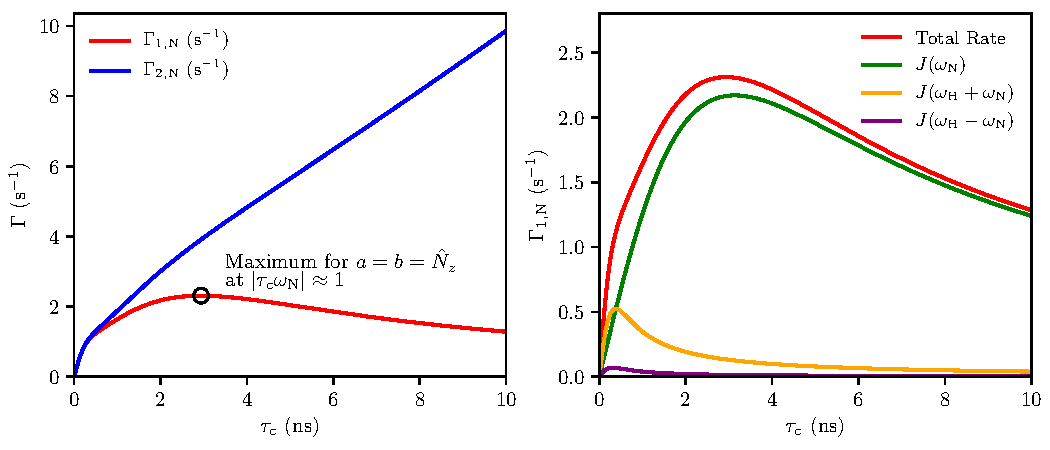
\includegraphics[scale=0.85]{./Figures/SimonsFigs/AppendixBFig.pdf}
\caption{i. Plots of longitudinal ($a = b = \hat{N}_z$) and transverse ($a = b = \hat{N}^+$) nitrogen relaxation rates for an ensemble of $^{15}$N-$^{1}$H spin pairs, whose only relaxation mechanism is the dipolar interaction, undergoing spherical isotropic motion, as a function of $\tau_{\text{c}}$. Parameters used: $B_0 = 11.74 \si{\tesla}$ (corresponding to a $500 \si{\mega \hertz}$ magnet), $\gamma_{\text{H}} = \num{2.675e8} \si{\tesla\per\second}$, $\gamma_{\text{N}} = \num{-2.712e7} \si{\tesla\per\second}$, $r_{\text{NH}} = \num{1.02} \si{\angstrom}$. ii. Plots of the individual contributions to the transverse nitrogen relaxation rate, as a function of $\tau_{\text{c}}$.}
\label{figB.1}
\end{figure}

To gain an appreciation of how the to relaxation rates calculated in sections \ref{secB.2} and \ref{secB.3} vary with rotational correlation time, a $^{15}$N-$^{1}$H dipolar system is considered, in a magnetic field of $\num{11.74} \si{\tesla}$, corresponding to a $\num{500} \si{\mega \hertz}$ magnet. Figure \ref{figB.1} illustrates the nitrogen longitudinal and transverse relaxation rates for such a system. \\
For transverse relaxation, beyond $\tau_{\text{c}} \approx 2 \si{\nano\second}$, there is a linear dependence of rate with $\tau_{\text{c}}$. This is since the $J(0)$ term present in \ref{eqB.7} is dominant for large $\tau_{\text{c}}$ values, and the transverse relaxation rate can conveniently be collapsed to:
\begin{equation}
\Gamma_{2,\text{N}} \approx \frac{d_{\text{IS}}^2 \tau_{\text{c}}}{5}  
\end{equation}
For longitudinal relaxation, no such linear dependence is seen, as there isn't a contribution from $J(0)$. The dominant term in $\Gamma_{1,\text{N}}$, for large $\tau_{\text{c}}$ values is $J(\omega_{\text{N}})$, as this is the term with the smallest associated frequency magnitude. Therefore, a maximum occurs very close to the $\tau_{\text{c}}$ value where $J(\omega_{\text{N}})$ reaches a maximum, i.e. $|\omega_{\text{N}} \tau_{\text{c}}| \approx 1$. The three individual contributions to the expression of $\Gamma_{1,\text{N}}$, expressed in \ref{eqB.5}, are plotted in figure \ref{figB.1}. For each of these contributions, a maximum appears when $|\omega \tau_{c}| = 1$, which yields a spectral density of $\frac{\tau_{\text{c}}}{2}$.
\section{Noteworthy Identities}
The following section provides a list of a number of the identities used in the calculations above
\subsection{Operator Products}
\begin{equation*}
\begin{gathered}
\hat{I}_z \hat{I}^- = -\frac{1}{2} \hat{I}^- \hspace{20pt} \hat{I}^- \hat{I}_z = \frac{1}{2} \hat{I}^- \hspace{20pt} \hat{I}_z \hat{I}^+ = \frac{1}{2} \hat{I}^+ \hspace{20pt} \hat{I}^+ \hat{I}_z = -\frac{1}{2} \hat{I}^+ \\
\hat{I}^+ \hat{I}^- = \frac{1}{2} \hat{E} + \hat{I}_z \hspace{3pt} (= \hat{I}^{\alpha}) \hspace{20pt} \hat{I}^- \hat{I}^+ = \frac{1}{2} \hat{E} - \hat{I}_z \hspace{3pt} (= \hat{I}^{\beta})
\end{gathered}
\end{equation*}
\subsection{Commutators}
\begin{equation*}
\begin{gathered}
\comm{\hat{I}_z}{\hat{I}^+} = \hat{I}_z \hat{I}^+ - \hat{I}^+ \hat{I}_z = \hat{I}^+ \hspace{20pt}
\comm{\hat{I}_z}{\hat{I}^-} = \hat{I}_z \hat{I}^- - \hat{I}^- \hat{I}_z = -\hat{I}^- \\
\comm{\hat{I}^+}{\hat{I}^-} = \hat{I}^+ \hat{I}^- - \hat{I}^- \hat{I}^+ = \hat{I}^{\alpha} - \hat{I}^{\beta} = 2 \hat{I}_z \\
\comm{\hat{I}^+ \hat{S}^+}{\hat{I}^- \hat{S}^-} = \hat{I}^+ \hat{I}^- \hat{S}^+ \hat{S}^- - \hat{I}^- \hat{I}^+ \hat{S}^- \hat{S}^+ = \hat{I}_z + \hat{S}_z \\
\comm{\hat{I}^+ \hat{S}^-}{\hat{I}^- \hat{S}^+} = \hat{I}^+ \hat{I}^- \hat{S}^- \hat{S}^+ - \hat{I}^- \hat{I}^+ \hat{S}^+ \hat{S}^- = \hat{I}_z - \hat{S}_z
\end{gathered}
\end{equation*}
\subsection{Expectation Values}
\begin{align*}
&\bra{\hat{I}_z} \ket{\hat{I}_z} = \expval{\hat{I}_z^2} = \frac{1}{4} \expval{\hat{E}} = \frac{1}{4} \left[\bra{\alpha \alpha} \ket{\alpha \alpha} + \bra{\alpha \beta} \ket{\alpha \beta} + \bra{\beta \alpha} \ket{\beta \alpha} + \bra{\beta \beta} \ket{\beta \beta}\right] \\
&\hspace{41pt}= 1 \\
&\bra{\hat{I}_z} \ket{\hat{I}_z + \hat{S}_z} = \expval{\hat{I}_z^2 + \hat{I}_z \hat{S}_z} = \expval{\frac{1}{4} \hat{E} + \hat{I}_z \hat{S}_z} \\
&\hspace{67pt}= \bigg[\mel{\alpha \alpha}{\frac{1}{4} \hat{E} + \hat{I}_z\hat{S}_z}{\alpha \alpha} + \mel{\alpha \beta}{\frac{1}{4} \hat{E} + \hat{I}_z\hat{S}_z}{\alpha \beta} \\
&\hspace{88pt} + \mel{\beta \alpha}{\frac{1}{4} \hat{E} + \hat{I}_z\hat{S}_z}{\beta \alpha} + \mel{\beta \beta}{\frac{1}{4} \hat{E} + \hat{I}_z\hat{S}_z}{\beta \beta} \bigg] \\
&\hspace{67pt} = \frac{1}{2} \left[\bra{\alpha \alpha} \ket{\alpha \alpha} + \bra{\beta \beta} \ket{\beta \beta}\right] \\
& \hspace{67pt} = 1 \\
&\bra{\hat{I}_z} \ket{\hat{I}^- \hat{S}^+} = -\frac{1}{2}\expval{\hat{I}^- \hat{S}^+} \\
& \hspace{59pt} = -\frac{1}{2} \big[ \mel{\alpha \alpha}{\hat{I}^- \hat{S}^+}{\alpha\alpha} + \mel{\alpha \beta}{\hat{I}^- \hat{S}^+}{\alpha\beta}  \\
& \hspace{95pt} + \mel{\beta \alpha}{\hat{I}^- \hat{S}^+}{\beta\alpha} + \mel{\beta \beta}{\hat{I}^- \hat{S}^+}{\beta\beta} \big] \\
& \hspace{59pt} = -\frac{1}{2} \bra{\beta \alpha} \ket{\alpha \beta} \\
& \hspace{59pt} = 0 \\
&\bra{\hat{I}^+} \ket{\hat{I}^+} = \expval{\hat{I}^- \hat{I}^+} = \expval{\frac{1}{2} \hat{E} - \hat{I}_z} \\
& \hspace{48pt}= \bigg[\mel{\alpha \alpha}{\frac{1}{2} \hat{E} - \hat{I}_z}{\alpha \alpha} + \mel{\alpha \beta}{\frac{1}{2} \hat{E} - \hat{I}_z}{\alpha \beta} \\
&\hspace{69pt} + \mel{\beta \alpha}{\frac{1}{2} \hat{E} - \hat{I}_z}{\beta \alpha} + \mel{\beta \beta}{\frac{1}{2} \hat{E} - \hat{I}_z}{\beta \beta} \bigg] \\
& \hspace{48pt}= \bra{\alpha \alpha} \ket{\alpha \alpha} + \bra{\alpha \beta} \ket{\alpha \beta} \\
& \hspace{48pt} = 2
\end{align*}

\begin{singlespacing}
\printappendixbibliography
\end{singlespacing}
\end{appendixtext}

% !TeX root = ./Report-Body.tex
\chapter{I$_3$S Rate Expressions}
\allowdisplaybreaks

\begin{appendixtext}
In this appendix, full expressions of the relaxation rates, $\Gamma_{2,\text{S}}^i$, where\\$i \in \{\alpha \alpha \alpha, \alpha \alpha\beta, \alpha\beta\beta, \beta\beta\beta\}$, for each model considered in Figure \ref{CH3Models}, are presented. Definitions of the dipolar and chemical shift interaction constants are given in \ref{DipConst} and \ref{CSAConst}. If not defined below, the spectral density functions of relevance are given in \ref{SpecDenSpher} and \ref{SpecDenMeth}. $P_i^{(2)} (x)$ denotes the associated Legendre polynomial of degree 2 and order i, where $i \in \{0, 1, 2\}$. These have a close link to the 2$^{\text{nd}}$ rank reduced Wigner-d matrix elements, and are commonly used in their place in the literature:
\begin{equation}
\begin{split}
&P_0^{(2)}(\cos \beta) = \frac{1}{2}\left( 3 \cos^2 \beta -1 \right) = d_{0,0}^{2} (\beta) \\
&P_1^{(2)}(\cos \beta) = -3\cos \beta \sin \beta = - \sqrt{6} d_{0,1}^{(2)}(\beta) = \sqrt{6} d_{0,-1}^{(2)}(\beta) \\
&P_2^{(2)}(\cos \beta) = 3\sin^2 \beta = \sqrt{6} d_{0,2}^{(2)}(\beta) = \sqrt{6} d_{0,-2}^{(2)}(\beta)
\end{split}
\end{equation}\\
 $\beta$ is the angle between the methyl threefold rotation axis, and the $^{13}$C-$^1$H bond vectors (set to be $\ang{109.47}$ in all calculations conducted in this thesis).
\section{Diffusive/Woessner Models (Plots i. and ii.)}
\footnotesize
\begin{equation*}
\begin{split}
\Gamma_{2,S}^{\alpha\alpha\alpha}&=d_{\text{IS}}^2P_2^{(2)}(\cos\beta)^2\bigg[\frac{1}{80}J\left(\frac{\tau_{\text{c}}\tau_{\text{m}}}{\tau_{\text{m}}+k_{\text{DW}}^2\tau_{\text{c}}},\omega_{\text{I}}-\omega_{\text{S}}\right)+\frac{3}{80}J\left(\frac{\tau_{\text{c}}\tau_{\text{m}}}{\tau_{\text{m}}+k_{\text{DW}}^2\tau_{\text{c}}},\omega_{\text{I}}\right) \\ 
&\hspace{90pt}+\frac{3}{40}J\left(\frac{\tau_{\text{c}}\tau_{\text{m}}}{\tau_{\text{m}}+k_{\text{DW}}^2\tau_{\text{c}}},\omega_{\text{I}}+\omega_{\text{S}}\right)\bigg] \\
&\hspace{4pt}+d_{\text{IS}}^2P_1^{(2)}(\cos\beta)^2\bigg[\frac{9}{320}J\left(\frac{\tau_{\text{c}}\tau_{\text{m}}}{\tau_{\text{m}}+\tau_{\text{c}}},\omega_{\text{I}}-\omega_{\text{S}}\right)+\frac{27}{320}J\left(\frac{\tau_{\text{c}}\tau_{\text{m}}}{\tau_{\text{m}}+\tau_{\text{c}}},\omega_{\text{I}}\right) \\ 
&\hspace{90pt}+\frac{27}{160}J\left(\frac{\tau_{\text{c}}\tau_{\text{m}}}{\tau_{\text{m}}+\tau_{\text{c}}},\omega_{\text{I}}+\omega_{\text{S}}\right)\bigg] \\
&\hspace{4pt}+d_{\text{IS}}^2P_0^{(2)}(\cos\beta)^2\bigg[\frac{9}{5}J(\tau_{\text{c}},0)+\frac{3}{20}J\left(\tau_{\text{c}},\omega_{\text{I}}-\omega_{\text{S}}\right)+\frac{27}{20}J\left(\tau_{\text{c}},\omega_{\text{S}}\right)+\frac{9}{20}J\left(\tau_{\text{c}},\omega_{\text{I}}\right) \\ 
&\hspace{90pt}+\frac{9}{10}J\left(\tau_{\text{c}},\omega_{\text{I}}+\omega_{\text{S}}\right)\bigg] \\
&\hspace{4pt}+d_{\text{IS}}c_{\text{S}}P_0^{(2)}(\cos\beta)\bigg[-\frac{4}{5}J\left(\tau_{\text{c}},0\right)-\frac{3}{5}J\left(\tau_{\text{c}},\omega_{\text{S}}\right)\bigg] \\
&\hspace{4pt}+d_{\text{II}}^2\bigg[\frac{27}{80}J\left(\frac{\tau_{\text{c}}\tau_{\text{m}}}{\tau_{\text{m}}+k_{\text{DW}}^2\tau_{\text{c}}},\omega_{\text{I}}\right)+\frac{9}{20}J\left(\tau_{\text{c}},\omega_{\text{I}}\right)+\frac{27}{20}J\left(\frac{\tau_{\text{c}}\tau_{\text{m}}}{\tau_{\text{m}}+k_{\text{DW}}^2\tau_{\text{c}}},2\omega_{\text{I}}\right)+\frac{9}{20}J\left(\tau_{\text{c}},2\omega_{\text{I}}\right)\bigg] \\
&\hspace{4pt}- \frac{3}{20} d_{\text{II}}c_{\text{I}}P_2^{(2)}(\cos\beta) J\left(\frac{\tau_{\text{c}}\tau_{\text{m}}}{\tau_{\text{m}}+k_{\text{DW}}^2\tau_{\text{c}}},\omega_{\text{I}}\right)+ \frac{3}{5} d_{\text{II}}c_{\text{I}}P_0^{(2)}(\cos\beta) J\left(\tau_{\text{c}},\omega_{\text{I}}\right) \\ 
&\hspace{4pt}+\frac{1}{60} c_{\text{I}}^2P_2^{(2)}(\cos\beta)^2 J\left(\frac{\tau_{\text{c}}\tau_{\text{m}}}{\tau_{\text{m}}+k_{\text{DW}}^2\tau_{\text{c}}},\omega_{\text{I}}\right)+\frac{3}{80} c_{\text{I}}^2P_1^{(2)}(\cos\beta)^2 J\left(\frac{\tau_{\text{c}}\tau_{\text{m}}}{\tau_{\text{m}}+\tau_{\text{c}}},\omega_{\text{I}}\right) \\
&\hspace{4pt}+\frac{1}{5} c_{\text{I}}^2P_0^{(2)}(\cos\beta)^2J\left(\tau_{\text{c}},\omega_{\text{I}}\right)+c_{\text{S}}^2\bigg[\frac{4}{45}J\left(\tau_{\text{c}},0\right)+\frac{1}{15}J(\tau_{\text{c}},\omega_{\text{S}})\bigg] \\
&\hspace{4pt} +\Gamma_{\text{ext}}
\end{split}
\end{equation*}
\begin{equation*}
\begin{split}
\Gamma_{2,S}^{\alpha\alpha\beta}&=d_{\text{IS}}^2P_2^{(2)}(\cos\beta)^2\bigg[\frac{3}{45}J\left(\frac{\tau_{\text{c}}\tau_{\text{m}}}{\tau_{\text{m}}+k_{\text{DW}}^2\tau_{\text{c}}},0\right) + \frac{1}{20}J\left(\frac{\tau_{\text{c}}\tau_{\text{m}}}{\tau_{\text{m}}+k_{\text{DW}}^2\tau_{\text{c}}},\omega_{\text{S}}\right) \\
&\hspace{90pt}+ \frac{1}{80}J\left(\frac{\tau_{\text{c}}\tau_{\text{m}}}{\tau_{\text{m}}+k_{\text{DW}}^2\tau_{\text{c}}},\omega_{\text{I}}-\omega_{\text{S}}\right)+\frac{3}{80}J\left(\frac{\tau_{\text{c}}\tau_{\text{m}}}{\tau_{\text{m}}+k_{\text{DW}}^2\tau_{\text{c}}},\omega_{\text{I}}\right) \\
&\hspace{90pt}+\frac{3}{40}J\left(\frac{\tau_{\text{c}}\tau_{\text{m}}}{\tau_{\text{m}}+k_{\text{DW}}^2\tau_{\text{c}}},\omega_{\text{I}}+\omega_{\text{S}}\right)\bigg] \\
&\hspace{4pt}+d_{\text{IS}}^2P_1^{(2)}(\cos\beta)^2\bigg[\frac{3}{20}J\left(\frac{\tau_{\text{c}}\tau_{\text{m}}}{\tau_{\text{m}}+\tau_{\text{c}}},0\right)+ \frac{9}{80}J\left(\frac{\tau_{\text{c}}\tau_{\text{m}}}{\tau_{\text{m}}+k_{\text{DW}}^2\tau_{\text{c}}},\omega_{\text{S}}\right) + \frac{9}{320}J\left(\frac{\tau_{\text{c}}\tau_{\text{m}}}{\tau_{\text{m}}+\tau_{\text{c}}},\omega_{\text{I}}-\omega_{\text{S}}\right)\\
&\hspace{90pt} +\frac{27}{320}J\left(\frac{\tau_{\text{c}}\tau_{\text{m}}}{\tau_{\text{m}}+\tau_{\text{c}}},\omega_{\text{I}}\right) +\frac{27}{160}J\left(\frac{\tau_{\text{c}}\tau_{\text{m}}}{\tau_{\text{m}}+\tau_{\text{c}}},\omega_{\text{I}}+\omega_{\text{S}}\right)\bigg] \\
&\hspace{4pt}+d_{\text{IS}}^2P_0^{(2)}(\cos\beta)^2\bigg[\frac{1}{5}J(\tau_{\text{c}},0)+\frac{3}{20}J\left(\tau_{\text{c}},\omega_{\text{I}}-\omega_{\text{S}}\right)+\frac{3}{20}J\left(\tau_{\text{c}},\omega_{\text{S}}\right)+\frac{9}{20}J\left(\tau_{\text{c}},\omega_{\text{I}}\right) \\ 
&\hspace{90pt}+\frac{9}{10}J\left(\tau_{\text{c}},\omega_{\text{I}}+\omega_{\text{S}}\right)\bigg] \\
&\hspace{4pt}+d_{\text{IS}}c_{\text{S}}P_0^{(2)}(\cos\beta)\bigg[-\frac{4}{15}J\left(\tau_{\text{c}},0\right)-\frac{1}{5}J\left(\tau_{\text{c}},\omega_{\text{S}}\right)\bigg] \\
&\hspace{4pt}+d_{\text{II}}^2\bigg[\frac{63}{80}J\left(\frac{\tau_{\text{c}}\tau_{\text{m}}}{\tau_{\text{m}}+k_{\text{DW}}^2\tau_{\text{c}}},\omega_{\text{I}}\right)+\frac{3}{20}J\left(\tau_{\text{c}},\omega_{\text{I}}\right)+\frac{9}{20}J\left(\frac{\tau_{\text{c}}\tau_{\text{m}}}{\tau_{\text{m}}+k_{\text{DW}}^2\tau_{\text{c}}},2\omega_{\text{I}}\right)+\frac{3}{20}J\left(\tau_{\text{c}},2\omega_{\text{I}}\right)\bigg] \\
&\hspace{4pt}- \frac{1}{20} d_{\text{II}}c_{\text{I}}P_2^{(2)}(\cos\beta) J\left(\frac{\tau_{\text{c}}\tau_{\text{m}}}{\tau_{\text{m}}+k_{\text{DW}}^2\tau_{\text{c}}},\omega_{\text{I}}\right)+ \frac{1}{5} d_{\text{II}}c_{\text{I}}P_0^{(2)}(\cos\beta) J\left(\tau_{\text{c}},\omega_{\text{I}}\right) \\ 
&\hspace{4pt}+\frac{1}{60} c_{\text{I}}^2P_2^{(2)}(\cos\beta)^2 J\left(\frac{\tau_{\text{c}}\tau_{\text{m}}}{\tau_{\text{m}}+k_{\text{DW}}^2\tau_{\text{c}}},\omega_{\text{I}}\right)+\frac{3}{80} c_{\text{I}}^2P_1^{(2)}(\cos\beta)^2 J\left(\frac{\tau_{\text{c}}\tau_{\text{m}}}{\tau_{\text{m}}+\tau_{\text{c}}},\omega_{\text{I}}\right) \\
&\hspace{4pt}+\frac{1}{5} c_{\text{I}}^2P_0^{(2)}(\cos\beta)^2J\left(\tau_{\text{c}},\omega_{\text{I}}\right)+c_{\text{S}}^2\bigg[\frac{4}{45}J\left(\tau_{\text{c}},0\right)+\frac{1}{15}J(\tau_{\text{c}},\omega_{\text{S}})\bigg]\\
&\hspace{4pt} +\Gamma_{\text{ext}}
\end{split}
\end{equation*}
\begin{equation*}
\begin{split}
\Gamma_{2,S}^{\alpha\beta\beta}&=d_{\text{IS}}^2P_2^{(2)}(\cos\beta)^2\bigg[\frac{3}{45}J\left(\frac{\tau_{\text{c}}\tau_{\text{m}}}{\tau_{\text{m}}+k_{\text{DW}}^2\tau_{\text{c}}},0\right) + \frac{1}{20}J\left(\frac{\tau_{\text{c}}\tau_{\text{m}}}{\tau_{\text{m}}+k_{\text{DW}}^2\tau_{\text{c}}},\omega_{\text{S}}\right) \\
&\hspace{90pt}+ \frac{1}{80}J\left(\frac{\tau_{\text{c}}\tau_{\text{m}}}{\tau_{\text{m}}+k_{\text{DW}}^2\tau_{\text{c}}},\omega_{\text{I}}-\omega_{\text{S}}\right)+\frac{3}{80}J\left(\frac{\tau_{\text{c}}\tau_{\text{m}}}{\tau_{\text{m}}+k_{\text{DW}}^2\tau_{\text{c}}},\omega_{\text{I}}\right) \\
&\hspace{90pt}+\frac{3}{40}J\left(\frac{\tau_{\text{c}}\tau_{\text{m}}}{\tau_{\text{m}}+k_{\text{DW}}^2\tau_{\text{c}}},\omega_{\text{I}}+\omega_{\text{S}}\right)\bigg] \\
&\hspace{4pt}+d_{\text{IS}}^2P_1^{(2)}(\cos\beta)^2\bigg[\frac{3}{20}J\left(\frac{\tau_{\text{c}}\tau_{\text{m}}}{\tau_{\text{m}}+\tau_{\text{c}}},0\right)+ \frac{9}{80}J\left(\frac{\tau_{\text{c}}\tau_{\text{m}}}{\tau_{\text{m}}+k_{\text{DW}}^2\tau_{\text{c}}},\omega_{\text{S}}\right) + \frac{9}{320}J\left(\frac{\tau_{\text{c}}\tau_{\text{m}}}{\tau_{\text{m}}+\tau_{\text{c}}},\omega_{\text{I}}-\omega_{\text{S}}\right)\\
&\hspace{90pt} +\frac{27}{320}J\left(\frac{\tau_{\text{c}}\tau_{\text{m}}}{\tau_{\text{m}}+\tau_{\text{c}}},\omega_{\text{I}}\right) +\frac{27}{160}J\left(\frac{\tau_{\text{c}}\tau_{\text{m}}}{\tau_{\text{m}}+\tau_{\text{c}}},\omega_{\text{I}}+\omega_{\text{S}}\right)\bigg] \\
&\hspace{4pt}+d_{\text{IS}}^2P_0^{(2)}(\cos\beta)^2\bigg[\frac{1}{5}J(\tau_{\text{c}},0)+\frac{3}{20}J\left(\tau_{\text{c}},\omega_{\text{I}}-\omega_{\text{S}}\right)+\frac{3}{20}J\left(\tau_{\text{c}},\omega_{\text{S}}\right)+\frac{9}{20}J\left(\tau_{\text{c}},\omega_{\text{I}}\right) \\ 
&\hspace{90pt}+\frac{9}{10}J\left(\tau_{\text{c}},\omega_{\text{I}}+\omega_{\text{S}}\right)\bigg] \\
&\hspace{4pt}+d_{\text{IS}}c_{\text{S}}P_0^{(2)}(\cos\beta)\bigg[\frac{4}{15}J\left(\tau_{\text{c}},0\right)+\frac{1}{5}J\left(\tau_{\text{c}},\omega_{\text{S}}\right)\bigg] \\
&\hspace{4pt}+d_{\text{II}}^2\bigg[\frac{63}{80}J\left(\frac{\tau_{\text{c}}\tau_{\text{m}}}{\tau_{\text{m}}+k_{\text{DW}}^2\tau_{\text{c}}},\omega_{\text{I}}\right)+\frac{3}{20}J\left(\tau_{\text{c}},\omega_{\text{I}}\right)+\frac{9}{20}J\left(\frac{\tau_{\text{c}}\tau_{\text{m}}}{\tau_{\text{m}}+k_{\text{DW}}^2\tau_{\text{c}}},2\omega_{\text{I}}\right)+\frac{3}{20}J\left(\tau_{\text{c}},2\omega_{\text{I}}\right)\bigg] \\
&\hspace{4pt}+ \frac{1}{20} d_{\text{II}}c_{\text{I}}P_2^{(2)}(\cos\beta) J\left(\frac{\tau_{\text{c}}\tau_{\text{m}}}{\tau_{\text{m}}+k_{\text{DW}}^2\tau_{\text{c}}},\omega_{\text{I}}\right)- \frac{1}{5} d_{\text{II}}c_{\text{I}}P_0^{(2)}(\cos\beta) J\left(\tau_{\text{c}},\omega_{\text{I}}\right) \\ 
&\hspace{4pt}+\frac{1}{60} c_{\text{I}}^2P_2^{(2)}(\cos\beta)^2 J\left(\frac{\tau_{\text{c}}\tau_{\text{m}}}{\tau_{\text{m}}+k_{\text{DW}}^2\tau_{\text{c}}},\omega_{\text{I}}\right)+\frac{3}{80} c_{\text{I}}^2P_1^{(2)}(\cos\beta)^2 J\left(\frac{\tau_{\text{c}}\tau_{\text{m}}}{\tau_{\text{m}}+\tau_{\text{c}}},\omega_{\text{I}}\right) \\
&\hspace{4pt}+\frac{1}{5} c_{\text{I}}^2P_0^{(2)}(\cos\beta)^2J\left(\tau_{\text{c}},\omega_{\text{I}}\right)+c_{\text{S}}^2\bigg[\frac{4}{45}J\left(\tau_{\text{c}},0\right)+\frac{1}{15}J(\tau_{\text{c}},\omega_{\text{S}})\bigg]\\
&\hspace{4pt} +\Gamma_{\text{ext}}
\end{split}
\end{equation*}
\begin{equation*}
\begin{split}
\Gamma_{2,S}^{\beta\beta\beta}&=d_{\text{IS}}^2P_2^{(2)}(\cos\beta)^2\bigg[\frac{1}{80}J\left(\frac{\tau_{\text{c}}\tau_{\text{m}}}{\tau_{\text{m}}+k_{\text{DW}}^2\tau_{\text{c}}},\omega_{\text{I}}-\omega_{\text{S}}\right)+\frac{3}{80}J\left(\frac{\tau_{\text{c}}\tau_{\text{m}}}{\tau_{\text{m}}+k_{\text{DW}}^2\tau_{\text{c}}},\omega_{\text{I}}\right) \\ 
&\hspace{90pt}+\frac{3}{40}J\left(\frac{\tau_{\text{c}}\tau_{\text{m}}}{\tau_{\text{m}}+k_{\text{DW}}^2\tau_{\text{c}}},\omega_{\text{I}}+\omega_{\text{S}}\right)\bigg] \\
&\hspace{4pt}+d_{\text{IS}}^2P_1^{(2)}(\cos\beta)^2\bigg[\frac{9}{320}J\left(\frac{\tau_{\text{c}}\tau_{\text{m}}}{\tau_{\text{m}}+\tau_{\text{c}}},\omega_{\text{I}}-\omega_{\text{S}}\right)+\frac{27}{320}J\left(\frac{\tau_{\text{c}}\tau_{\text{m}}}{\tau_{\text{m}}+\tau_{\text{c}}},\omega_{\text{I}}\right) \\ 
&\hspace{90pt}+\frac{27}{160}J\left(\frac{\tau_{\text{c}}\tau_{\text{m}}}{\tau_{\text{m}}+\tau_{\text{c}}},\omega_{\text{I}}+\omega_{\text{S}}\right)\bigg] \\
&\hspace{4pt}+d_{\text{IS}}^2P_0^{(2)}(\cos\beta)^2\bigg[\frac{9}{5}J(\tau_{\text{c}},0)+\frac{3}{20}J\left(\tau_{\text{c}},\omega_{\text{I}}-\omega_{\text{S}}\right)+\frac{27}{20}J\left(\tau_{\text{c}},\omega_{\text{S}}\right)+\frac{9}{20}J\left(\tau_{\text{c}},\omega_{\text{I}}\right) \\ 
&\hspace{90pt}+\frac{9}{10}J\left(\tau_{\text{c}},\omega_{\text{I}}+\omega_{\text{S}}\right)\bigg] \\
&\hspace{4pt}+d_{\text{IS}}c_{\text{S}}P_0^{(2)}(\cos\beta)\bigg[\frac{4}{5}J\left(\tau_{\text{c}},0\right)+\frac{3}{5}J\left(\tau_{\text{c}},\omega_{\text{S}}\right)\bigg] \\
&\hspace{4pt}+d_{\text{II}}^2\bigg[\frac{27}{80}J\left(\frac{\tau_{\text{c}}\tau_{\text{m}}}{\tau_{\text{m}}+k_{\text{DW}}^2\tau_{\text{c}}},\omega_{\text{I}}\right)+\frac{9}{20}J\left(\tau_{\text{c}},\omega_{\text{I}}\right)+\frac{27}{20}J\left(\frac{\tau_{\text{c}}\tau_{\text{m}}}{\tau_{\text{m}}+k_{\text{DW}}^2\tau_{\text{c}}},2\omega_{\text{I}}\right)+\frac{9}{20}J\left(\tau_{\text{c}},2\omega_{\text{I}}\right)\bigg] \\
&\hspace{4pt}+ \frac{3}{20} d_{\text{II}}c_{\text{I}}P_2^{(2)}(\cos\beta) J\left(\frac{\tau_{\text{c}}\tau_{\text{m}}}{\tau_{\text{m}}+k_{\text{DW}}^2\tau_{\text{c}}},\omega_{\text{I}}\right)- \frac{3}{5} d_{\text{II}}c_{\text{I}}P_0^{(2)}(\cos\beta) J\left(\tau_{\text{c}},\omega_{\text{I}}\right) \\ 
&\hspace{4pt}+\frac{1}{60} c_{\text{I}}^2P_2^{(2)}(\cos\beta)^2 J\left(\frac{\tau_{\text{c}}\tau_{\text{m}}}{\tau_{\text{m}}+k_{\text{DW}}^2\tau_{\text{c}}},\omega_{\text{I}}\right)+\frac{3}{80} c_{\text{I}}^2P_1^{(2)}(\cos\beta)^2 J\left(\frac{\tau_{\text{c}}\tau_{\text{m}}}{\tau_{\text{m}}+\tau_{\text{c}}},\omega_{\text{I}}\right) \\
&\hspace{4pt}+\frac{1}{5} c_{\text{I}}^2P_0^{(2)}(\cos\beta)^2J\left(\tau_{\text{c}},\omega_{\text{I}}\right)+c_{\text{S}}^2\bigg[\frac{4}{45}J\left(\tau_{\text{c}},0\right)+\frac{1}{15}J(\tau_{\text{c}},\omega_{\text{S}})\bigg] \\
&\hspace{4pt} +\Gamma_{\text{ext}}
\end{split}
\end{equation*}
where $k_{\text{DW}} = 1$ for the Woessner model, and $k_{\text{DW}} = 2$ for the diffusive model. $\Gamma_{\text{ext}}$ is given in \ref{External}. \\
\section{Spherical Isotropic Motion (Plot iii.)}
\begin{equation*}
\begin{split}
\Gamma_{2,S}^{\alpha\alpha\alpha}&=d_{\text{IS}}^2P_2^{(2)}(\cos\beta)^2\bigg[\frac{1}{80}J\left(\tau_{\text{c}},\omega_{\text{I}}-\omega_{\text{S}}\right)+\frac{3}{80}J\left(\tau_{\text{c}},\omega_{\text{I}}\right) +\frac{3}{40}J\left(\tau_{\text{c}},\omega_{\text{I}}+\omega_{\text{S}}\right)\bigg] \\
&\hspace{4pt}+d_{\text{IS}}^2P_1^{(2)}(\cos\beta)^2\bigg[\frac{9}{320}J\left(\tau_{\text{c}},\omega_{\text{I}}-\omega_{\text{S}}\right)+\frac{27}{320}J\left(\tau_{\text{c}},\omega_{\text{I}}\right)+\frac{27}{160}J\left(\tau_{\text{c}},\omega_{\text{I}}+\omega_{\text{S}}\right)\bigg] \\
&\hspace{4pt}+d_{\text{IS}}^2P_0^{(2)}(\cos\beta)^2\bigg[\frac{9}{5}J(\tau_{\text{c}},0)+\frac{3}{20}J\left(\tau_{\text{c}},\omega_{\text{I}}-\omega_{\text{S}}\right)+\frac{27}{20}J\left(\tau_{\text{c}},\omega_{\text{S}}\right)+\frac{9}{20}J\left(\tau_{\text{c}},\omega_{\text{I}}\right) \\ 
&\hspace{90pt}+\frac{9}{10}J\left(\tau_{\text{c}},\omega_{\text{I}}+\omega_{\text{S}}\right)\bigg] \\
&\hspace{4pt}+d_{\text{IS}}c_{\text{S}}P_0^{(2)}(\cos\beta)\bigg[-\frac{4}{5}J\left(\tau_{\text{c}},0\right)-\frac{3}{5}J\left(\tau_{\text{c}},\omega_{\text{S}}\right)\bigg] \\
&\hspace{4pt}+d_{\text{II}}^2\bigg[\frac{63}{80}J\left(\tau_{\text{c}},\omega_{\text{I}}\right)+ \frac{9}{5}J\left(\tau_{\text{c}},2\omega_{\text{I}}\right)\bigg] \\
&\hspace{4pt}- \frac{9}{20} d_{\text{II}}c_{\text{I}}P_2^{(2)}(\cos\beta) J\left(\tau_{\text{c}},\omega_{\text{I}}\right)+ \frac{3}{5} d_{\text{II}}c_{\text{I}}P_0^{(2)}(\cos\beta) J\left(\tau_{\text{c}},\omega_{\text{I}}\right) \\ 
&\hspace{4pt}+\frac{1}{60} c_{\text{I}}^2P_2^{(2)}(\cos\beta)^2 J\left(\tau_{\text{c}},\omega_{\text{I}}\right)+\frac{3}{80} c_{\text{I}}^2P_1^{(2)}(\cos\beta)^2 J\left(\tau_{\text{c}},\omega_{\text{I}}\right) \\
&\hspace{4pt}+\frac{1}{5} c_{\text{I}}^2P_0^{(2)}(\cos\beta)^2J\left(\tau_{\text{c}},\omega_{\text{I}}\right)+c_{\text{S}}^2\bigg[\frac{4}{45}J\left(\tau_{\text{c}},0\right)+\frac{1}{15}J(\tau_{\text{c}},\omega_{\text{S}})\bigg] \\
&\hspace{4pt} +\Gamma_{\text{ext}}
\end{split}
\end{equation*}
\begin{equation*}
\begin{split}
\Gamma_{2,S}^{\alpha\alpha\beta}&=d_{\text{IS}}^2P_2^{(2)}(\cos\beta)^2\bigg[\frac{3}{45}J\left(\tau_{\text{c}},0\right) + \frac{1}{20}J\left(\tau_{\text{c}},\omega_{\text{S}}\right)
+ \frac{1}{80}J\left(\tau_{\text{c}},\omega_{\text{I}}-\omega_{\text{S}}\right)\\
&\hspace{90pt}+\frac{3}{80}J\left(\tau_{\text{c}},\omega_{\text{I}}\right)+\frac{3}{40}J\left(\tau_{\text{c}},\omega_{\text{I}}+\omega_{\text{S}}\right)\bigg] \\
&\hspace{4pt}+d_{\text{IS}}^2P_1^{(2)}(\cos\beta)^2\bigg[\frac{3}{20}J\left(\tau_{\text{c}},0\right)+ \frac{9}{80}J\left(\tau_{\text{c}},\omega_{\text{S}}\right) + \frac{9}{320}J\left(\tau_{\text{c}},\omega_{\text{I}}-\omega_{\text{S}}\right)\\
&\hspace{90pt} +\frac{27}{320}J\left(\tau_{\text{c}},\omega_{\text{I}}\right) +\frac{27}{160}J\left(\tau_{\text{c}},\omega_{\text{I}}+\omega_{\text{S}}\right)\bigg] \\
&\hspace{4pt}+d_{\text{IS}}^2P_0^{(2)}(\cos\beta)^2\bigg[\frac{1}{5}J(\tau_{\text{c}},0)+\frac{3}{20}J\left(\tau_{\text{c}},\omega_{\text{I}}-\omega_{\text{S}}\right)+\frac{3}{20}J\left(\tau_{\text{c}},\omega_{\text{S}}\right)+\frac{9}{20}J\left(\tau_{\text{c}},\omega_{\text{I}}\right) \\ 
&\hspace{90pt}+\frac{9}{10}J\left(\tau_{\text{c}},\omega_{\text{I}}+\omega_{\text{S}}\right)\bigg] \\
&\hspace{4pt}+d_{\text{IS}}c_{\text{S}}P_0^{(2)}(\cos\beta)\bigg[-\frac{4}{15}J\left(\tau_{\text{c}},0\right)-\frac{1}{5}J\left(\tau_{\text{c}},\omega_{\text{S}}\right)\bigg] \\
&\hspace{4pt}+d_{\text{II}}^2\bigg[+\frac{15}{16}J\left(\tau_{\text{c}},\omega_{\text{I}}\right)+\frac{3}{5}J\left(\tau_{\text{c}},2\omega_{\text{I}}\right)\bigg] \\
&\hspace{4pt}- \frac{1}{20} d_{\text{II}}c_{\text{I}}P_2^{(2)}(\cos\beta) J\left(\tau_{\text{c}},\omega_{\text{I}}\right)+ \frac{1}{5} d_{\text{II}}c_{\text{I}}P_0^{(2)}(\cos\beta) J\left(\tau_{\text{c}},\omega_{\text{I}}\right) \\ 
&\hspace{4pt}+\frac{1}{60} c_{\text{I}}^2P_2^{(2)}(\cos\beta)^2 J\left(\tau_{\text{c}},\omega_{\text{I}}\right)+\frac{3}{80} c_{\text{I}}^2P_1^{(2)}(\cos\beta)^2 J\left(\tau_{\text{c}},\omega_{\text{I}}\right) \\
&\hspace{4pt}+\frac{1}{5} c_{\text{I}}^2P_0^{(2)}(\cos\beta)^2J\left(\tau_{\text{c}},\omega_{\text{I}}\right)+c_{\text{S}}^2\bigg[\frac{4}{45}J\left(\tau_{\text{c}},0\right)+\frac{1}{15}J(\tau_{\text{c}},\omega_{\text{S}})\bigg]\\
&\hspace{4pt} +\Gamma_{\text{ext}}
\end{split}
\end{equation*}
\begin{equation*}
\begin{split}
\Gamma_{2,S}^{\alpha\beta\beta}&=d_{\text{IS}}^2P_2^{(2)}(\cos\beta)^2\bigg[\frac{3}{45}J\left(\tau_{\text{c}},0\right) + \frac{1}{20}J\left(\tau_{\text{c}},\omega_{\text{S}}\right)
+ \frac{1}{80}J\left(\tau_{\text{c}},\omega_{\text{I}}-\omega_{\text{S}}\right)\\
&\hspace{90pt}+\frac{3}{80}J\left(\tau_{\text{c}},\omega_{\text{I}}\right)+\frac{3}{40}J\left(\tau_{\text{c}},\omega_{\text{I}}+\omega_{\text{S}}\right)\bigg] \\
&\hspace{4pt}+d_{\text{IS}}^2P_1^{(2)}(\cos\beta)^2\bigg[\frac{3}{20}J\left(\tau_{\text{c}},0\right)+ \frac{9}{80}J\left(\tau_{\text{c}},\omega_{\text{S}}\right) + \frac{9}{320}J\left(\tau_{\text{c}},\omega_{\text{I}}-\omega_{\text{S}}\right)\\
&\hspace{90pt} +\frac{27}{320}J\left(\tau_{\text{c}},\omega_{\text{I}}\right) +\frac{27}{160}J\left(\tau_{\text{c}},\omega_{\text{I}}+\omega_{\text{S}}\right)\bigg] \\
&\hspace{4pt}+d_{\text{IS}}^2P_0^{(2)}(\cos\beta)^2\bigg[\frac{1}{5}J(\tau_{\text{c}},0)+\frac{3}{20}J\left(\tau_{\text{c}},\omega_{\text{I}}-\omega_{\text{S}}\right)+\frac{3}{20}J\left(\tau_{\text{c}},\omega_{\text{S}}\right)+\frac{9}{20}J\left(\tau_{\text{c}},\omega_{\text{I}}\right) \\ 
&\hspace{90pt}+\frac{9}{10}J\left(\tau_{\text{c}},\omega_{\text{I}}+\omega_{\text{S}}\right)\bigg] \\
&\hspace{4pt}+d_{\text{IS}}c_{\text{S}}P_0^{(2)}(\cos\beta)\bigg[\frac{4}{15}J\left(\tau_{\text{c}},0\right)+\frac{1}{5}J\left(\tau_{\text{c}},\omega_{\text{S}}\right)\bigg] \\
&\hspace{4pt}+d_{\text{II}}^2\bigg[+\frac{15}{16}J\left(\tau_{\text{c}},\omega_{\text{I}}\right)+\frac{3}{5}J\left(\tau_{\text{c}},2\omega_{\text{I}}\right)\bigg] \\
&\hspace{4pt}+ \frac{1}{20} d_{\text{II}}c_{\text{I}}P_2^{(2)}(\cos\beta) J\left(\tau_{\text{c}},\omega_{\text{I}}\right)- \frac{1}{5} d_{\text{II}}c_{\text{I}}P_0^{(2)}(\cos\beta) J\left(\tau_{\text{c}},\omega_{\text{I}}\right) \\ 
&\hspace{4pt}+\frac{1}{60} c_{\text{I}}^2P_2^{(2)}(\cos\beta)^2 J\left(\tau_{\text{c}},\omega_{\text{I}}\right)+\frac{3}{80} c_{\text{I}}^2P_1^{(2)}(\cos\beta)^2 J\left(\tau_{\text{c}},\omega_{\text{I}}\right) \\
&\hspace{4pt}+\frac{1}{5} c_{\text{I}}^2P_0^{(2)}(\cos\beta)^2J\left(\tau_{\text{c}},\omega_{\text{I}}\right)+c_{\text{S}}^2\bigg[\frac{4}{45}J\left(\tau_{\text{c}},0\right)+\frac{1}{15}J(\tau_{\text{c}},\omega_{\text{S}})\bigg]\\
&\hspace{4pt} +\Gamma_{\text{ext}}
\end{split}
\end{equation*}
\begin{equation*}
\begin{split}
\Gamma_{2,S}^{\beta\beta\beta}&=d_{\text{IS}}^2P_2^{(2)}(\cos\beta)^2\bigg[\frac{1}{80}J\left(\tau_{\text{c}},\omega_{\text{I}}-\omega_{\text{S}}\right)+\frac{3}{80}J\left(\tau_{\text{c}},\omega_{\text{I}}\right) +\frac{3}{40}J\left(\tau_{\text{c}},\omega_{\text{I}}+\omega_{\text{S}}\right)\bigg] \\
&\hspace{4pt}+d_{\text{IS}}^2P_1^{(2)}(\cos\beta)^2\bigg[\frac{9}{320}J\left(\tau_{\text{c}},\omega_{\text{I}}-\omega_{\text{S}}\right)+\frac{27}{320}J\left(\tau_{\text{c}},\omega_{\text{I}}\right)+\frac{27}{160}J\left(\tau_{\text{c}},\omega_{\text{I}}+\omega_{\text{S}}\right)\bigg] \\
&\hspace{4pt}+d_{\text{IS}}^2P_0^{(2)}(\cos\beta)^2\bigg[\frac{9}{5}J(\tau_{\text{c}},0)+\frac{3}{20}J\left(\tau_{\text{c}},\omega_{\text{I}}-\omega_{\text{S}}\right)+\frac{27}{20}J\left(\tau_{\text{c}},\omega_{\text{S}}\right)+\frac{9}{20}J\left(\tau_{\text{c}},\omega_{\text{I}}\right) \\ 
&\hspace{90pt}+\frac{9}{10}J\left(\tau_{\text{c}},\omega_{\text{I}}+\omega_{\text{S}}\right)\bigg] \\
&\hspace{4pt}+d_{\text{IS}}c_{\text{S}}P_0^{(2)}(\cos\beta)\bigg[\frac{4}{5}J\left(\tau_{\text{c}},0\right)+\frac{3}{5}J\left(\tau_{\text{c}},\omega_{\text{S}}\right)\bigg] \\
&\hspace{4pt}+d_{\text{II}}^2\bigg[\frac{63}{80}J\left(\tau_{\text{c}},\omega_{\text{I}}\right)+ \frac{9}{5}J\left(\tau_{\text{c}},2\omega_{\text{I}}\right)\bigg] \\
&\hspace{4pt}+ \frac{9}{20} d_{\text{II}}c_{\text{I}}P_2^{(2)}(\cos\beta) J\left(\tau_{\text{c}},\omega_{\text{I}}\right)- \frac{3}{5} d_{\text{II}}c_{\text{I}}P_0^{(2)}(\cos\beta) J\left(\tau_{\text{c}},\omega_{\text{I}}\right) \\ 
&\hspace{4pt}+\frac{1}{60} c_{\text{I}}^2P_2^{(2)}(\cos\beta)^2 J\left(\tau_{\text{c}},\omega_{\text{I}}\right)+\frac{3}{80} c_{\text{I}}^2P_1^{(2)}(\cos\beta)^2 J\left(\tau_{\text{c}},\omega_{\text{I}}\right) \\
&\hspace{4pt}+\frac{1}{5} c_{\text{I}}^2P_0^{(2)}(\cos\beta)^2J\left(\tau_{\text{c}},\omega_{\text{I}}\right)+c_{\text{S}}^2\bigg[\frac{4}{45}J\left(\tau_{\text{c}},0\right)+\frac{1}{15}J(\tau_{\text{c}},\omega_{\text{S}})\bigg] \\
&\hspace{4pt} +\Gamma_{\text{ext}}
\end{split}
\end{equation*}
\section{Ollerenshaw et al. (Plot iv.)}
\begin{equation*}
\Gamma_{2,S}^{\alpha\alpha\alpha} = \Gamma_{2,S}^{\beta\beta\beta} = \frac{1}{5} d_{\text{IS}}^2 S_{\text{axis}}^2 \tau_{\text{c}} + \Gamma_{\text{ext}}
\end{equation*}
\begin{equation*}
\Gamma_{2,S}^{\alpha\alpha\beta} = \Gamma_{2,S}^{\alpha\beta\beta} = \frac{1}{45} d_{\text{IS}}^2 S_{\text{axis}}^2 \tau_{\text{c}} + \Gamma_{\text{ext}}
\end{equation*}
where $\Gamma_{\text{ext}} = \frac{3\tau_{\text{c}}}{20}\sum\limits_i d_{\text{II},i}$
\section{Hansen et al. (Plot v.)}
\begin{equation*}
\begin{split}
&\Gamma_{2,S}^{\alpha\alpha\alpha} = \frac{1}{20}\left(\frac{2}{3}c_{\text{S}}-3d_{\text{IS}}P_0^{(2)}(\cos\beta)\right)^2\left(4J(0)+3J(\omega_{\text{S}})\right) \\
&\hspace{41pt}+ \left(\frac{1}{2}d_{\text{IS}}^2P_1^{(2)}(\cos\beta)^2+\frac{1}{8}d_{\text{IS}}^2P_2^{(2)}(\cos\beta)^2+\frac{27}{16}d_{\text{II}}^2\right)\tau_{\text{m}}
\end{split}
\end{equation*}
\begin{equation*}
\begin{split}
&\Gamma_{2,S}^{\alpha\alpha\beta} = \frac{1}{20}\left(\frac{2}{3}c_{\text{S}}-d_{\text{IS}}P_0^{(2)}(\cos\beta)\right)^2\left(4J(0)+3J(\omega_{\text{S}})\right) \\
&\hspace{41pt}+ \left(\frac{29}{30}d_{\text{IS}}^2P_1^{(2)}(\cos\beta)^2+\frac{29}{120}d_{\text{IS}}^2P_2^{(2)}(\cos\beta)^2+\frac{99}{80}d_{\text{II}}^2\right)\tau_{\text{m}}
\end{split}
\end{equation*}
\begin{equation*}
\begin{split}
&\Gamma_{2,S}^{\alpha\beta\beta} = \frac{1}{20}\left(\frac{2}{3}c_{\text{S}}+d_{\text{IS}}P_0^{(2)}(\cos\beta)\right)^2\left(4J(0)+3J(\omega_{\text{S}})\right) \\
&\hspace{41pt}+ \left(\frac{29}{30}d_{\text{IS}}^2P_1^{(2)}(\cos\beta)^2+\frac{29}{120}d_{\text{IS}}^2P_2^{(2)}(\cos\beta)^2+\frac{99}{80}d_{\text{II}}^2\right)\tau_{\text{m}}
\end{split}
\end{equation*}
\begin{equation*}
\begin{split}
&\Gamma_{2,S}^{\beta\beta\beta} = \frac{1}{20}\left(\frac{2}{3}c_{\text{S}}+3d_{\text{IS}}P_0^{(2)}(\cos\beta)\right)^2\left(4J(0)+3J(\omega_{\text{S}})\right) \\
&\hspace{41pt}+ \left(\frac{1}{2}d_{\text{IS}}^2P_1^{(2)}(\cos\beta)^2+\frac{1}{8}d_{\text{IS}}^2P_2^{(2)}(\cos\beta)^2+\frac{27}{16}d_{\text{II}}^2\right)\tau_{\text{m}}
\end{split}
\end{equation*}
where the spectral density function, $J(\omega)$ is defined by:
\begin{equation*}
\begin{split}
&J(\omega)=S_{\text{axis}}^2\frac{\tau_{\text{c}}}{1+\omega^2\tau_{\text{c}}^2}+(1-S_{\text{axis}}^2)\frac{\tau_1}{1+\omega^2\tau_1^2}, \\
&\frac{1}{\tau_1}=\frac{1}{\tau_{\text{c}}}+\frac{1}{\tau_{\text{axis}}}
\end{split}
\end{equation*}
\begin{singlespacing}
\printappendixbibliography
\end{singlespacing}
\end{appendixtext}



%\include{Report-AppendixPaper}% Uncomment this line and see
%                              % the instructions in
%                              % Report-AppendixPaper.tex if
%                              % you wish to append a paper.
%%%%%
% Include the spine only when you are doing the final
% printing of your thesis
% % !TeX root = ./Report-Body.tex
\setlength{\textheight}{260mm}
\setlength{\textwidth}{140mm}

\setlength{\voffset}{-23mm} 
\setlength{\hoffset}{-10mm}



\thispagestyle{empty}

\begin{landscape}

\begin{large} \textbf{\theauthor} \hfill \textbf{\thetitle} \hfill \textbf{\thecollege} \end{large}
 
\vspace*{\stretch{0.3}}

\begin{large} \textbf{\theauthor} \hfill \textbf{\thetitle} \hfill \textbf{\thecollege} \end{large}


\vspace*{\stretch{0.3}}

\begin{large} \textbf{\theauthor} \hfill \textbf{\thetitle} \hfill \textbf{\thecollege} \end{large}

\vspace*{\stretch{0.3}}

\begin{large} \textbf{\theauthor} \hfill \textbf{\thetitle} \hfill \textbf{\thecollege} \end{large}


\end{landscape}
\pagebreak


\end{document}
